\documentclass[twoside]{book}

% Packages required by doxygen
\usepackage{fixltx2e}
\usepackage{calc}
\usepackage{doxygen}
\usepackage[export]{adjustbox} % also loads graphicx
\usepackage{graphicx}
\usepackage[utf8]{inputenc}
\usepackage{makeidx}
\usepackage{multicol}
\usepackage{multirow}
\PassOptionsToPackage{warn}{textcomp}
\usepackage{textcomp}
\usepackage[nointegrals]{wasysym}
\usepackage[table]{xcolor}

% Font selection
\usepackage[T1]{fontenc}
\usepackage[scaled=.90]{helvet}
\usepackage{courier}
\usepackage{amssymb}
\usepackage{sectsty}
\renewcommand{\familydefault}{\sfdefault}
\allsectionsfont{%
  \fontseries{bc}\selectfont%
  \color{darkgray}%
}
\renewcommand{\DoxyLabelFont}{%
  \fontseries{bc}\selectfont%
  \color{darkgray}%
}
\newcommand{\+}{\discretionary{\mbox{\scriptsize$\hookleftarrow$}}{}{}}

% Page & text layout
\usepackage{geometry}
\geometry{%
  a4paper,%
  top=2.5cm,%
  bottom=2.5cm,%
  left=2.5cm,%
  right=2.5cm%
}
\tolerance=750
\hfuzz=15pt
\hbadness=750
\setlength{\emergencystretch}{15pt}
\setlength{\parindent}{0cm}
\setlength{\parskip}{3ex plus 2ex minus 2ex}
\makeatletter
\renewcommand{\paragraph}{%
  \@startsection{paragraph}{4}{0ex}{-1.0ex}{1.0ex}{%
    \normalfont\normalsize\bfseries\SS@parafont%
  }%
}
\renewcommand{\subparagraph}{%
  \@startsection{subparagraph}{5}{0ex}{-1.0ex}{1.0ex}{%
    \normalfont\normalsize\bfseries\SS@subparafont%
  }%
}
\makeatother

% Headers & footers
\usepackage{fancyhdr}
\pagestyle{fancyplain}
\fancyhead[LE]{\fancyplain{}{\bfseries\thepage}}
\fancyhead[CE]{\fancyplain{}{}}
\fancyhead[RE]{\fancyplain{}{\bfseries\leftmark}}
\fancyhead[LO]{\fancyplain{}{\bfseries\rightmark}}
\fancyhead[CO]{\fancyplain{}{}}
\fancyhead[RO]{\fancyplain{}{\bfseries\thepage}}
\fancyfoot[LE]{\fancyplain{}{}}
\fancyfoot[CE]{\fancyplain{}{}}
\fancyfoot[RE]{\fancyplain{}{\bfseries\scriptsize Generated by Doxygen }}
\fancyfoot[LO]{\fancyplain{}{\bfseries\scriptsize Generated by Doxygen }}
\fancyfoot[CO]{\fancyplain{}{}}
\fancyfoot[RO]{\fancyplain{}{}}
\renewcommand{\footrulewidth}{0.4pt}
\renewcommand{\chaptermark}[1]{%
  \markboth{#1}{}%
}
\renewcommand{\sectionmark}[1]{%
  \markright{\thesection\ #1}%
}

% Indices & bibliography
\usepackage{natbib}
\usepackage[titles]{tocloft}
\setcounter{tocdepth}{3}
\setcounter{secnumdepth}{5}
\makeindex

% Hyperlinks (required, but should be loaded last)
\usepackage{ifpdf}
\ifpdf
  \usepackage[pdftex,pagebackref=true]{hyperref}
\else
  \usepackage[ps2pdf,pagebackref=true]{hyperref}
\fi
\hypersetup{%
  colorlinks=true,%
  linkcolor=blue,%
  citecolor=blue,%
  unicode%
}

% Custom commands
\newcommand{\clearemptydoublepage}{%
  \newpage{\pagestyle{empty}\cleardoublepage}%
}

\usepackage{caption}
\captionsetup{labelsep=space,justification=centering,font={bf},singlelinecheck=off,skip=4pt,position=top}

%===== C O N T E N T S =====

\begin{document}

% Titlepage & ToC
\hypersetup{pageanchor=false,
             bookmarksnumbered=true,
             pdfencoding=unicode
            }
\pagenumbering{alph}
\begin{titlepage}
\vspace*{7cm}
\begin{center}%
{\Large My Project }\\
\vspace*{1cm}
{\large Generated by Doxygen 1.8.13}\\
\end{center}
\end{titlepage}
\clearemptydoublepage
\pagenumbering{roman}
\tableofcontents
\clearemptydoublepage
\pagenumbering{arabic}
\hypersetup{pageanchor=true}

%--- Begin generated contents ---
\chapter{Namespace Index}
\section{Namespace List}
Here is a list of all namespaces with brief descriptions\+:\begin{DoxyCompactList}
\item\contentsline{section}{\hyperlink{namespaceUi}{Ui} }{\pageref{namespaceUi}}{}
\end{DoxyCompactList}

\chapter{Hierarchical Index}
\section{Class Hierarchy}
This inheritance list is sorted roughly, but not completely, alphabetically\+:\begin{DoxyCompactList}
\item \contentsline{section}{Calcul\+Comparaison}{\pageref{classCalculComparaison}}{}
\item \contentsline{section}{Heuristique}{\pageref{classHeuristique}}{}
\item \contentsline{section}{Instance}{\pageref{classInstance}}{}
\item \contentsline{section}{Methode\+Exacte}{\pageref{classMethodeExacte}}{}
\item Q\+Dialog\begin{DoxyCompactList}
\item \contentsline{section}{Comparaison\+Solution}{\pageref{classComparaisonSolution}}{}
\item \contentsline{section}{Generation\+Instance}{\pageref{classGenerationInstance}}{}
\item \contentsline{section}{Resolution\+Instance}{\pageref{classResolutionInstance}}{}
\end{DoxyCompactList}
\item Q\+Main\+Window\begin{DoxyCompactList}
\item \contentsline{section}{Fenetre\+Principale}{\pageref{classFenetrePrincipale}}{}
\end{DoxyCompactList}
\item Q\+Object\begin{DoxyCompactList}
\item \contentsline{section}{Worker\+Comparaison}{\pageref{classWorkerComparaison}}{}
\item \contentsline{section}{Worker\+Dossier}{\pageref{classWorkerDossier}}{}
\item \contentsline{section}{Worker\+Fichier}{\pageref{classWorkerFichier}}{}
\item \contentsline{section}{Worker\+Instance}{\pageref{classWorkerInstance}}{}
\end{DoxyCompactList}
\item \contentsline{section}{Resultat}{\pageref{classResultat}}{}
\end{DoxyCompactList}

\chapter{Class Index}
\section{Class List}
Here are the classes, structs, unions and interfaces with brief descriptions\+:\begin{DoxyCompactList}
\item\contentsline{section}{\hyperlink{classComparaisonSolution}{Comparaison\+Solution} }{\pageref{classComparaisonSolution}}{}
\item\contentsline{section}{\hyperlink{classCreationInstance}{Creation\+Instance} }{\pageref{classCreationInstance}}{}
\item\contentsline{section}{\hyperlink{classFenetrePrincipale}{Fenetre\+Principale} \\*La Fenêtre Principale }{\pageref{classFenetrePrincipale}}{}
\item\contentsline{section}{\hyperlink{classGenerationInstance}{Generation\+Instance} \\*La fenêtre de génération d\textquotesingle{}instance }{\pageref{classGenerationInstance}}{}
\item\contentsline{section}{\hyperlink{classHeuristique}{Heuristique} \\*Classe \hyperlink{classHeuristique}{Heuristique} permetant de trier et affecter des jobs sur des machines }{\pageref{classHeuristique}}{}
\item\contentsline{section}{\hyperlink{classInstance}{Instance} \\*Classe représentant une instance }{\pageref{classInstance}}{}
\item\contentsline{section}{\hyperlink{classMethodeExacte}{Methode\+Exacte} \\*Classe \hyperlink{classMethodeExacte}{Methode\+Exacte} permetant de résoudre des instances à l\textquotesingle{}aide de méthodes exactes }{\pageref{classMethodeExacte}}{}
\item\contentsline{section}{\hyperlink{classResolutionInstance}{Resolution\+Instance} \\*Fenêtre \hyperlink{classResolutionInstance}{Resolution\+Instance} }{\pageref{classResolutionInstance}}{}
\item\contentsline{section}{\hyperlink{classWorkerComparaison}{Worker\+Comparaison} \\*Le Worker permetant de gérer la comparaison d\textquotesingle{}un dossier de résultats }{\pageref{classWorkerComparaison}}{}
\item\contentsline{section}{\hyperlink{classWorkerDossier}{Worker\+Dossier} \\*Le Worker permetant de gérer la résolution d\textquotesingle{}un dossier d\textquotesingle{}instances }{\pageref{classWorkerDossier}}{}
\item\contentsline{section}{\hyperlink{classWorkerFichier}{Worker\+Fichier} \\*Le Worker permetant de gérer la résolution d\textquotesingle{}un fichier d\textquotesingle{}instance }{\pageref{classWorkerFichier}}{}
\item\contentsline{section}{\hyperlink{classWorkerInstance}{Worker\+Instance} \\*Le Worker permetant de gérer la génération de fichiers d\textquotesingle{}instance }{\pageref{classWorkerInstance}}{}
\end{DoxyCompactList}

\chapter{File Index}
\section{File List}
Here is a list of all files with brief descriptions\+:\begin{DoxyCompactList}
\item\contentsline{section}{P\+R\+D\+Ordonancement/\hyperlink{comparaisonsolution_8cpp}{comparaisonsolution.\+cpp} }{\pageref{comparaisonsolution_8cpp}}{}
\item\contentsline{section}{P\+R\+D\+Ordonancement/\hyperlink{comparaisonsolution_8h}{comparaisonsolution.\+h} }{\pageref{comparaisonsolution_8h}}{}
\item\contentsline{section}{P\+R\+D\+Ordonancement/\hyperlink{fenetreprincipale_8cpp}{fenetreprincipale.\+cpp} }{\pageref{fenetreprincipale_8cpp}}{}
\item\contentsline{section}{P\+R\+D\+Ordonancement/\hyperlink{fenetreprincipale_8h}{fenetreprincipale.\+h} }{\pageref{fenetreprincipale_8h}}{}
\item\contentsline{section}{P\+R\+D\+Ordonancement/\hyperlink{generationinstance_8cpp}{generationinstance.\+cpp} }{\pageref{generationinstance_8cpp}}{}
\item\contentsline{section}{P\+R\+D\+Ordonancement/\hyperlink{generationinstance_8h}{generationinstance.\+h} }{\pageref{generationinstance_8h}}{}
\item\contentsline{section}{P\+R\+D\+Ordonancement/\hyperlink{heuristique_8cpp}{heuristique.\+cpp} }{\pageref{heuristique_8cpp}}{}
\item\contentsline{section}{P\+R\+D\+Ordonancement/\hyperlink{heuristique_8h}{heuristique.\+h} }{\pageref{heuristique_8h}}{}
\item\contentsline{section}{P\+R\+D\+Ordonancement/\hyperlink{instance_8cpp}{instance.\+cpp} }{\pageref{instance_8cpp}}{}
\item\contentsline{section}{P\+R\+D\+Ordonancement/\hyperlink{instance_8h}{instance.\+h} }{\pageref{instance_8h}}{}
\item\contentsline{section}{P\+R\+D\+Ordonancement/\hyperlink{main_8cpp}{main.\+cpp} }{\pageref{main_8cpp}}{}
\item\contentsline{section}{P\+R\+D\+Ordonancement/\hyperlink{methodeexacte_01_07copy_011_08_8cpp}{methodeexacte (copy 1).\+cpp} }{\pageref{methodeexacte_01_07copy_011_08_8cpp}}{}
\item\contentsline{section}{P\+R\+D\+Ordonancement/\hyperlink{methodeexacte_8cpp}{methodeexacte.\+cpp} }{\pageref{methodeexacte_8cpp}}{}
\item\contentsline{section}{P\+R\+D\+Ordonancement/\hyperlink{methodeexacte_8h}{methodeexacte.\+h} }{\pageref{methodeexacte_8h}}{}
\item\contentsline{section}{P\+R\+D\+Ordonancement/\hyperlink{plne_8cpp}{plne.\+cpp} }{\pageref{plne_8cpp}}{}
\item\contentsline{section}{P\+R\+D\+Ordonancement/\hyperlink{plne_8h}{plne.\+h} }{\pageref{plne_8h}}{}
\item\contentsline{section}{P\+R\+D\+Ordonancement/\hyperlink{plnemip2_8cpp}{plnemip2.\+cpp} }{\pageref{plnemip2_8cpp}}{}
\item\contentsline{section}{P\+R\+D\+Ordonancement/\hyperlink{plnemip2_8h}{plnemip2.\+h} }{\pageref{plnemip2_8h}}{}
\item\contentsline{section}{P\+R\+D\+Ordonancement/\hyperlink{resolutioninstance_8cpp}{resolutioninstance.\+cpp} }{\pageref{resolutioninstance_8cpp}}{}
\item\contentsline{section}{P\+R\+D\+Ordonancement/\hyperlink{resolutioninstance_8h}{resolutioninstance.\+h} }{\pageref{resolutioninstance_8h}}{}
\item\contentsline{section}{P\+R\+D\+Ordonancement/\hyperlink{workercomparaison_8cpp}{workercomparaison.\+cpp} }{\pageref{workercomparaison_8cpp}}{}
\item\contentsline{section}{P\+R\+D\+Ordonancement/\hyperlink{workercomparaison_8h}{workercomparaison.\+h} }{\pageref{workercomparaison_8h}}{}
\item\contentsline{section}{P\+R\+D\+Ordonancement/\hyperlink{workerdossier_8cpp}{workerdossier.\+cpp} }{\pageref{workerdossier_8cpp}}{}
\item\contentsline{section}{P\+R\+D\+Ordonancement/\hyperlink{workerdossier_8h}{workerdossier.\+h} }{\pageref{workerdossier_8h}}{}
\item\contentsline{section}{P\+R\+D\+Ordonancement/\hyperlink{workerfichier_8cpp}{workerfichier.\+cpp} }{\pageref{workerfichier_8cpp}}{}
\item\contentsline{section}{P\+R\+D\+Ordonancement/\hyperlink{workerfichier_8h}{workerfichier.\+h} }{\pageref{workerfichier_8h}}{}
\item\contentsline{section}{P\+R\+D\+Ordonancement/\hyperlink{workerinstance_8cpp}{workerinstance.\+cpp} }{\pageref{workerinstance_8cpp}}{}
\item\contentsline{section}{P\+R\+D\+Ordonancement/\hyperlink{workerinstance_8h}{workerinstance.\+h} }{\pageref{workerinstance_8h}}{}
\end{DoxyCompactList}

\chapter{Namespace Documentation}
\hypertarget{namespaceUi}{}\section{Ui Namespace Reference}
\label{namespaceUi}\index{Ui@{Ui}}

\chapter{Class Documentation}
\hypertarget{classComparaisonSolution}{}\section{Comparaison\+Solution Class Reference}
\label{classComparaisonSolution}\index{Comparaison\+Solution@{Comparaison\+Solution}}


{\ttfamily \#include $<$comparaisonsolution.\+h$>$}



Inheritance diagram for Comparaison\+Solution\+:
\nopagebreak
\begin{figure}[H]
\begin{center}
\leavevmode
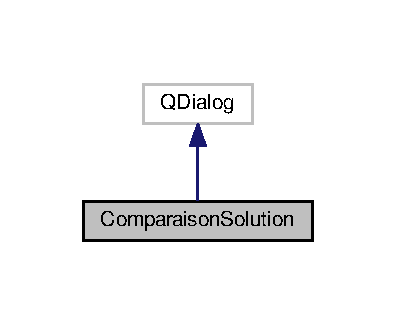
\includegraphics[width=190pt]{classComparaisonSolution__inherit__graph}
\end{center}
\end{figure}


Collaboration diagram for Comparaison\+Solution\+:
\nopagebreak
\begin{figure}[H]
\begin{center}
\leavevmode
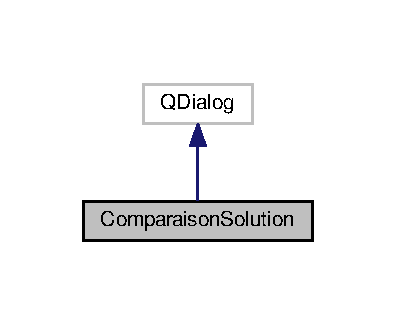
\includegraphics[width=190pt]{classComparaisonSolution__coll__graph}
\end{center}
\end{figure}
\subsection*{Public Member Functions}
\begin{DoxyCompactItemize}
\item 
\hyperlink{classComparaisonSolution_a7fc9723f5a627d53e331719c3f47c7cc}{Comparaison\+Solution} (Q\+Widget $\ast$parent=0)
\item 
\hyperlink{classComparaisonSolution_a07a910b473173981273789934cf34e7f}{$\sim$\+Comparaison\+Solution} ()
\end{DoxyCompactItemize}


\subsection{Constructor \& Destructor Documentation}
\mbox{\Hypertarget{classComparaisonSolution_a7fc9723f5a627d53e331719c3f47c7cc}\label{classComparaisonSolution_a7fc9723f5a627d53e331719c3f47c7cc}} 
\index{Comparaison\+Solution@{Comparaison\+Solution}!Comparaison\+Solution@{Comparaison\+Solution}}
\index{Comparaison\+Solution@{Comparaison\+Solution}!Comparaison\+Solution@{Comparaison\+Solution}}
\subsubsection{\texorpdfstring{Comparaison\+Solution()}{ComparaisonSolution()}}
{\footnotesize\ttfamily Comparaison\+Solution\+::\+Comparaison\+Solution (\begin{DoxyParamCaption}\item[{Q\+Widget $\ast$}]{parent = {\ttfamily 0} }\end{DoxyParamCaption})\hspace{0.3cm}{\ttfamily [explicit]}}

\mbox{\Hypertarget{classComparaisonSolution_a07a910b473173981273789934cf34e7f}\label{classComparaisonSolution_a07a910b473173981273789934cf34e7f}} 
\index{Comparaison\+Solution@{Comparaison\+Solution}!````~Comparaison\+Solution@{$\sim$\+Comparaison\+Solution}}
\index{````~Comparaison\+Solution@{$\sim$\+Comparaison\+Solution}!Comparaison\+Solution@{Comparaison\+Solution}}
\subsubsection{\texorpdfstring{$\sim$\+Comparaison\+Solution()}{~ComparaisonSolution()}}
{\footnotesize\ttfamily Comparaison\+Solution\+::$\sim$\+Comparaison\+Solution (\begin{DoxyParamCaption}{ }\end{DoxyParamCaption})}



The documentation for this class was generated from the following files\+:\begin{DoxyCompactItemize}
\item 
P\+R\+D\+Ordonancement/\hyperlink{comparaisonsolution_8h}{comparaisonsolution.\+h}\item 
P\+R\+D\+Ordonancement/\hyperlink{comparaisonsolution_8cpp}{comparaisonsolution.\+cpp}\end{DoxyCompactItemize}

\hypertarget{classCreationInstance}{}\section{Creation\+Instance Class Reference}
\label{classCreationInstance}\index{Creation\+Instance@{Creation\+Instance}}


{\ttfamily \#include $<$creationinstance.\+h$>$}

\subsection*{Public Member Functions}
\begin{DoxyCompactItemize}
\item 
\hyperlink{classCreationInstance_af3d5a102616539b753a82ea83cded735}{Creation\+Instance} ()
\end{DoxyCompactItemize}


\subsection{Constructor \& Destructor Documentation}
\mbox{\Hypertarget{classCreationInstance_af3d5a102616539b753a82ea83cded735}\label{classCreationInstance_af3d5a102616539b753a82ea83cded735}} 
\index{Creation\+Instance@{Creation\+Instance}!Creation\+Instance@{Creation\+Instance}}
\index{Creation\+Instance@{Creation\+Instance}!Creation\+Instance@{Creation\+Instance}}
\subsubsection{\texorpdfstring{Creation\+Instance()}{CreationInstance()}}
{\footnotesize\ttfamily Creation\+Instance\+::\+Creation\+Instance (\begin{DoxyParamCaption}{ }\end{DoxyParamCaption})}



The documentation for this class was generated from the following files\+:\begin{DoxyCompactItemize}
\item 
P\+R\+D\+Ordonancement/\hyperlink{creationinstance_8h}{creationinstance.\+h}\item 
P\+R\+D\+Ordonancement/\hyperlink{creationinstance_8cpp}{creationinstance.\+cpp}\end{DoxyCompactItemize}

\hypertarget{classFenetrePrincipale}{}\section{Fenetre\+Principale Class Reference}
\label{classFenetrePrincipale}\index{Fenetre\+Principale@{Fenetre\+Principale}}


La Fenêtre Principale.  




{\ttfamily \#include $<$fenetreprincipale.\+h$>$}



Inheritance diagram for Fenetre\+Principale\+:\nopagebreak
\begin{figure}[H]
\begin{center}
\leavevmode
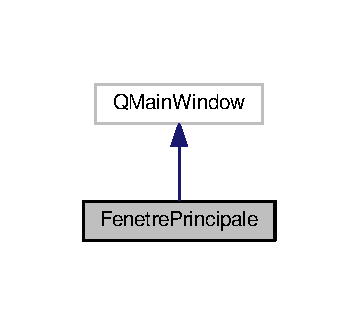
\includegraphics[width=172pt]{classFenetrePrincipale__inherit__graph}
\end{center}
\end{figure}


Collaboration diagram for Fenetre\+Principale\+:\nopagebreak
\begin{figure}[H]
\begin{center}
\leavevmode
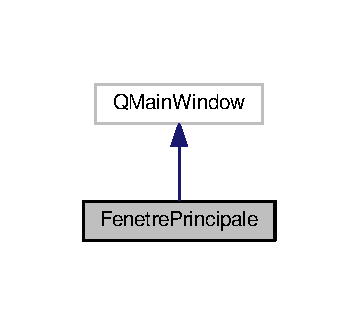
\includegraphics[width=172pt]{classFenetrePrincipale__coll__graph}
\end{center}
\end{figure}
\subsection*{Public Member Functions}
\begin{DoxyCompactItemize}
\item 
\hyperlink{classFenetrePrincipale_aab8cf15535ca6934db27e5e45e2b6d7b}{Fenetre\+Principale} (Q\+Widget $\ast$parent=0)
\begin{DoxyCompactList}\small\item\em Constructeur de la Fenêtre Principale. \end{DoxyCompactList}\item 
\hyperlink{classFenetrePrincipale_afb035ceb7a4f1ddd23ab6213b582efa1}{$\sim$\+Fenetre\+Principale} ()
\begin{DoxyCompactList}\small\item\em Destructeur de la Fenêtre Principale. \end{DoxyCompactList}\end{DoxyCompactItemize}


\subsection{Detailed Description}
La Fenêtre Principale. 

\subsection{Constructor \& Destructor Documentation}
\mbox{\Hypertarget{classFenetrePrincipale_aab8cf15535ca6934db27e5e45e2b6d7b}\label{classFenetrePrincipale_aab8cf15535ca6934db27e5e45e2b6d7b}} 
\index{Fenetre\+Principale@{Fenetre\+Principale}!Fenetre\+Principale@{Fenetre\+Principale}}
\index{Fenetre\+Principale@{Fenetre\+Principale}!Fenetre\+Principale@{Fenetre\+Principale}}
\subsubsection{\texorpdfstring{Fenetre\+Principale()}{FenetrePrincipale()}}
{\footnotesize\ttfamily Fenetre\+Principale\+::\+Fenetre\+Principale (\begin{DoxyParamCaption}\item[{Q\+Widget $\ast$}]{parent = {\ttfamily 0} }\end{DoxyParamCaption})\hspace{0.3cm}{\ttfamily [explicit]}}



Constructeur de la Fenêtre Principale. 


\begin{DoxyParams}{Parameters}
{\em parent} & \\
\hline
\end{DoxyParams}
\mbox{\Hypertarget{classFenetrePrincipale_afb035ceb7a4f1ddd23ab6213b582efa1}\label{classFenetrePrincipale_afb035ceb7a4f1ddd23ab6213b582efa1}} 
\index{Fenetre\+Principale@{Fenetre\+Principale}!````~Fenetre\+Principale@{$\sim$\+Fenetre\+Principale}}
\index{````~Fenetre\+Principale@{$\sim$\+Fenetre\+Principale}!Fenetre\+Principale@{Fenetre\+Principale}}
\subsubsection{\texorpdfstring{$\sim$\+Fenetre\+Principale()}{~FenetrePrincipale()}}
{\footnotesize\ttfamily Fenetre\+Principale\+::$\sim$\+Fenetre\+Principale (\begin{DoxyParamCaption}{ }\end{DoxyParamCaption})}



Destructeur de la Fenêtre Principale. 



The documentation for this class was generated from the following files\+:\begin{DoxyCompactItemize}
\item 
P\+R\+D\+Ordonancement/\hyperlink{fenetreprincipale_8h}{fenetreprincipale.\+h}\item 
P\+R\+D\+Ordonancement/\hyperlink{fenetreprincipale_8cpp}{fenetreprincipale.\+cpp}\end{DoxyCompactItemize}

\hypertarget{classGenerationInstance}{}\section{Generation\+Instance Class Reference}
\label{classGenerationInstance}\index{Generation\+Instance@{Generation\+Instance}}


La fenêtre de génération d\textquotesingle{}instance.  




{\ttfamily \#include $<$generationinstance.\+h$>$}



Inheritance diagram for Generation\+Instance\+:\nopagebreak
\begin{figure}[H]
\begin{center}
\leavevmode
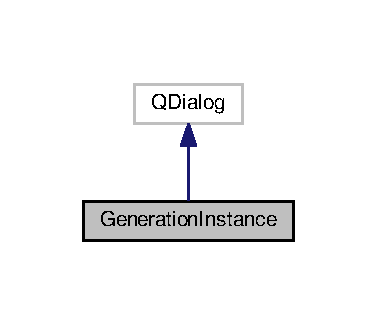
\includegraphics[width=181pt]{classGenerationInstance__inherit__graph}
\end{center}
\end{figure}


Collaboration diagram for Generation\+Instance\+:\nopagebreak
\begin{figure}[H]
\begin{center}
\leavevmode
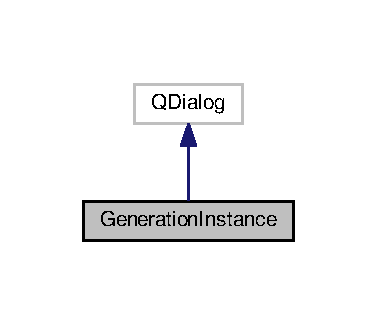
\includegraphics[width=181pt]{classGenerationInstance__coll__graph}
\end{center}
\end{figure}
\subsection*{Public Member Functions}
\begin{DoxyCompactItemize}
\item 
\hyperlink{classGenerationInstance_ac9c4a1ba1fe2f86209f116693f7c7b5b}{Generation\+Instance} (Q\+Widget $\ast$parent=0)
\begin{DoxyCompactList}\small\item\em Constructeur de la fenêtre \hyperlink{classGenerationInstance}{Generation\+Instance}. \end{DoxyCompactList}\item 
\hyperlink{classGenerationInstance_a14cdea0af4a47deb38a3a5fa59bb6d40}{$\sim$\+Generation\+Instance} ()
\begin{DoxyCompactList}\small\item\em Destructeur de la fenêtre \hyperlink{classGenerationInstance}{Generation\+Instance}. \end{DoxyCompactList}\item 
void \hyperlink{classGenerationInstance_a7e47ea4abf8249c100c253a142f9c5d0}{execution\+Generation\+Instance} (int nbr\+Instance, int nbr\+Jobs, int nbr\+Ressources, int nbr\+Machines, int horizon\+Planification)
\begin{DoxyCompactList}\small\item\em Fonction permetant d\textquotesingle{}executer la generation des instances spécifiées. \end{DoxyCompactList}\end{DoxyCompactItemize}


\subsection{Detailed Description}
La fenêtre de génération d\textquotesingle{}instance. 

\subsection{Constructor \& Destructor Documentation}
\mbox{\Hypertarget{classGenerationInstance_ac9c4a1ba1fe2f86209f116693f7c7b5b}\label{classGenerationInstance_ac9c4a1ba1fe2f86209f116693f7c7b5b}} 
\index{Generation\+Instance@{Generation\+Instance}!Generation\+Instance@{Generation\+Instance}}
\index{Generation\+Instance@{Generation\+Instance}!Generation\+Instance@{Generation\+Instance}}
\subsubsection{\texorpdfstring{Generation\+Instance()}{GenerationInstance()}}
{\footnotesize\ttfamily Generation\+Instance\+::\+Generation\+Instance (\begin{DoxyParamCaption}\item[{Q\+Widget $\ast$}]{parent = {\ttfamily 0} }\end{DoxyParamCaption})\hspace{0.3cm}{\ttfamily [explicit]}}



Constructeur de la fenêtre \hyperlink{classGenerationInstance}{Generation\+Instance}. 


\begin{DoxyParams}{Parameters}
{\em parent} & \\
\hline
\end{DoxyParams}
\mbox{\Hypertarget{classGenerationInstance_a14cdea0af4a47deb38a3a5fa59bb6d40}\label{classGenerationInstance_a14cdea0af4a47deb38a3a5fa59bb6d40}} 
\index{Generation\+Instance@{Generation\+Instance}!````~Generation\+Instance@{$\sim$\+Generation\+Instance}}
\index{````~Generation\+Instance@{$\sim$\+Generation\+Instance}!Generation\+Instance@{Generation\+Instance}}
\subsubsection{\texorpdfstring{$\sim$\+Generation\+Instance()}{~GenerationInstance()}}
{\footnotesize\ttfamily Generation\+Instance\+::$\sim$\+Generation\+Instance (\begin{DoxyParamCaption}{ }\end{DoxyParamCaption})}



Destructeur de la fenêtre \hyperlink{classGenerationInstance}{Generation\+Instance}. 

Here is the call graph for this function\+:\nopagebreak
\begin{figure}[H]
\begin{center}
\leavevmode
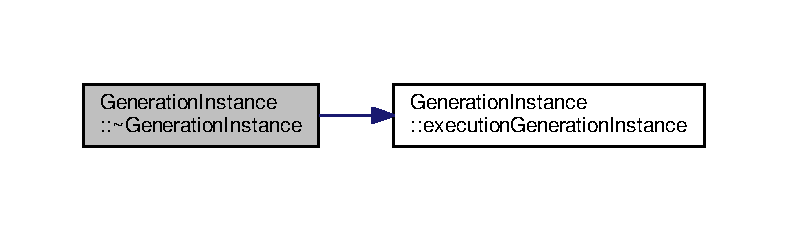
\includegraphics[width=350pt]{classGenerationInstance_a14cdea0af4a47deb38a3a5fa59bb6d40_cgraph}
\end{center}
\end{figure}


\subsection{Member Function Documentation}
\mbox{\Hypertarget{classGenerationInstance_a7e47ea4abf8249c100c253a142f9c5d0}\label{classGenerationInstance_a7e47ea4abf8249c100c253a142f9c5d0}} 
\index{Generation\+Instance@{Generation\+Instance}!execution\+Generation\+Instance@{execution\+Generation\+Instance}}
\index{execution\+Generation\+Instance@{execution\+Generation\+Instance}!Generation\+Instance@{Generation\+Instance}}
\subsubsection{\texorpdfstring{execution\+Generation\+Instance()}{executionGenerationInstance()}}
{\footnotesize\ttfamily void Generation\+Instance\+::execution\+Generation\+Instance (\begin{DoxyParamCaption}\item[{int}]{nbr\+Instance,  }\item[{int}]{nbr\+Jobs,  }\item[{int}]{nbr\+Ressources,  }\item[{int}]{nbr\+Machines,  }\item[{int}]{horizon\+Planification }\end{DoxyParamCaption})}



Fonction permetant d\textquotesingle{}executer la generation des instances spécifiées. 


\begin{DoxyParams}{Parameters}
{\em nbr\+Instance} & Le nombre d\textquotesingle{}instance à générer \\
\hline
{\em nbr\+Jobs} & Le nombre de jobs par instance \\
\hline
{\em nbr\+Ressources} & Le nombre de ressources par instance \\
\hline
{\em nbr\+Machines} & Le nombre de machines par instance \\
\hline
{\em horizon\+Planification} & L\textquotesingle{}horizon de planification maximale par instance \\
\hline
\end{DoxyParams}
Here is the caller graph for this function\+:\nopagebreak
\begin{figure}[H]
\begin{center}
\leavevmode
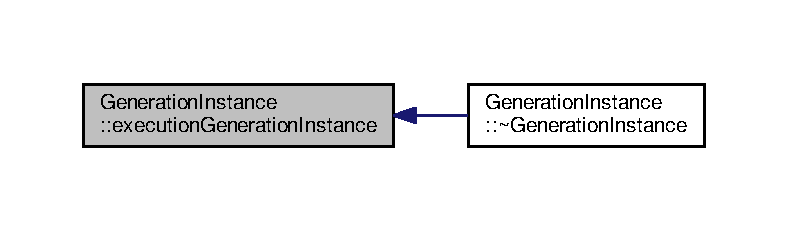
\includegraphics[width=350pt]{classGenerationInstance_a7e47ea4abf8249c100c253a142f9c5d0_icgraph}
\end{center}
\end{figure}


The documentation for this class was generated from the following files\+:\begin{DoxyCompactItemize}
\item 
P\+R\+D\+Ordonancement/\hyperlink{generationinstance_8h}{generationinstance.\+h}\item 
P\+R\+D\+Ordonancement/\hyperlink{generationinstance_8cpp}{generationinstance.\+cpp}\end{DoxyCompactItemize}

\hypertarget{classHeuristique}{}\section{Heuristique Class Reference}
\label{classHeuristique}\index{Heuristique@{Heuristique}}


Classe \hyperlink{classHeuristique}{Heuristique} permetant de trier et affecter des jobs sur des machines.  




{\ttfamily \#include $<$heuristique.\+h$>$}

\subsection*{Public Member Functions}
\begin{DoxyCompactItemize}
\item 
\hyperlink{classHeuristique_a58630433c6bac8eec9a5888945eba479}{Heuristique} (string fichier\+Instance)
\begin{DoxyCompactList}\small\item\em Constructeur de la classe \hyperlink{classHeuristique}{Heuristique}. \end{DoxyCompactList}\item 
vector$<$ int $>$ \hyperlink{classHeuristique_a19705558bc45437d88b750fe9cbe6125}{trier\+C\+Cmax\+Somme\+Ressources} ()
\begin{DoxyCompactList}\small\item\em Tri selon la méthode C\+Cmax basée sur la somme des ressources de chaque job. \end{DoxyCompactList}\item 
vector$<$ int $>$ \hyperlink{classHeuristique_a1fb7501d952a428b817ad179bc2a2185}{trier\+C\+Cmax\+Max\+Ressources} ()
\begin{DoxyCompactList}\small\item\em Tri selon la méthode C\+Cmax basée sur la valeur de ressource maximale de chaque job. \end{DoxyCompactList}\item 
vector$<$ int $>$ \hyperlink{classHeuristique_a019587ee3112631f8369d8ffe6303f2c}{trier\+Somme\+Ressources} ()
\begin{DoxyCompactList}\small\item\em Tri selon la somme des ressources de chaque job. \end{DoxyCompactList}\item 
vector$<$ int $>$ \hyperlink{classHeuristique_a9a5a00a6b2a9f0dc792491df1d7b6c67}{trier\+Moyenne\+Ressources\+Sous\+Ensembles} ()
\begin{DoxyCompactList}\small\item\em Tri selon la moyenne des ressources de chaque sous-\/ensembles maximaux de l\textquotesingle{}instance. \end{DoxyCompactList}\item 
map$<$ int, vector$<$ int $>$ $>$ \hyperlink{classHeuristique_a6799e05f33af7ac257ba56b9921a8baf}{get\+Sous\+Ensembles\+Maximaux} (vector$<$ vector$<$ int $>$$>$ eh, int nb\+\_\+job)
\begin{DoxyCompactList}\small\item\em Algorithme permetant de récupérer les sous-\/ensembles maximaux de l\textquotesingle{}instance. \end{DoxyCompactList}\item 
int \hyperlink{classHeuristique_a49b20cab1a9055fddf0519fe7bf99c4a}{resolve\+Machine\+Per\+Machine} (Q\+String type\+Tri, Q\+String fichier\+Resultat)
\begin{DoxyCompactList}\small\item\em Affectation machine par machine. \end{DoxyCompactList}\item 
int \hyperlink{classHeuristique_aa590500fc2368d1ea58ab483b2377fea}{resolve\+Machine\+Less\+Used\+Machine} (Q\+String type\+Tri, Q\+String fichier\+Resultat)
\begin{DoxyCompactList}\small\item\em Affectation privilégiant la machine la moins chargée. \end{DoxyCompactList}\item 
int \hyperlink{classHeuristique_adc1f4075bda4dfbf40f6ed4cc8a6c993}{write\+In\+File} (vector$<$ vector$<$ int $>$$>$ jobs\+Ordonnances, Q\+String type\+Resolution, Q\+String fichier\+Resultat, double duree\+Execution)
\begin{DoxyCompactList}\small\item\em Ecriture dans un fichier de résulat. \end{DoxyCompactList}\item 
\hyperlink{classInstance}{Instance} \hyperlink{classHeuristique_aa6eca6703702298968f03ac30c4be86f}{get\+Instance} () const
\begin{DoxyCompactList}\small\item\em Retourne l\textquotesingle{}instance courante. \end{DoxyCompactList}\item 
void \hyperlink{classHeuristique_a2b6477a1dde77d58415dd0bc75940352}{set\+Instance} (const \hyperlink{classInstance}{Instance} \&value)
\begin{DoxyCompactList}\small\item\em Permet de spécifier une instance. \end{DoxyCompactList}\end{DoxyCompactItemize}


\subsection{Detailed Description}
Classe \hyperlink{classHeuristique}{Heuristique} permetant de trier et affecter des jobs sur des machines. 

\subsection{Constructor \& Destructor Documentation}
\mbox{\Hypertarget{classHeuristique_a58630433c6bac8eec9a5888945eba479}\label{classHeuristique_a58630433c6bac8eec9a5888945eba479}} 
\index{Heuristique@{Heuristique}!Heuristique@{Heuristique}}
\index{Heuristique@{Heuristique}!Heuristique@{Heuristique}}
\subsubsection{\texorpdfstring{Heuristique()}{Heuristique()}}
{\footnotesize\ttfamily Heuristique\+::\+Heuristique (\begin{DoxyParamCaption}\item[{string}]{fichier\+Instance }\end{DoxyParamCaption})}



Constructeur de la classe \hyperlink{classHeuristique}{Heuristique}. 


\begin{DoxyParams}{Parameters}
{\em fichier\+Instance} & Le fichier d\textquotesingle{}instance \\
\hline
\end{DoxyParams}
Here is the call graph for this function\+:\nopagebreak
\begin{figure}[H]
\begin{center}
\leavevmode
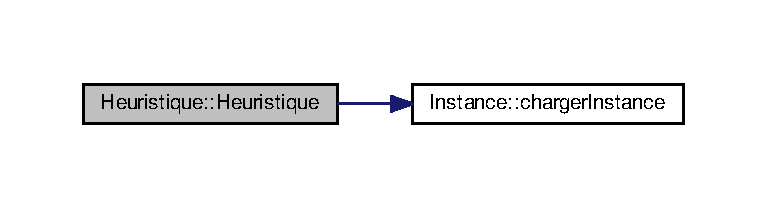
\includegraphics[width=350pt]{classHeuristique_a58630433c6bac8eec9a5888945eba479_cgraph}
\end{center}
\end{figure}


\subsection{Member Function Documentation}
\mbox{\Hypertarget{classHeuristique_aa6eca6703702298968f03ac30c4be86f}\label{classHeuristique_aa6eca6703702298968f03ac30c4be86f}} 
\index{Heuristique@{Heuristique}!get\+Instance@{get\+Instance}}
\index{get\+Instance@{get\+Instance}!Heuristique@{Heuristique}}
\subsubsection{\texorpdfstring{get\+Instance()}{getInstance()}}
{\footnotesize\ttfamily \hyperlink{classInstance}{Instance} Heuristique\+::get\+Instance (\begin{DoxyParamCaption}{ }\end{DoxyParamCaption}) const}



Retourne l\textquotesingle{}instance courante. 

\begin{DoxyReturn}{Returns}
\hyperlink{classInstance}{Instance} L\textquotesingle{}instance courante 
\end{DoxyReturn}
\mbox{\Hypertarget{classHeuristique_a6799e05f33af7ac257ba56b9921a8baf}\label{classHeuristique_a6799e05f33af7ac257ba56b9921a8baf}} 
\index{Heuristique@{Heuristique}!get\+Sous\+Ensembles\+Maximaux@{get\+Sous\+Ensembles\+Maximaux}}
\index{get\+Sous\+Ensembles\+Maximaux@{get\+Sous\+Ensembles\+Maximaux}!Heuristique@{Heuristique}}
\subsubsection{\texorpdfstring{get\+Sous\+Ensembles\+Maximaux()}{getSousEnsemblesMaximaux()}}
{\footnotesize\ttfamily map$<$ int, vector$<$ int $>$ $>$ Heuristique\+::get\+Sous\+Ensembles\+Maximaux (\begin{DoxyParamCaption}\item[{vector$<$ vector$<$ int $>$$>$}]{eh,  }\item[{int}]{nb\+\_\+job }\end{DoxyParamCaption})}



Algorithme permetant de récupérer les sous-\/ensembles maximaux de l\textquotesingle{}instance. 


\begin{DoxyParams}{Parameters}
{\em eh} & La liste d\textquotesingle{}événement classée \\
\hline
{\em nb\+\_\+job} & Le nombre de jobs de l\textquotesingle{}instance \\
\hline
\end{DoxyParams}
\begin{DoxyReturn}{Returns}
map$<$int, vector$<$int$>$ $>$ Les sous ensembles maximaux 
\end{DoxyReturn}
Here is the caller graph for this function\+:\nopagebreak
\begin{figure}[H]
\begin{center}
\leavevmode
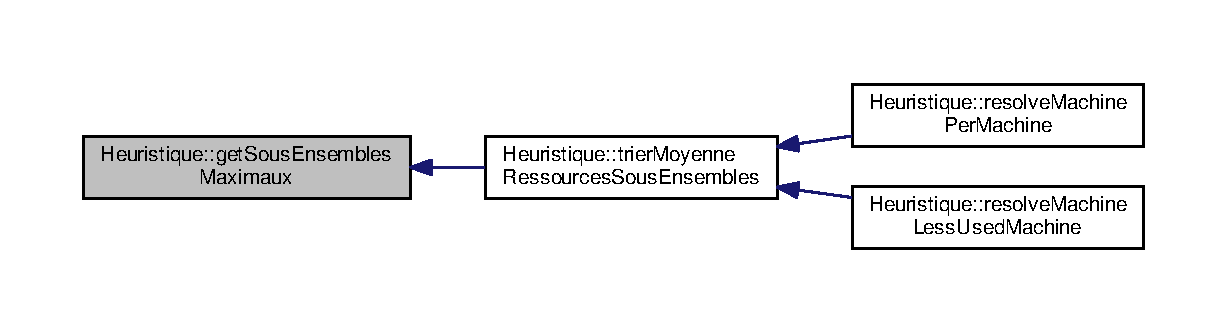
\includegraphics[width=350pt]{classHeuristique_a6799e05f33af7ac257ba56b9921a8baf_icgraph}
\end{center}
\end{figure}
\mbox{\Hypertarget{classHeuristique_aa590500fc2368d1ea58ab483b2377fea}\label{classHeuristique_aa590500fc2368d1ea58ab483b2377fea}} 
\index{Heuristique@{Heuristique}!resolve\+Machine\+Less\+Used\+Machine@{resolve\+Machine\+Less\+Used\+Machine}}
\index{resolve\+Machine\+Less\+Used\+Machine@{resolve\+Machine\+Less\+Used\+Machine}!Heuristique@{Heuristique}}
\subsubsection{\texorpdfstring{resolve\+Machine\+Less\+Used\+Machine()}{resolveMachineLessUsedMachine()}}
{\footnotesize\ttfamily int Heuristique\+::resolve\+Machine\+Less\+Used\+Machine (\begin{DoxyParamCaption}\item[{Q\+String}]{type\+Tri,  }\item[{Q\+String}]{fichier\+Resultat }\end{DoxyParamCaption})}



Affectation privilégiant la machine la moins chargée. 


\begin{DoxyParams}{Parameters}
{\em type\+Tri} & Le type de tri à utiliser avant l\textquotesingle{}affectation \\
\hline
{\em fichier\+Resultat} & Le fichier où seront stockés les résulats \\
\hline
\end{DoxyParams}
\begin{DoxyReturn}{Returns}
int Le nombre de jobs ordonnancés 
\end{DoxyReturn}
Here is the call graph for this function\+:\nopagebreak
\begin{figure}[H]
\begin{center}
\leavevmode
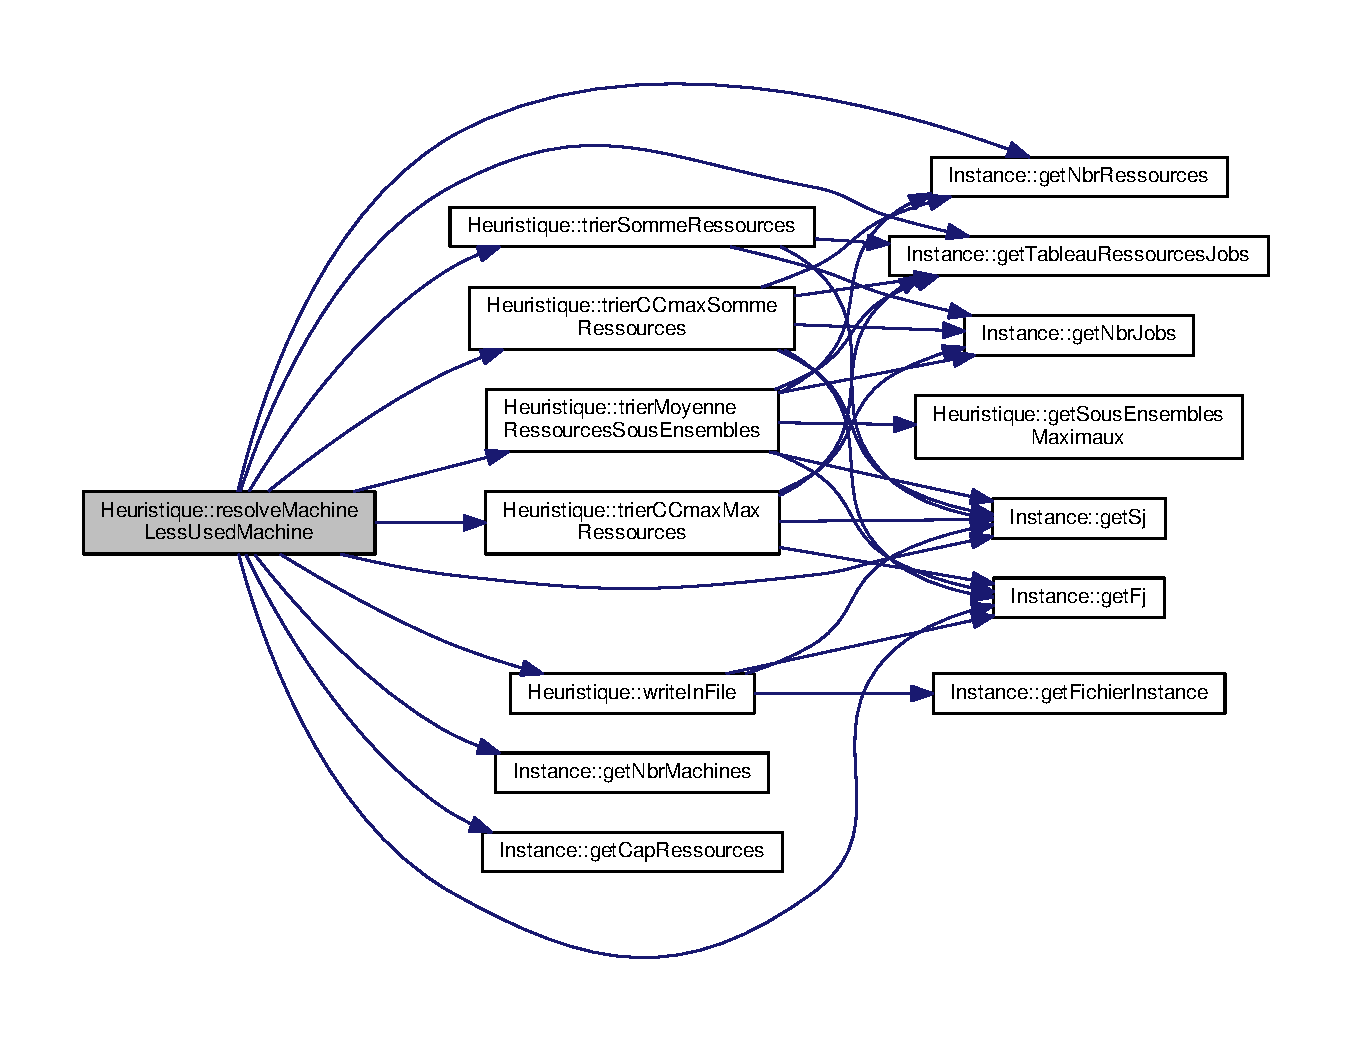
\includegraphics[width=350pt]{classHeuristique_aa590500fc2368d1ea58ab483b2377fea_cgraph}
\end{center}
\end{figure}
\mbox{\Hypertarget{classHeuristique_a49b20cab1a9055fddf0519fe7bf99c4a}\label{classHeuristique_a49b20cab1a9055fddf0519fe7bf99c4a}} 
\index{Heuristique@{Heuristique}!resolve\+Machine\+Per\+Machine@{resolve\+Machine\+Per\+Machine}}
\index{resolve\+Machine\+Per\+Machine@{resolve\+Machine\+Per\+Machine}!Heuristique@{Heuristique}}
\subsubsection{\texorpdfstring{resolve\+Machine\+Per\+Machine()}{resolveMachinePerMachine()}}
{\footnotesize\ttfamily int Heuristique\+::resolve\+Machine\+Per\+Machine (\begin{DoxyParamCaption}\item[{Q\+String}]{type\+Tri,  }\item[{Q\+String}]{fichier\+Resultat }\end{DoxyParamCaption})}



Affectation machine par machine. 


\begin{DoxyParams}{Parameters}
{\em type\+Tri} & Le type de tri à utiliser avant l\textquotesingle{}affectation \\
\hline
{\em fichier\+Resultat} & Le fichier où seront stockés les résulats \\
\hline
\end{DoxyParams}
\begin{DoxyReturn}{Returns}
int Le nombre de jobs ordonnancés 
\end{DoxyReturn}
Here is the call graph for this function\+:\nopagebreak
\begin{figure}[H]
\begin{center}
\leavevmode
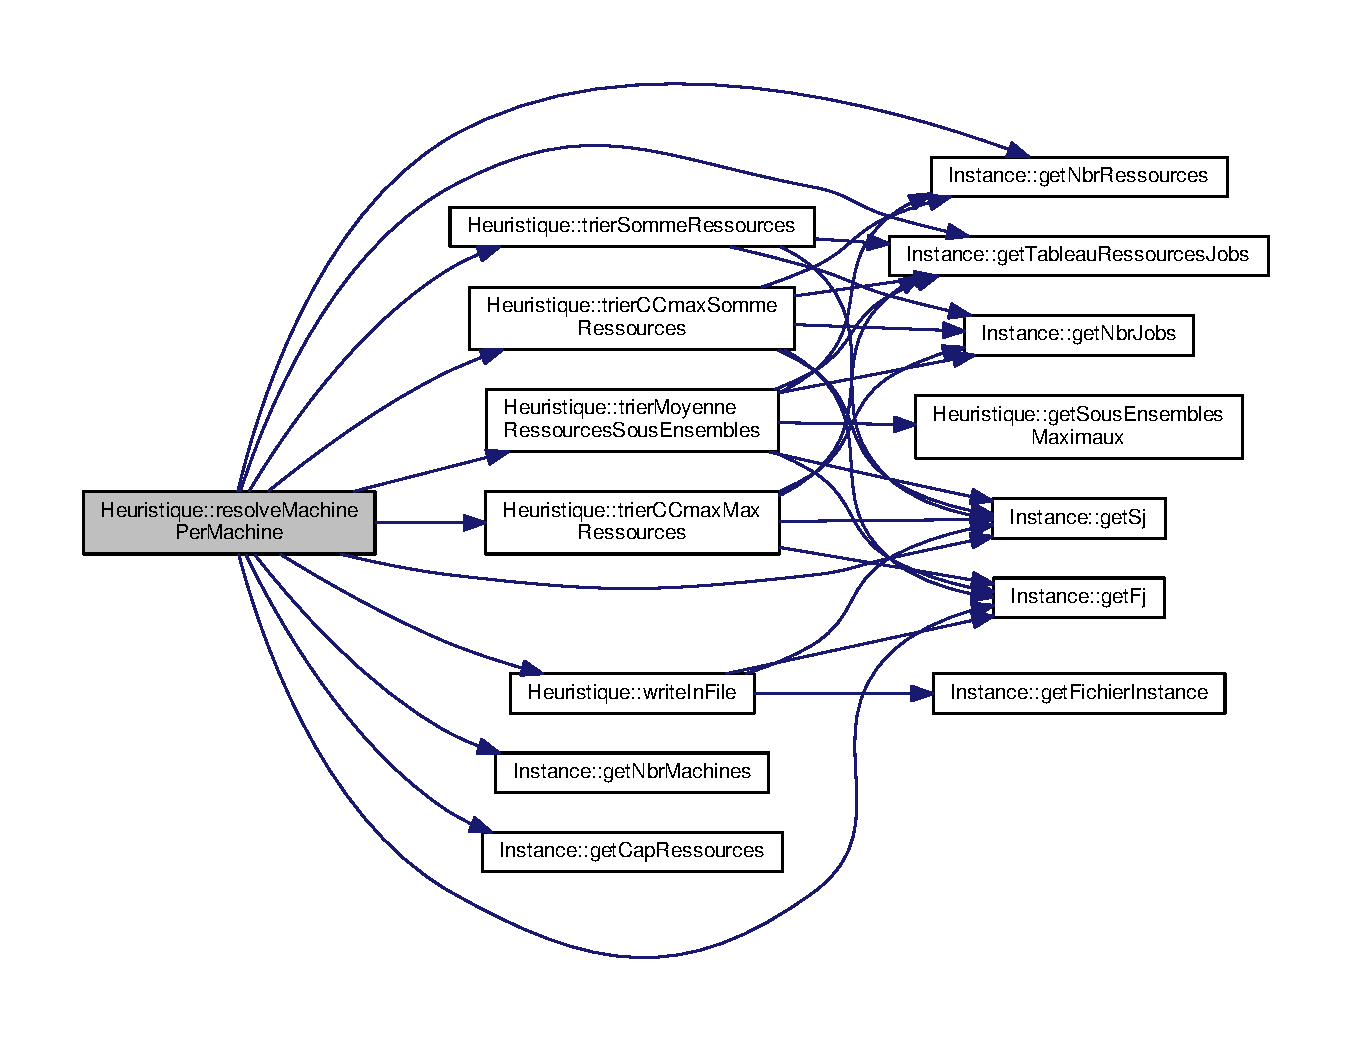
\includegraphics[width=350pt]{classHeuristique_a49b20cab1a9055fddf0519fe7bf99c4a_cgraph}
\end{center}
\end{figure}
\mbox{\Hypertarget{classHeuristique_a2b6477a1dde77d58415dd0bc75940352}\label{classHeuristique_a2b6477a1dde77d58415dd0bc75940352}} 
\index{Heuristique@{Heuristique}!set\+Instance@{set\+Instance}}
\index{set\+Instance@{set\+Instance}!Heuristique@{Heuristique}}
\subsubsection{\texorpdfstring{set\+Instance()}{setInstance()}}
{\footnotesize\ttfamily void Heuristique\+::set\+Instance (\begin{DoxyParamCaption}\item[{const \hyperlink{classInstance}{Instance} \&}]{value }\end{DoxyParamCaption})}



Permet de spécifier une instance. 


\begin{DoxyParams}{Parameters}
{\em value} & L\textquotesingle{}instance que l\textquotesingle{}on souhaite spécifier \\
\hline
\end{DoxyParams}
\mbox{\Hypertarget{classHeuristique_a1fb7501d952a428b817ad179bc2a2185}\label{classHeuristique_a1fb7501d952a428b817ad179bc2a2185}} 
\index{Heuristique@{Heuristique}!trier\+C\+Cmax\+Max\+Ressources@{trier\+C\+Cmax\+Max\+Ressources}}
\index{trier\+C\+Cmax\+Max\+Ressources@{trier\+C\+Cmax\+Max\+Ressources}!Heuristique@{Heuristique}}
\subsubsection{\texorpdfstring{trier\+C\+Cmax\+Max\+Ressources()}{trierCCmaxMaxRessources()}}
{\footnotesize\ttfamily vector$<$ int $>$ Heuristique\+::trier\+C\+Cmax\+Max\+Ressources (\begin{DoxyParamCaption}{ }\end{DoxyParamCaption})}



Tri selon la méthode C\+Cmax basée sur la valeur de ressource maximale de chaque job. 

\begin{DoxyReturn}{Returns}
vector$<$int$>$ La liste des jobs triés 
\end{DoxyReturn}
Here is the call graph for this function\+:\nopagebreak
\begin{figure}[H]
\begin{center}
\leavevmode
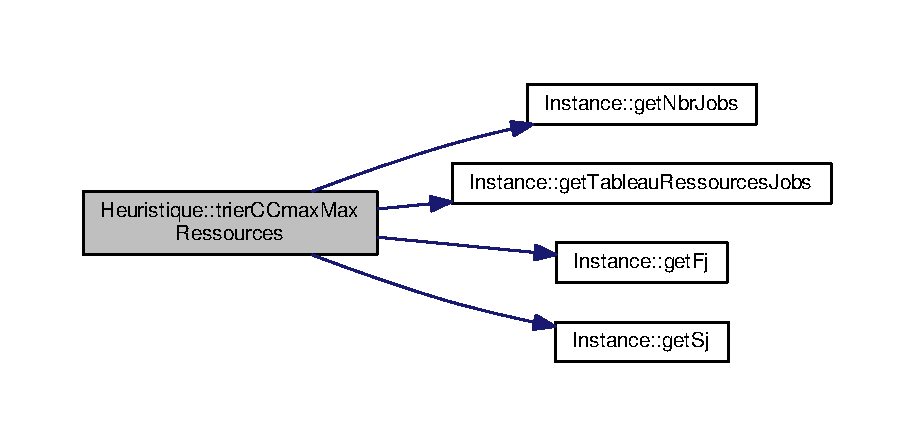
\includegraphics[width=350pt]{classHeuristique_a1fb7501d952a428b817ad179bc2a2185_cgraph}
\end{center}
\end{figure}
Here is the caller graph for this function\+:\nopagebreak
\begin{figure}[H]
\begin{center}
\leavevmode
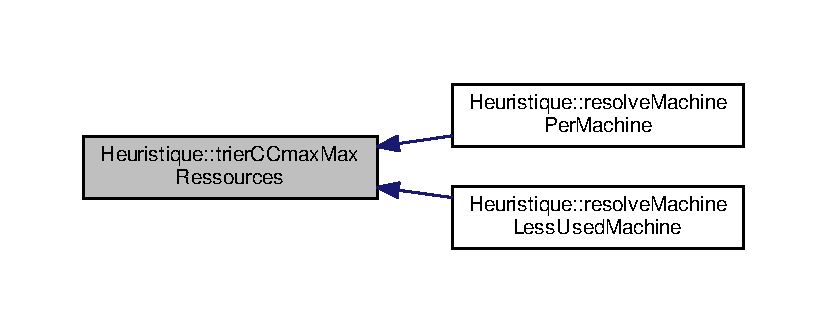
\includegraphics[width=350pt]{classHeuristique_a1fb7501d952a428b817ad179bc2a2185_icgraph}
\end{center}
\end{figure}
\mbox{\Hypertarget{classHeuristique_a19705558bc45437d88b750fe9cbe6125}\label{classHeuristique_a19705558bc45437d88b750fe9cbe6125}} 
\index{Heuristique@{Heuristique}!trier\+C\+Cmax\+Somme\+Ressources@{trier\+C\+Cmax\+Somme\+Ressources}}
\index{trier\+C\+Cmax\+Somme\+Ressources@{trier\+C\+Cmax\+Somme\+Ressources}!Heuristique@{Heuristique}}
\subsubsection{\texorpdfstring{trier\+C\+Cmax\+Somme\+Ressources()}{trierCCmaxSommeRessources()}}
{\footnotesize\ttfamily vector$<$ int $>$ Heuristique\+::trier\+C\+Cmax\+Somme\+Ressources (\begin{DoxyParamCaption}{ }\end{DoxyParamCaption})}



Tri selon la méthode C\+Cmax basée sur la somme des ressources de chaque job. 

\begin{DoxyReturn}{Returns}
vector$<$int$>$ La liste des jobs triés 
\end{DoxyReturn}
Here is the call graph for this function\+:\nopagebreak
\begin{figure}[H]
\begin{center}
\leavevmode
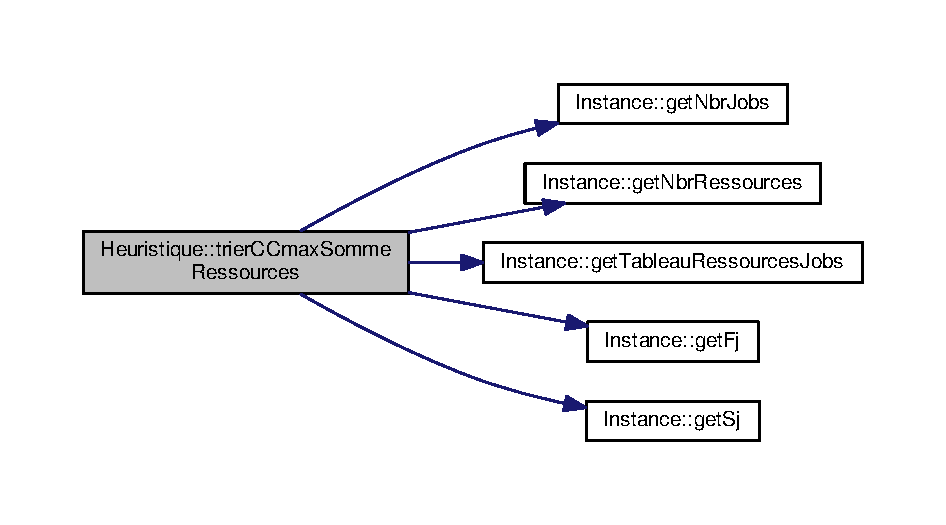
\includegraphics[width=350pt]{classHeuristique_a19705558bc45437d88b750fe9cbe6125_cgraph}
\end{center}
\end{figure}
Here is the caller graph for this function\+:\nopagebreak
\begin{figure}[H]
\begin{center}
\leavevmode
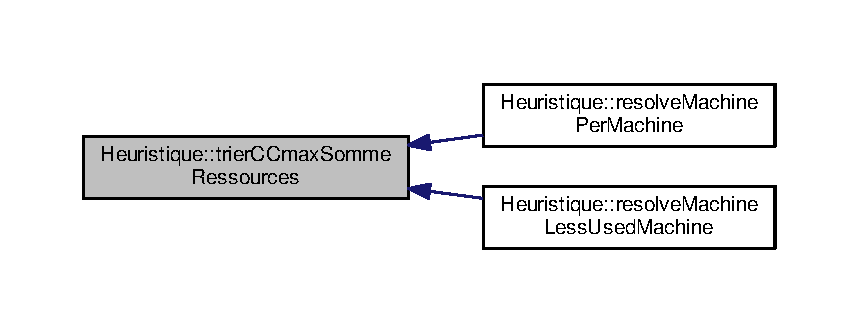
\includegraphics[width=350pt]{classHeuristique_a19705558bc45437d88b750fe9cbe6125_icgraph}
\end{center}
\end{figure}
\mbox{\Hypertarget{classHeuristique_a9a5a00a6b2a9f0dc792491df1d7b6c67}\label{classHeuristique_a9a5a00a6b2a9f0dc792491df1d7b6c67}} 
\index{Heuristique@{Heuristique}!trier\+Moyenne\+Ressources\+Sous\+Ensembles@{trier\+Moyenne\+Ressources\+Sous\+Ensembles}}
\index{trier\+Moyenne\+Ressources\+Sous\+Ensembles@{trier\+Moyenne\+Ressources\+Sous\+Ensembles}!Heuristique@{Heuristique}}
\subsubsection{\texorpdfstring{trier\+Moyenne\+Ressources\+Sous\+Ensembles()}{trierMoyenneRessourcesSousEnsembles()}}
{\footnotesize\ttfamily vector$<$ int $>$ Heuristique\+::trier\+Moyenne\+Ressources\+Sous\+Ensembles (\begin{DoxyParamCaption}{ }\end{DoxyParamCaption})}



Tri selon la moyenne des ressources de chaque sous-\/ensembles maximaux de l\textquotesingle{}instance. 

\begin{DoxyReturn}{Returns}
vector$<$int$>$ La liste des jobs triés 
\end{DoxyReturn}
Here is the call graph for this function\+:\nopagebreak
\begin{figure}[H]
\begin{center}
\leavevmode
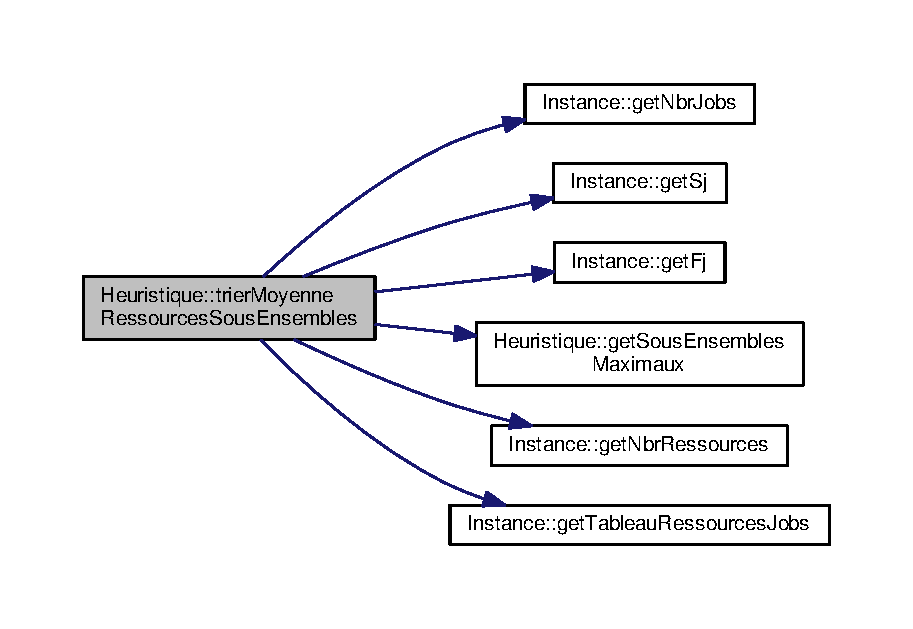
\includegraphics[width=350pt]{classHeuristique_a9a5a00a6b2a9f0dc792491df1d7b6c67_cgraph}
\end{center}
\end{figure}
Here is the caller graph for this function\+:\nopagebreak
\begin{figure}[H]
\begin{center}
\leavevmode
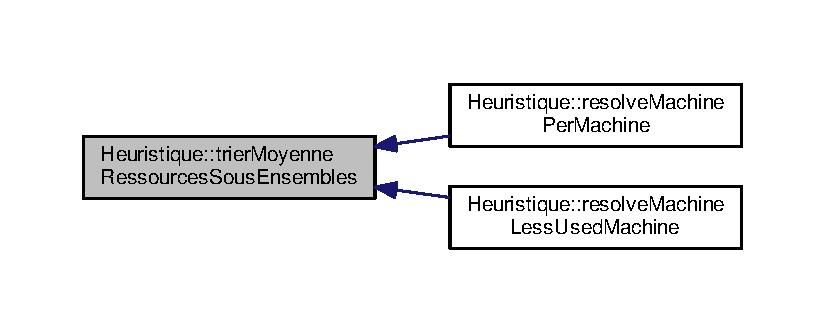
\includegraphics[width=350pt]{classHeuristique_a9a5a00a6b2a9f0dc792491df1d7b6c67_icgraph}
\end{center}
\end{figure}
\mbox{\Hypertarget{classHeuristique_a019587ee3112631f8369d8ffe6303f2c}\label{classHeuristique_a019587ee3112631f8369d8ffe6303f2c}} 
\index{Heuristique@{Heuristique}!trier\+Somme\+Ressources@{trier\+Somme\+Ressources}}
\index{trier\+Somme\+Ressources@{trier\+Somme\+Ressources}!Heuristique@{Heuristique}}
\subsubsection{\texorpdfstring{trier\+Somme\+Ressources()}{trierSommeRessources()}}
{\footnotesize\ttfamily vector$<$ int $>$ Heuristique\+::trier\+Somme\+Ressources (\begin{DoxyParamCaption}{ }\end{DoxyParamCaption})}



Tri selon la somme des ressources de chaque job. 

\begin{DoxyReturn}{Returns}
vector$<$int$>$ La liste des jobs triés 
\end{DoxyReturn}
Here is the call graph for this function\+:\nopagebreak
\begin{figure}[H]
\begin{center}
\leavevmode
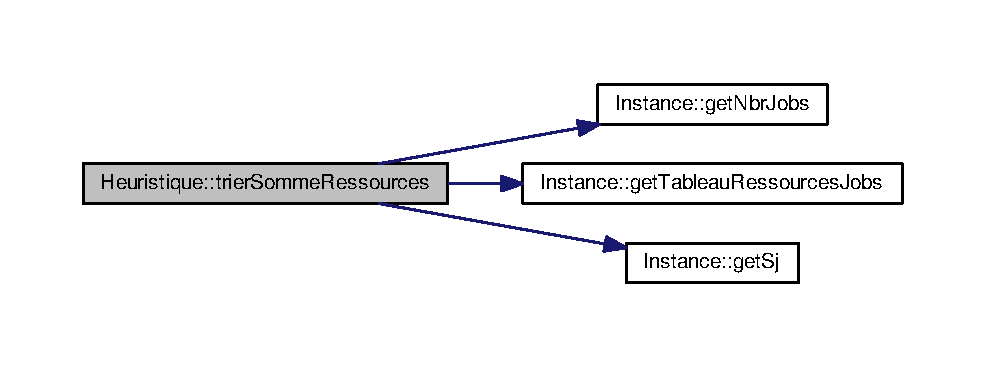
\includegraphics[width=350pt]{classHeuristique_a019587ee3112631f8369d8ffe6303f2c_cgraph}
\end{center}
\end{figure}
Here is the caller graph for this function\+:\nopagebreak
\begin{figure}[H]
\begin{center}
\leavevmode
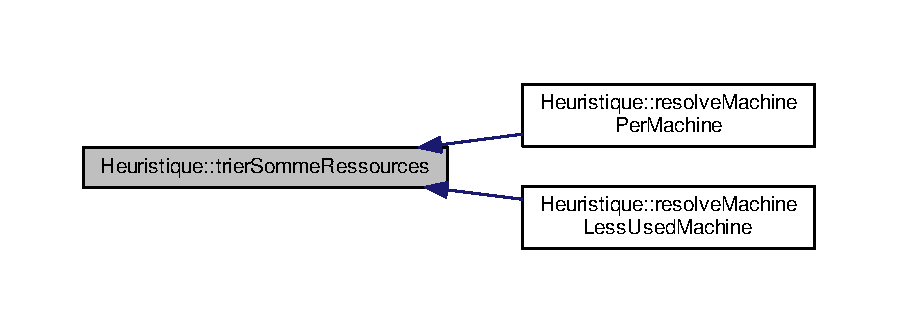
\includegraphics[width=350pt]{classHeuristique_a019587ee3112631f8369d8ffe6303f2c_icgraph}
\end{center}
\end{figure}
\mbox{\Hypertarget{classHeuristique_adc1f4075bda4dfbf40f6ed4cc8a6c993}\label{classHeuristique_adc1f4075bda4dfbf40f6ed4cc8a6c993}} 
\index{Heuristique@{Heuristique}!write\+In\+File@{write\+In\+File}}
\index{write\+In\+File@{write\+In\+File}!Heuristique@{Heuristique}}
\subsubsection{\texorpdfstring{write\+In\+File()}{writeInFile()}}
{\footnotesize\ttfamily int Heuristique\+::write\+In\+File (\begin{DoxyParamCaption}\item[{vector$<$ vector$<$ int $>$$>$}]{jobs\+Ordonnances,  }\item[{Q\+String}]{type\+Resolution,  }\item[{Q\+String}]{fichier\+Resultat,  }\item[{double}]{duree\+Execution }\end{DoxyParamCaption})}



Ecriture dans un fichier de résulat. 


\begin{DoxyParams}{Parameters}
{\em jobs\+Ordonnances} & Le tableau de jobs ordonancés \\
\hline
{\em type\+Resolution} & Le type de résolution \\
\hline
{\em fichier\+Resultat} & Le fichier où seront stockés les résulats \\
\hline
{\em duree\+Execution} & La durée d\textquotesingle{}execution de la résolution \\
\hline
\end{DoxyParams}
\begin{DoxyReturn}{Returns}
int Le nombre de jobs ordonnancés 
\end{DoxyReturn}
Here is the call graph for this function\+:\nopagebreak
\begin{figure}[H]
\begin{center}
\leavevmode
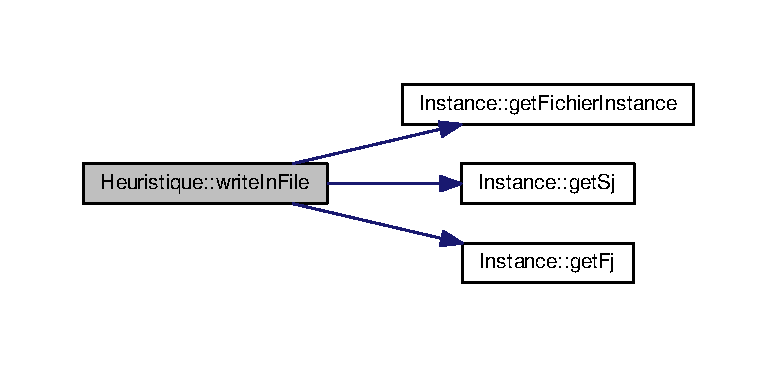
\includegraphics[width=350pt]{classHeuristique_adc1f4075bda4dfbf40f6ed4cc8a6c993_cgraph}
\end{center}
\end{figure}
Here is the caller graph for this function\+:\nopagebreak
\begin{figure}[H]
\begin{center}
\leavevmode
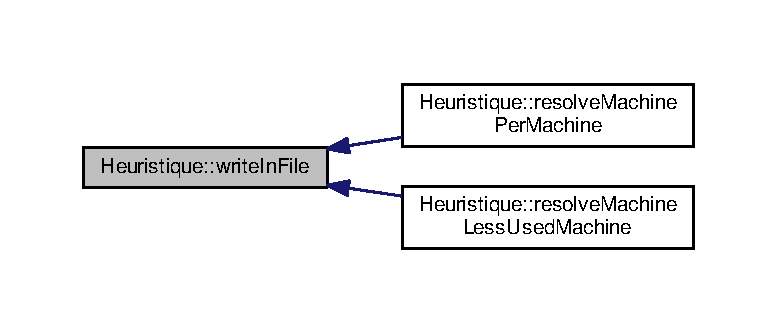
\includegraphics[width=350pt]{classHeuristique_adc1f4075bda4dfbf40f6ed4cc8a6c993_icgraph}
\end{center}
\end{figure}


The documentation for this class was generated from the following files\+:\begin{DoxyCompactItemize}
\item 
P\+R\+D\+Ordonancement/\hyperlink{heuristique_8h}{heuristique.\+h}\item 
P\+R\+D\+Ordonancement/\hyperlink{heuristique_8cpp}{heuristique.\+cpp}\end{DoxyCompactItemize}

\hypertarget{classInstance}{}\section{Instance Class Reference}
\label{classInstance}\index{Instance@{Instance}}


Classe représentant une instance.  




{\ttfamily \#include $<$instance.\+h$>$}

\subsection*{Public Member Functions}
\begin{DoxyCompactItemize}
\item 
\hyperlink{classInstance_a399506c7e75ab9ab78fbc34a25932bbd}{Instance} ()
\begin{DoxyCompactList}\small\item\em Constructeur de la classe \hyperlink{classInstance}{Instance}. \end{DoxyCompactList}\item 
Q\+String \hyperlink{classInstance_a783365375cdab53149f87208374331a7}{get\+Fichier\+Instance} () const
\begin{DoxyCompactList}\small\item\em Permet de retourner le chemin vers le fichier d\textquotesingle{}instance. \end{DoxyCompactList}\item 
void \hyperlink{classInstance_a263461a7a8c44c9e7080620a30cc8fcf}{set\+Fichier\+Instance} (const Q\+String \&value)
\begin{DoxyCompactList}\small\item\em Setter du chemin vers le fichier d\textquotesingle{}instance. \end{DoxyCompactList}\item 
unsigned int \hyperlink{classInstance_a1ed694b05c888cdb177ddf4c92a482d9}{get\+Nbr\+Jobs} () const
\begin{DoxyCompactList}\small\item\em Permet d\textquotesingle{}obtenir le nombre de jobs de l\textquotesingle{}instance. \end{DoxyCompactList}\item 
void \hyperlink{classInstance_ade6c7b12ee34960cebb060d669ec8f06}{set\+Nbr\+Jobs} (unsigned int value)
\begin{DoxyCompactList}\small\item\em Setter du nombre de jobs de l\textquotesingle{}instance. \end{DoxyCompactList}\item 
unsigned int \hyperlink{classInstance_a79b49dcc3d590b823e41d8a223ecf25d}{get\+Nbr\+Ressources} () const
\begin{DoxyCompactList}\small\item\em Permet d\textquotesingle{}obtenir le nombre de ressources de l\textquotesingle{}instance. \end{DoxyCompactList}\item 
void \hyperlink{classInstance_aefc2e4c0a18ad899f99cad856a749358}{set\+Nbr\+Ressources} (unsigned int value)
\begin{DoxyCompactList}\small\item\em Setter du nombre de ressources de l\textquotesingle{}instance. \end{DoxyCompactList}\item 
unsigned int \hyperlink{classInstance_a2f985b9a7ce18fd8739ec589d9016003}{get\+Nbr\+Machines} () const
\begin{DoxyCompactList}\small\item\em Permet d\textquotesingle{}obtenir le nombre de machines de l\textquotesingle{}instance. \end{DoxyCompactList}\item 
void \hyperlink{classInstance_a7087e8d1d2a5a4d275472dc908a06381}{set\+Nbr\+Machines} (unsigned int value)
\begin{DoxyCompactList}\small\item\em Setter du nombre de machines de l\textquotesingle{}instance. \end{DoxyCompactList}\item 
vector$<$ unsigned int $>$ \hyperlink{classInstance_ab998bc8d9a8b03c8f6279573779217cc}{get\+Sj} () const
\begin{DoxyCompactList}\small\item\em Permet d\textquotesingle{}obtenir le tableau des instants de départ de l\textquotesingle{}ensemble des jobs. \end{DoxyCompactList}\item 
void \hyperlink{classInstance_af695a8a91368f2484ee7367b14144742}{set\+Sj} (const vector$<$ unsigned int $>$ \&value)
\begin{DoxyCompactList}\small\item\em Setter du tableau des instants de départ de l\textquotesingle{}ensemble des jobs. \end{DoxyCompactList}\item 
vector$<$ unsigned int $>$ \hyperlink{classInstance_af7b70cbd8670e4eb213fbd2b81eca6f0}{get\+Fj} () const
\begin{DoxyCompactList}\small\item\em Permet d\textquotesingle{}obtenir le tableau des instants de fin de l\textquotesingle{}ensemble des jobs. \end{DoxyCompactList}\item 
void \hyperlink{classInstance_a544764ab0dcb42e795c5bfee4a0681cf}{set\+Fj} (const vector$<$ unsigned int $>$ \&value)
\begin{DoxyCompactList}\small\item\em Setter du tableau des instants de fin de l\textquotesingle{}ensemble des jobs. \end{DoxyCompactList}\item 
vector$<$ vector$<$ unsigned int $>$ $>$ \hyperlink{classInstance_a5dac330671540cf94e87b7586cd3102e}{get\+Cap\+Ressources} () const
\begin{DoxyCompactList}\small\item\em Permet d\textquotesingle{}obtenir le tableau des capacités en ressource pour l\textquotesingle{}ensemble des machines. \end{DoxyCompactList}\item 
void \hyperlink{classInstance_a527d6a6623e0257f4512a96285a960a5}{set\+Cap\+Ressources} (const vector$<$ vector$<$ unsigned int $>$$>$ \&value)
\begin{DoxyCompactList}\small\item\em Setter du tableau des capacités en ressource pour l\textquotesingle{}ensemble des machines. \end{DoxyCompactList}\item 
vector$<$ vector$<$ unsigned int $>$ $>$ \hyperlink{classInstance_ad4124bd2f1edb83a46ef94cfe07eafc8}{get\+Tableau\+Ressources\+Jobs} () const
\begin{DoxyCompactList}\small\item\em Permet d\textquotesingle{}obtenir le tableau des capacités en ressource pour l\textquotesingle{}ensemble des jobs. \end{DoxyCompactList}\item 
void \hyperlink{classInstance_a702ba79351487440788af8d662f1266c}{set\+Tableau\+Ressources\+Jobs} (const vector$<$ vector$<$ unsigned int $>$ $>$ \&value)
\begin{DoxyCompactList}\small\item\em Setter du tableau des capacités en ressource pour l\textquotesingle{}ensemble des jobs. \end{DoxyCompactList}\item 
unsigned int \hyperlink{classInstance_a8bf10528309a62149cc188dd2b80f0b7}{get\+Horizon\+Max} () const
\begin{DoxyCompactList}\small\item\em Permet d\textquotesingle{}obtenir l\textquotesingle{}horizon maximale de planification de l\textquotesingle{}instance. \end{DoxyCompactList}\item 
void \hyperlink{classInstance_aca68cfedc71eb3b2e7051ef99412e965}{set\+Horizon\+Max} (unsigned int value)
\begin{DoxyCompactList}\small\item\em Setter de l\textquotesingle{}horizon maximale de planification de l\textquotesingle{}instance. \end{DoxyCompactList}\item 
void \hyperlink{classInstance_aa64eca6a12ffa8ffc850ac4e04f268fb}{charger\+Instance} (string fichier\+Instance)
\begin{DoxyCompactList}\small\item\em Permet de charger une instance à partir d\textquotesingle{}un chemin vers un fichier d\textquotesingle{}instance. \end{DoxyCompactList}\item 
map$<$ unsigned int, vector$<$ unsigned int $>$ $>$ \hyperlink{classInstance_a2011ff3253fcb1d2d354c3c34a14a6fb}{get\+Sous\+Ensembles\+Maximaux} ()
\begin{DoxyCompactList}\small\item\em Retourne les sous-\/ensembles maximaux de jobs de l\textquotesingle{}instance (jobs se chevauchant) \end{DoxyCompactList}\item 
void \hyperlink{classInstance_a36e8de8c42d48f16f14f37622dbd3eb1}{sauvegarder\+Instance} (unsigned int nbr\+Instance, unsigned int nbr\+Jobs, unsigned int nbr\+Ressources, unsigned int nbr\+Machines, unsigned int horizon\+Planification)
\begin{DoxyCompactList}\small\item\em Permet de sauvegarder des instances avec des paramètres particuliers. \end{DoxyCompactList}\end{DoxyCompactItemize}


\subsection{Detailed Description}
Classe représentant une instance. 

\subsection{Constructor \& Destructor Documentation}
\mbox{\Hypertarget{classInstance_a399506c7e75ab9ab78fbc34a25932bbd}\label{classInstance_a399506c7e75ab9ab78fbc34a25932bbd}} 
\index{Instance@{Instance}!Instance@{Instance}}
\index{Instance@{Instance}!Instance@{Instance}}
\subsubsection{\texorpdfstring{Instance()}{Instance()}}
{\footnotesize\ttfamily Instance\+::\+Instance (\begin{DoxyParamCaption}{ }\end{DoxyParamCaption})}



Constructeur de la classe \hyperlink{classInstance}{Instance}. 



\subsection{Member Function Documentation}
\mbox{\Hypertarget{classInstance_aa64eca6a12ffa8ffc850ac4e04f268fb}\label{classInstance_aa64eca6a12ffa8ffc850ac4e04f268fb}} 
\index{Instance@{Instance}!charger\+Instance@{charger\+Instance}}
\index{charger\+Instance@{charger\+Instance}!Instance@{Instance}}
\subsubsection{\texorpdfstring{charger\+Instance()}{chargerInstance()}}
{\footnotesize\ttfamily void Instance\+::charger\+Instance (\begin{DoxyParamCaption}\item[{string}]{fichier\+Instance }\end{DoxyParamCaption})}



Permet de charger une instance à partir d\textquotesingle{}un chemin vers un fichier d\textquotesingle{}instance. 


\begin{DoxyParams}{Parameters}
{\em fichier\+Instance} & Le chemin vers le fichier d\textquotesingle{}instance \\
\hline
\end{DoxyParams}
Here is the caller graph for this function\+:\nopagebreak
\begin{figure}[H]
\begin{center}
\leavevmode
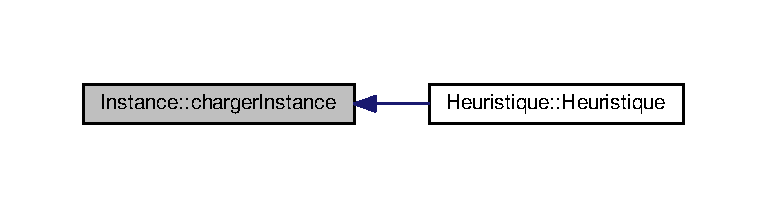
\includegraphics[width=350pt]{classInstance_aa64eca6a12ffa8ffc850ac4e04f268fb_icgraph}
\end{center}
\end{figure}
\mbox{\Hypertarget{classInstance_a5dac330671540cf94e87b7586cd3102e}\label{classInstance_a5dac330671540cf94e87b7586cd3102e}} 
\index{Instance@{Instance}!get\+Cap\+Ressources@{get\+Cap\+Ressources}}
\index{get\+Cap\+Ressources@{get\+Cap\+Ressources}!Instance@{Instance}}
\subsubsection{\texorpdfstring{get\+Cap\+Ressources()}{getCapRessources()}}
{\footnotesize\ttfamily vector$<$ vector$<$ unsigned int $>$ $>$ Instance\+::get\+Cap\+Ressources (\begin{DoxyParamCaption}{ }\end{DoxyParamCaption}) const}



Permet d\textquotesingle{}obtenir le tableau des capacités en ressource pour l\textquotesingle{}ensemble des machines. 

\begin{DoxyReturn}{Returns}
vector$<$vector$<$unsigned int$>$$>$ Le tableau des capacités en ressource pour l\textquotesingle{}ensemble des machines 
\end{DoxyReturn}
Here is the caller graph for this function\+:\nopagebreak
\begin{figure}[H]
\begin{center}
\leavevmode
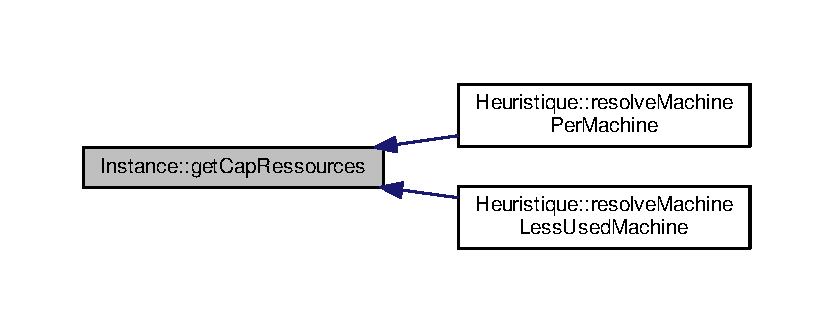
\includegraphics[width=350pt]{classInstance_a5dac330671540cf94e87b7586cd3102e_icgraph}
\end{center}
\end{figure}
\mbox{\Hypertarget{classInstance_a783365375cdab53149f87208374331a7}\label{classInstance_a783365375cdab53149f87208374331a7}} 
\index{Instance@{Instance}!get\+Fichier\+Instance@{get\+Fichier\+Instance}}
\index{get\+Fichier\+Instance@{get\+Fichier\+Instance}!Instance@{Instance}}
\subsubsection{\texorpdfstring{get\+Fichier\+Instance()}{getFichierInstance()}}
{\footnotesize\ttfamily Q\+String Instance\+::get\+Fichier\+Instance (\begin{DoxyParamCaption}{ }\end{DoxyParamCaption}) const}



Permet de retourner le chemin vers le fichier d\textquotesingle{}instance. 

\begin{DoxyReturn}{Returns}
Q\+String Le chemin vers le fichier d\textquotesingle{}instance 
\end{DoxyReturn}
Here is the caller graph for this function\+:\nopagebreak
\begin{figure}[H]
\begin{center}
\leavevmode
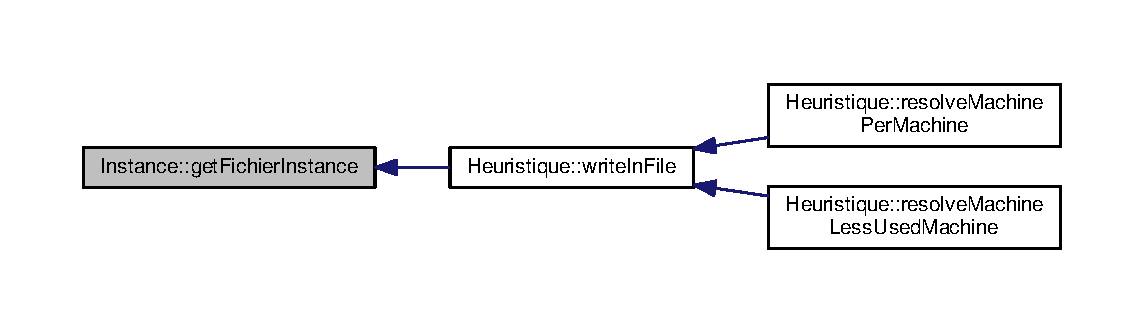
\includegraphics[width=350pt]{classInstance_a783365375cdab53149f87208374331a7_icgraph}
\end{center}
\end{figure}
\mbox{\Hypertarget{classInstance_af7b70cbd8670e4eb213fbd2b81eca6f0}\label{classInstance_af7b70cbd8670e4eb213fbd2b81eca6f0}} 
\index{Instance@{Instance}!get\+Fj@{get\+Fj}}
\index{get\+Fj@{get\+Fj}!Instance@{Instance}}
\subsubsection{\texorpdfstring{get\+Fj()}{getFj()}}
{\footnotesize\ttfamily vector$<$ unsigned int $>$ Instance\+::get\+Fj (\begin{DoxyParamCaption}{ }\end{DoxyParamCaption}) const}



Permet d\textquotesingle{}obtenir le tableau des instants de fin de l\textquotesingle{}ensemble des jobs. 

\begin{DoxyReturn}{Returns}
vector$<$unsigned int$>$ Le tableau des instants de fin de l\textquotesingle{}ensemble des jobs 
\end{DoxyReturn}
Here is the caller graph for this function\+:\nopagebreak
\begin{figure}[H]
\begin{center}
\leavevmode
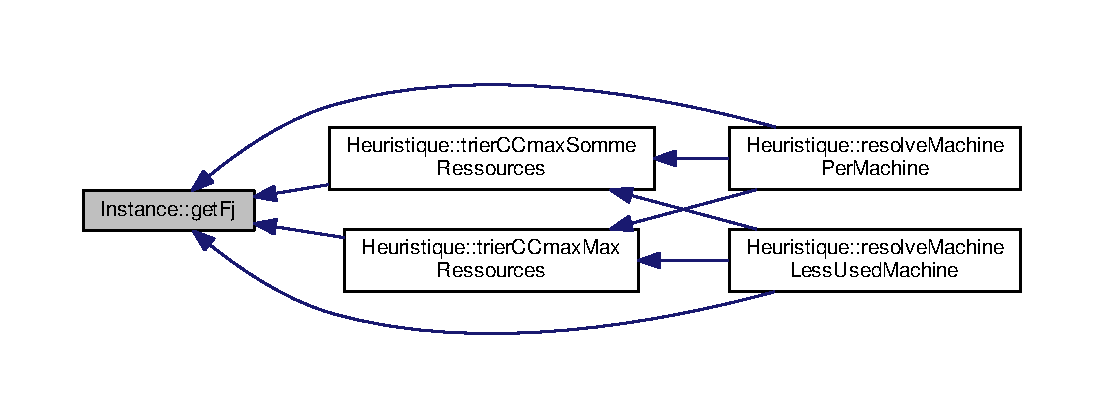
\includegraphics[width=350pt]{classInstance_af7b70cbd8670e4eb213fbd2b81eca6f0_icgraph}
\end{center}
\end{figure}
\mbox{\Hypertarget{classInstance_a8bf10528309a62149cc188dd2b80f0b7}\label{classInstance_a8bf10528309a62149cc188dd2b80f0b7}} 
\index{Instance@{Instance}!get\+Horizon\+Max@{get\+Horizon\+Max}}
\index{get\+Horizon\+Max@{get\+Horizon\+Max}!Instance@{Instance}}
\subsubsection{\texorpdfstring{get\+Horizon\+Max()}{getHorizonMax()}}
{\footnotesize\ttfamily unsigned int Instance\+::get\+Horizon\+Max (\begin{DoxyParamCaption}{ }\end{DoxyParamCaption}) const}



Permet d\textquotesingle{}obtenir l\textquotesingle{}horizon maximale de planification de l\textquotesingle{}instance. 

\begin{DoxyReturn}{Returns}
unsigned int L\textquotesingle{}horizon maximale de planification de l\textquotesingle{}instance 
\end{DoxyReturn}
\mbox{\Hypertarget{classInstance_a1ed694b05c888cdb177ddf4c92a482d9}\label{classInstance_a1ed694b05c888cdb177ddf4c92a482d9}} 
\index{Instance@{Instance}!get\+Nbr\+Jobs@{get\+Nbr\+Jobs}}
\index{get\+Nbr\+Jobs@{get\+Nbr\+Jobs}!Instance@{Instance}}
\subsubsection{\texorpdfstring{get\+Nbr\+Jobs()}{getNbrJobs()}}
{\footnotesize\ttfamily unsigned int Instance\+::get\+Nbr\+Jobs (\begin{DoxyParamCaption}{ }\end{DoxyParamCaption}) const}



Permet d\textquotesingle{}obtenir le nombre de jobs de l\textquotesingle{}instance. 

\begin{DoxyReturn}{Returns}
unsigned int Le nombre de jobs 
\end{DoxyReturn}
Here is the caller graph for this function\+:\nopagebreak
\begin{figure}[H]
\begin{center}
\leavevmode
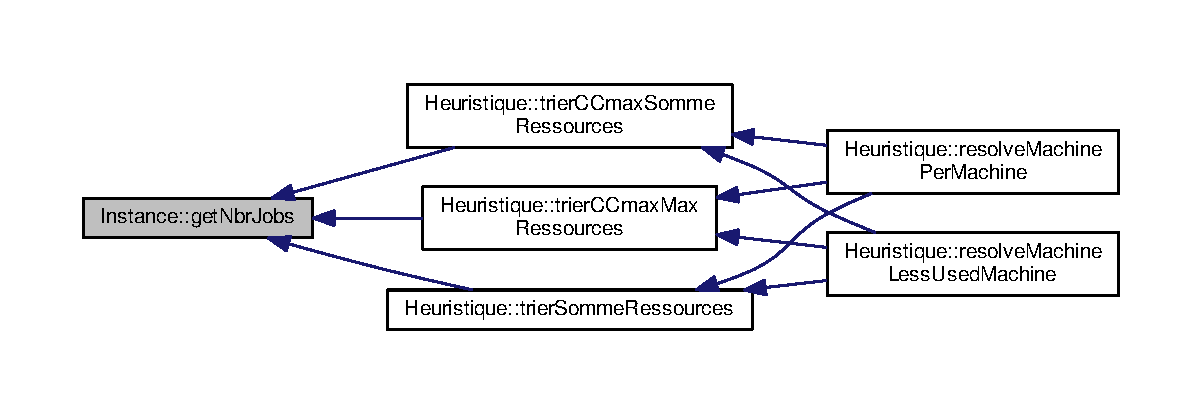
\includegraphics[width=350pt]{classInstance_a1ed694b05c888cdb177ddf4c92a482d9_icgraph}
\end{center}
\end{figure}
\mbox{\Hypertarget{classInstance_a2f985b9a7ce18fd8739ec589d9016003}\label{classInstance_a2f985b9a7ce18fd8739ec589d9016003}} 
\index{Instance@{Instance}!get\+Nbr\+Machines@{get\+Nbr\+Machines}}
\index{get\+Nbr\+Machines@{get\+Nbr\+Machines}!Instance@{Instance}}
\subsubsection{\texorpdfstring{get\+Nbr\+Machines()}{getNbrMachines()}}
{\footnotesize\ttfamily unsigned int Instance\+::get\+Nbr\+Machines (\begin{DoxyParamCaption}{ }\end{DoxyParamCaption}) const}



Permet d\textquotesingle{}obtenir le nombre de machines de l\textquotesingle{}instance. 

\begin{DoxyReturn}{Returns}
unsigned int Le nombre de machines 
\end{DoxyReturn}
Here is the caller graph for this function\+:\nopagebreak
\begin{figure}[H]
\begin{center}
\leavevmode
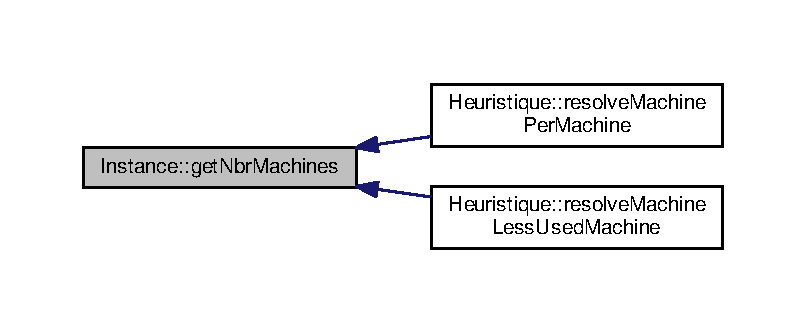
\includegraphics[width=350pt]{classInstance_a2f985b9a7ce18fd8739ec589d9016003_icgraph}
\end{center}
\end{figure}
\mbox{\Hypertarget{classInstance_a79b49dcc3d590b823e41d8a223ecf25d}\label{classInstance_a79b49dcc3d590b823e41d8a223ecf25d}} 
\index{Instance@{Instance}!get\+Nbr\+Ressources@{get\+Nbr\+Ressources}}
\index{get\+Nbr\+Ressources@{get\+Nbr\+Ressources}!Instance@{Instance}}
\subsubsection{\texorpdfstring{get\+Nbr\+Ressources()}{getNbrRessources()}}
{\footnotesize\ttfamily unsigned int Instance\+::get\+Nbr\+Ressources (\begin{DoxyParamCaption}{ }\end{DoxyParamCaption}) const}



Permet d\textquotesingle{}obtenir le nombre de ressources de l\textquotesingle{}instance. 

\begin{DoxyReturn}{Returns}
unsigned int Le nombre de ressources 
\end{DoxyReturn}
Here is the caller graph for this function\+:
\nopagebreak
\begin{figure}[H]
\begin{center}
\leavevmode
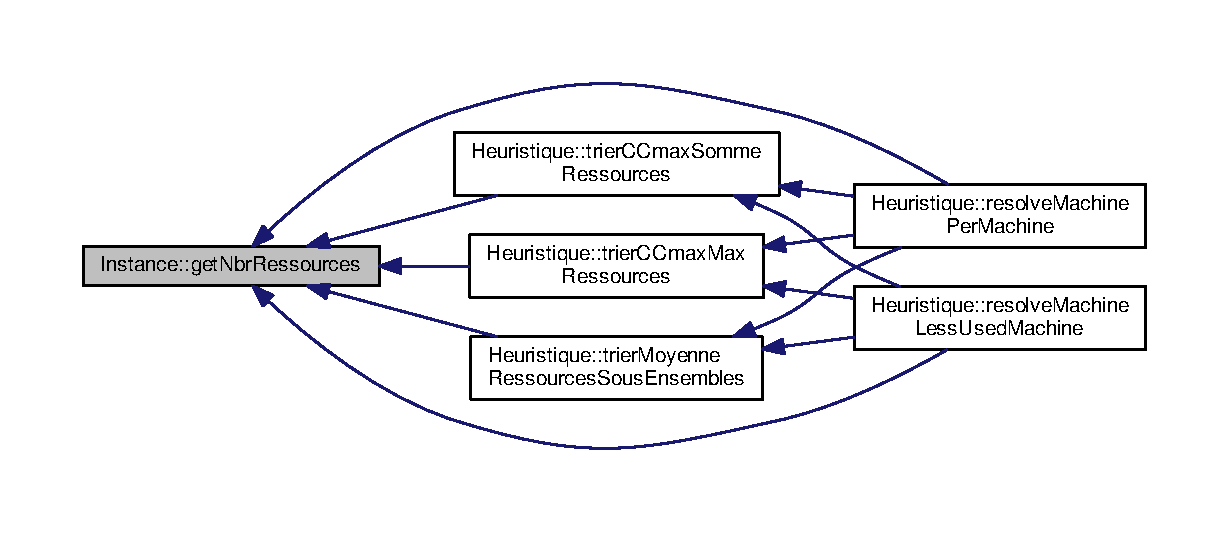
\includegraphics[width=350pt]{classInstance_a79b49dcc3d590b823e41d8a223ecf25d_icgraph}
\end{center}
\end{figure}
\mbox{\Hypertarget{classInstance_ab998bc8d9a8b03c8f6279573779217cc}\label{classInstance_ab998bc8d9a8b03c8f6279573779217cc}} 
\index{Instance@{Instance}!get\+Sj@{get\+Sj}}
\index{get\+Sj@{get\+Sj}!Instance@{Instance}}
\subsubsection{\texorpdfstring{get\+Sj()}{getSj()}}
{\footnotesize\ttfamily vector$<$ unsigned int $>$ Instance\+::get\+Sj (\begin{DoxyParamCaption}{ }\end{DoxyParamCaption}) const}



Permet d\textquotesingle{}obtenir le tableau des instants de départ de l\textquotesingle{}ensemble des jobs. 

\begin{DoxyReturn}{Returns}
vector$<$unsigned int$>$ Le tableau des instants de départ de l\textquotesingle{}ensemble des jobs 
\end{DoxyReturn}
Here is the caller graph for this function\+:
\nopagebreak
\begin{figure}[H]
\begin{center}
\leavevmode
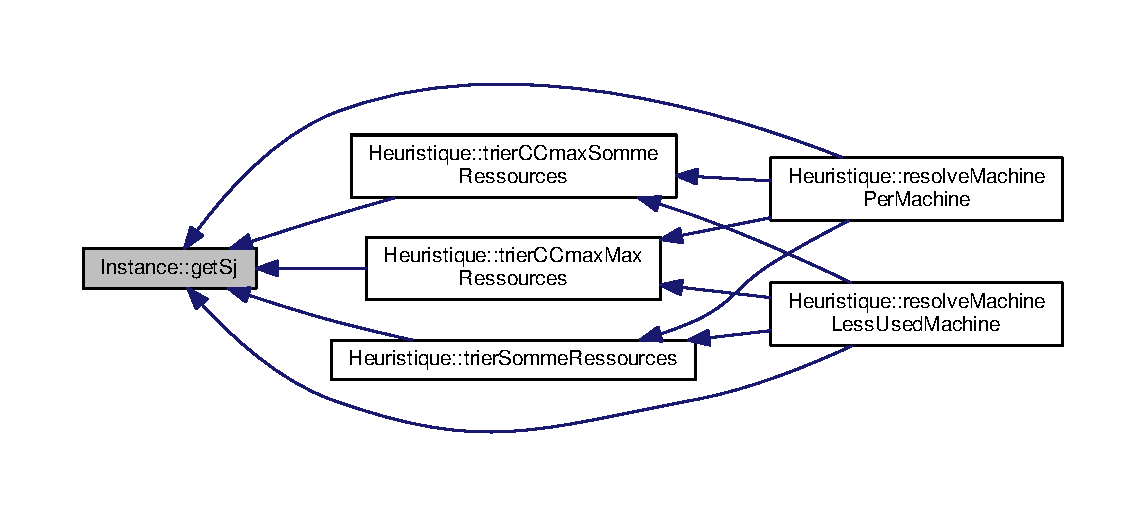
\includegraphics[width=350pt]{classInstance_ab998bc8d9a8b03c8f6279573779217cc_icgraph}
\end{center}
\end{figure}
\mbox{\Hypertarget{classInstance_a2011ff3253fcb1d2d354c3c34a14a6fb}\label{classInstance_a2011ff3253fcb1d2d354c3c34a14a6fb}} 
\index{Instance@{Instance}!get\+Sous\+Ensembles\+Maximaux@{get\+Sous\+Ensembles\+Maximaux}}
\index{get\+Sous\+Ensembles\+Maximaux@{get\+Sous\+Ensembles\+Maximaux}!Instance@{Instance}}
\subsubsection{\texorpdfstring{get\+Sous\+Ensembles\+Maximaux()}{getSousEnsemblesMaximaux()}}
{\footnotesize\ttfamily map$<$ unsigned int, vector$<$ unsigned int $>$ $>$ Instance\+::get\+Sous\+Ensembles\+Maximaux (\begin{DoxyParamCaption}{ }\end{DoxyParamCaption})}



Retourne les sous-\/ensembles maximaux de jobs de l\textquotesingle{}instance (jobs se chevauchant) 

\begin{DoxyReturn}{Returns}
map$<$unsigned int, vector$<$unsigned int$>$ $>$ Les sous-\/ensembles maximaux de jobs de l\textquotesingle{}instance 
\end{DoxyReturn}
Here is the caller graph for this function\+:
\nopagebreak
\begin{figure}[H]
\begin{center}
\leavevmode
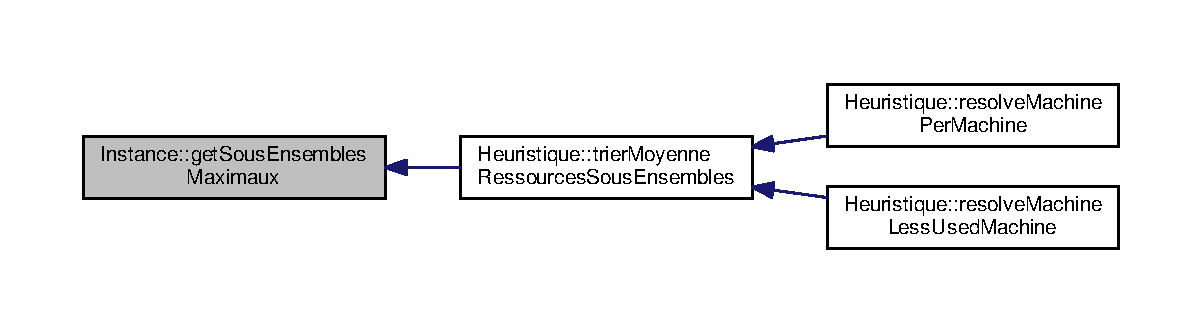
\includegraphics[width=350pt]{classInstance_a2011ff3253fcb1d2d354c3c34a14a6fb_icgraph}
\end{center}
\end{figure}
\mbox{\Hypertarget{classInstance_ad4124bd2f1edb83a46ef94cfe07eafc8}\label{classInstance_ad4124bd2f1edb83a46ef94cfe07eafc8}} 
\index{Instance@{Instance}!get\+Tableau\+Ressources\+Jobs@{get\+Tableau\+Ressources\+Jobs}}
\index{get\+Tableau\+Ressources\+Jobs@{get\+Tableau\+Ressources\+Jobs}!Instance@{Instance}}
\subsubsection{\texorpdfstring{get\+Tableau\+Ressources\+Jobs()}{getTableauRessourcesJobs()}}
{\footnotesize\ttfamily vector$<$ vector$<$ unsigned int $>$ $>$ Instance\+::get\+Tableau\+Ressources\+Jobs (\begin{DoxyParamCaption}{ }\end{DoxyParamCaption}) const}



Permet d\textquotesingle{}obtenir le tableau des capacités en ressource pour l\textquotesingle{}ensemble des jobs. 

\begin{DoxyReturn}{Returns}
vector$<$vector$<$unsigned int$>$$>$ Le tableau des capacités en ressource pour l\textquotesingle{}ensemble des jobs 
\end{DoxyReturn}
Here is the caller graph for this function\+:
\nopagebreak
\begin{figure}[H]
\begin{center}
\leavevmode
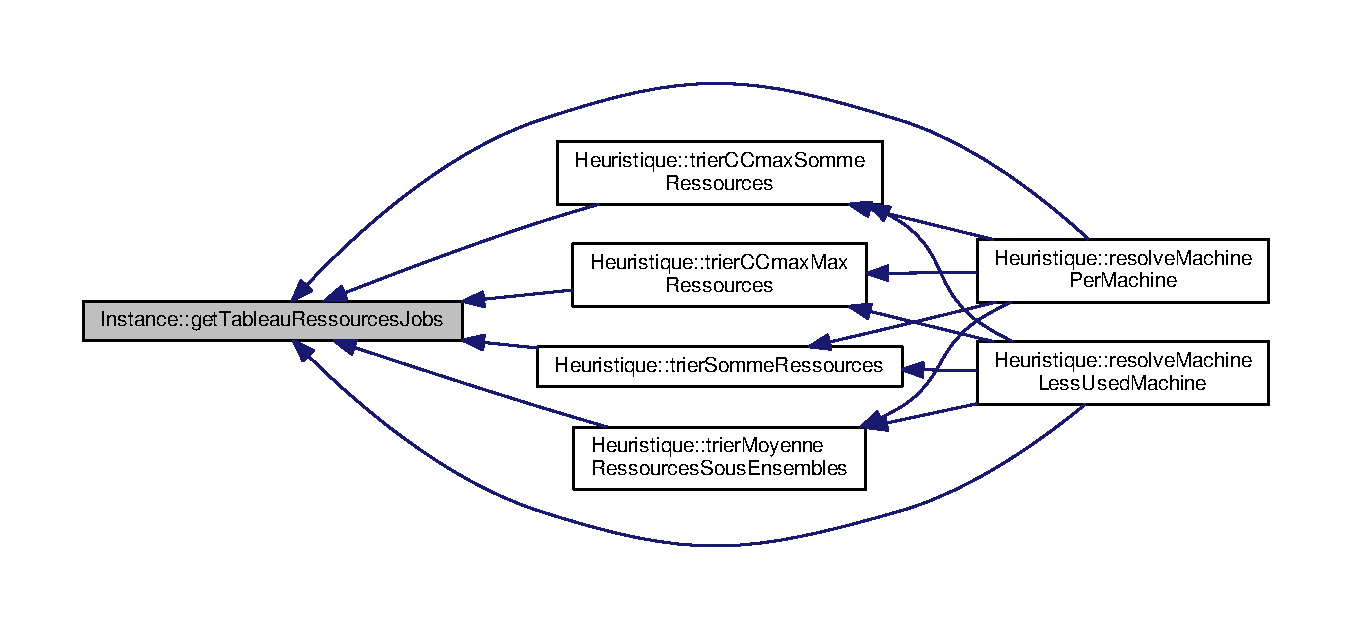
\includegraphics[width=350pt]{classInstance_ad4124bd2f1edb83a46ef94cfe07eafc8_icgraph}
\end{center}
\end{figure}
\mbox{\Hypertarget{classInstance_a36e8de8c42d48f16f14f37622dbd3eb1}\label{classInstance_a36e8de8c42d48f16f14f37622dbd3eb1}} 
\index{Instance@{Instance}!sauvegarder\+Instance@{sauvegarder\+Instance}}
\index{sauvegarder\+Instance@{sauvegarder\+Instance}!Instance@{Instance}}
\subsubsection{\texorpdfstring{sauvegarder\+Instance()}{sauvegarderInstance()}}
{\footnotesize\ttfamily void Instance\+::sauvegarder\+Instance (\begin{DoxyParamCaption}\item[{unsigned int}]{nbr\+Instance,  }\item[{unsigned int}]{nbr\+Jobs,  }\item[{unsigned int}]{nbr\+Ressources,  }\item[{unsigned int}]{nbr\+Machines,  }\item[{unsigned int}]{horizon\+Planification }\end{DoxyParamCaption})}



Permet de sauvegarder des instances avec des paramètres particuliers. 


\begin{DoxyParams}{Parameters}
{\em nbr\+Instance} & Le nombre d\textquotesingle{}instance à générer \\
\hline
{\em nbr\+Jobs} & Le nombre de jobs par instance \\
\hline
{\em nbr\+Ressources} & Le nombre de ressources par instance \\
\hline
{\em nbr\+Machines} & Le nombre de machines par instance \\
\hline
{\em horizon\+Planification} & L\textquotesingle{}horizon de planification maximal de chaque instance \\
\hline
\end{DoxyParams}
Here is the caller graph for this function\+:
\nopagebreak
\begin{figure}[H]
\begin{center}
\leavevmode
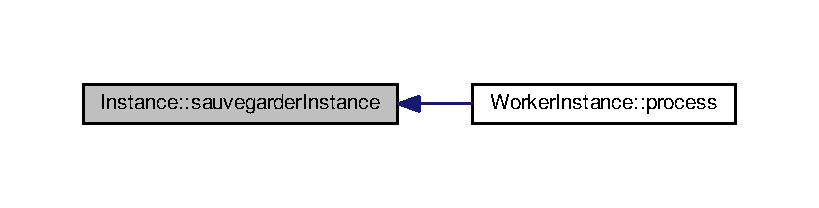
\includegraphics[width=350pt]{classInstance_a36e8de8c42d48f16f14f37622dbd3eb1_icgraph}
\end{center}
\end{figure}
\mbox{\Hypertarget{classInstance_a527d6a6623e0257f4512a96285a960a5}\label{classInstance_a527d6a6623e0257f4512a96285a960a5}} 
\index{Instance@{Instance}!set\+Cap\+Ressources@{set\+Cap\+Ressources}}
\index{set\+Cap\+Ressources@{set\+Cap\+Ressources}!Instance@{Instance}}
\subsubsection{\texorpdfstring{set\+Cap\+Ressources()}{setCapRessources()}}
{\footnotesize\ttfamily void Instance\+::set\+Cap\+Ressources (\begin{DoxyParamCaption}\item[{const vector$<$ vector$<$ unsigned int $>$$>$ \&}]{value }\end{DoxyParamCaption})}



Setter du tableau des capacités en ressource pour l\textquotesingle{}ensemble des machines. 


\begin{DoxyParams}{Parameters}
{\em value} & Le tableau des capacités en ressource pour l\textquotesingle{}ensemble des machines souhaité \\
\hline
\end{DoxyParams}
\mbox{\Hypertarget{classInstance_a263461a7a8c44c9e7080620a30cc8fcf}\label{classInstance_a263461a7a8c44c9e7080620a30cc8fcf}} 
\index{Instance@{Instance}!set\+Fichier\+Instance@{set\+Fichier\+Instance}}
\index{set\+Fichier\+Instance@{set\+Fichier\+Instance}!Instance@{Instance}}
\subsubsection{\texorpdfstring{set\+Fichier\+Instance()}{setFichierInstance()}}
{\footnotesize\ttfamily void Instance\+::set\+Fichier\+Instance (\begin{DoxyParamCaption}\item[{const Q\+String \&}]{value }\end{DoxyParamCaption})}



Setter du chemin vers le fichier d\textquotesingle{}instance. 


\begin{DoxyParams}{Parameters}
{\em value} & Le chemin vers le fichier d\textquotesingle{}instance que l\textquotesingle{}on souhaite \\
\hline
\end{DoxyParams}
\mbox{\Hypertarget{classInstance_a544764ab0dcb42e795c5bfee4a0681cf}\label{classInstance_a544764ab0dcb42e795c5bfee4a0681cf}} 
\index{Instance@{Instance}!set\+Fj@{set\+Fj}}
\index{set\+Fj@{set\+Fj}!Instance@{Instance}}
\subsubsection{\texorpdfstring{set\+Fj()}{setFj()}}
{\footnotesize\ttfamily void Instance\+::set\+Fj (\begin{DoxyParamCaption}\item[{const vector$<$ unsigned int $>$ \&}]{value }\end{DoxyParamCaption})}



Setter du tableau des instants de fin de l\textquotesingle{}ensemble des jobs. 


\begin{DoxyParams}{Parameters}
{\em value} & Le tableau des instants de fin de l\textquotesingle{}ensemble des jobs souhaité \\
\hline
\end{DoxyParams}
\mbox{\Hypertarget{classInstance_aca68cfedc71eb3b2e7051ef99412e965}\label{classInstance_aca68cfedc71eb3b2e7051ef99412e965}} 
\index{Instance@{Instance}!set\+Horizon\+Max@{set\+Horizon\+Max}}
\index{set\+Horizon\+Max@{set\+Horizon\+Max}!Instance@{Instance}}
\subsubsection{\texorpdfstring{set\+Horizon\+Max()}{setHorizonMax()}}
{\footnotesize\ttfamily void Instance\+::set\+Horizon\+Max (\begin{DoxyParamCaption}\item[{unsigned int}]{value }\end{DoxyParamCaption})}



Setter de l\textquotesingle{}horizon maximale de planification de l\textquotesingle{}instance. 


\begin{DoxyParams}{Parameters}
{\em value} & L\textquotesingle{}horizon maximale de planification de l\textquotesingle{}instance souhaitée \\
\hline
\end{DoxyParams}
\mbox{\Hypertarget{classInstance_ade6c7b12ee34960cebb060d669ec8f06}\label{classInstance_ade6c7b12ee34960cebb060d669ec8f06}} 
\index{Instance@{Instance}!set\+Nbr\+Jobs@{set\+Nbr\+Jobs}}
\index{set\+Nbr\+Jobs@{set\+Nbr\+Jobs}!Instance@{Instance}}
\subsubsection{\texorpdfstring{set\+Nbr\+Jobs()}{setNbrJobs()}}
{\footnotesize\ttfamily void Instance\+::set\+Nbr\+Jobs (\begin{DoxyParamCaption}\item[{unsigned int}]{value }\end{DoxyParamCaption})}



Setter du nombre de jobs de l\textquotesingle{}instance. 


\begin{DoxyParams}{Parameters}
{\em value} & Le nombre de jobs souhaité de l\textquotesingle{}instance \\
\hline
\end{DoxyParams}
\mbox{\Hypertarget{classInstance_a7087e8d1d2a5a4d275472dc908a06381}\label{classInstance_a7087e8d1d2a5a4d275472dc908a06381}} 
\index{Instance@{Instance}!set\+Nbr\+Machines@{set\+Nbr\+Machines}}
\index{set\+Nbr\+Machines@{set\+Nbr\+Machines}!Instance@{Instance}}
\subsubsection{\texorpdfstring{set\+Nbr\+Machines()}{setNbrMachines()}}
{\footnotesize\ttfamily void Instance\+::set\+Nbr\+Machines (\begin{DoxyParamCaption}\item[{unsigned int}]{value }\end{DoxyParamCaption})}



Setter du nombre de machines de l\textquotesingle{}instance. 


\begin{DoxyParams}{Parameters}
{\em value} & Le nombre de machines souhaité de l\textquotesingle{}instance \\
\hline
\end{DoxyParams}
\mbox{\Hypertarget{classInstance_aefc2e4c0a18ad899f99cad856a749358}\label{classInstance_aefc2e4c0a18ad899f99cad856a749358}} 
\index{Instance@{Instance}!set\+Nbr\+Ressources@{set\+Nbr\+Ressources}}
\index{set\+Nbr\+Ressources@{set\+Nbr\+Ressources}!Instance@{Instance}}
\subsubsection{\texorpdfstring{set\+Nbr\+Ressources()}{setNbrRessources()}}
{\footnotesize\ttfamily void Instance\+::set\+Nbr\+Ressources (\begin{DoxyParamCaption}\item[{unsigned int}]{value }\end{DoxyParamCaption})}



Setter du nombre de ressources de l\textquotesingle{}instance. 


\begin{DoxyParams}{Parameters}
{\em value} & Le nombre de ressources souhaité de l\textquotesingle{}instance \\
\hline
\end{DoxyParams}
\mbox{\Hypertarget{classInstance_af695a8a91368f2484ee7367b14144742}\label{classInstance_af695a8a91368f2484ee7367b14144742}} 
\index{Instance@{Instance}!set\+Sj@{set\+Sj}}
\index{set\+Sj@{set\+Sj}!Instance@{Instance}}
\subsubsection{\texorpdfstring{set\+Sj()}{setSj()}}
{\footnotesize\ttfamily void Instance\+::set\+Sj (\begin{DoxyParamCaption}\item[{const vector$<$ unsigned int $>$ \&}]{value }\end{DoxyParamCaption})}



Setter du tableau des instants de départ de l\textquotesingle{}ensemble des jobs. 


\begin{DoxyParams}{Parameters}
{\em value} & Le tableau des instants de départ de l\textquotesingle{}ensemble des jobs souhaité \\
\hline
\end{DoxyParams}
\mbox{\Hypertarget{classInstance_a702ba79351487440788af8d662f1266c}\label{classInstance_a702ba79351487440788af8d662f1266c}} 
\index{Instance@{Instance}!set\+Tableau\+Ressources\+Jobs@{set\+Tableau\+Ressources\+Jobs}}
\index{set\+Tableau\+Ressources\+Jobs@{set\+Tableau\+Ressources\+Jobs}!Instance@{Instance}}
\subsubsection{\texorpdfstring{set\+Tableau\+Ressources\+Jobs()}{setTableauRessourcesJobs()}}
{\footnotesize\ttfamily void Instance\+::set\+Tableau\+Ressources\+Jobs (\begin{DoxyParamCaption}\item[{const vector$<$ vector$<$ unsigned int $>$ $>$ \&}]{value }\end{DoxyParamCaption})}



Setter du tableau des capacités en ressource pour l\textquotesingle{}ensemble des jobs. 


\begin{DoxyParams}{Parameters}
{\em value} & Le tableau des capacités en ressource pour l\textquotesingle{}ensemble des jobs souhaité \\
\hline
\end{DoxyParams}


The documentation for this class was generated from the following files\+:\begin{DoxyCompactItemize}
\item 
P\+R\+D\+Ordonancement/\hyperlink{instance_8h}{instance.\+h}\item 
P\+R\+D\+Ordonancement/\hyperlink{instance_8cpp}{instance.\+cpp}\end{DoxyCompactItemize}

\hypertarget{classMethodeExacte}{}\section{Methode\+Exacte Class Reference}
\label{classMethodeExacte}\index{Methode\+Exacte@{Methode\+Exacte}}


Classe \hyperlink{classMethodeExacte}{Methode\+Exacte} permetant de résoudre des instances à l\textquotesingle{}aide de méthodes exactes.  




{\ttfamily \#include $<$methodeexacte.\+h$>$}

\subsection*{Public Member Functions}
\begin{DoxyCompactItemize}
\item 
\hyperlink{classMethodeExacte_a82cea9720ff44a85f2c991f601ffd53b}{Methode\+Exacte} (string fichier\+Instance, map$<$ unsigned int, unsigned int $>$ pourcentages\+Par\+Agent)
\begin{DoxyCompactList}\small\item\em Constructeur de la classe \hyperlink{classMethodeExacte}{Methode\+Exacte}. \end{DoxyCompactList}\item 
unsigned int \hyperlink{classMethodeExacte_a91443b3ea749912772b40b5b5c40379e}{resolution\+Plne\+Mip1} (string fichier\+Resultat)
\begin{DoxyCompactList}\small\item\em Methode de résolution exacte indéxée temps. \end{DoxyCompactList}\item 
unsigned int \hyperlink{classMethodeExacte_a3163e487cc9e99ee7667d1dd146edb4b}{resolution\+Plne\+Mip2} (string fichier\+Resultat)
\begin{DoxyCompactList}\small\item\em Methode de résolution exacte indéxée jobs. \end{DoxyCompactList}\item 
unsigned int \hyperlink{classMethodeExacte_a3b3d9ad4a6d21f6e3be43212eb706054}{resolution\+Plne\+Mip1\+Multi\+Agent} (string fichier\+Resultat)
\begin{DoxyCompactList}\small\item\em Methode de résolution exacte indéxée temps pour un cas multi agent. \end{DoxyCompactList}\item 
unsigned int \hyperlink{classMethodeExacte_af5ed64d8d21ead081e02c3ac97192859}{resolution\+Plne\+Mip2\+Multi\+Agent} (string fichier\+Resultat)
\begin{DoxyCompactList}\small\item\em Methode de résolution exacte indéxée jobs pour un cas multi agent. \end{DoxyCompactList}\item 
\hyperlink{classInstance}{Instance} \hyperlink{classMethodeExacte_a6c8b291d40a0e9c3df51ea367d43189c}{get\+Instance} () const
\item 
void \hyperlink{classMethodeExacte_ae4a99972ce73ff50611a8842506723f9}{set\+Instance} (const \hyperlink{classInstance}{Instance} \&value)
\end{DoxyCompactItemize}


\subsection{Detailed Description}
Classe \hyperlink{classMethodeExacte}{Methode\+Exacte} permetant de résoudre des instances à l\textquotesingle{}aide de méthodes exactes. 

\subsection{Constructor \& Destructor Documentation}
\mbox{\Hypertarget{classMethodeExacte_a82cea9720ff44a85f2c991f601ffd53b}\label{classMethodeExacte_a82cea9720ff44a85f2c991f601ffd53b}} 
\index{Methode\+Exacte@{Methode\+Exacte}!Methode\+Exacte@{Methode\+Exacte}}
\index{Methode\+Exacte@{Methode\+Exacte}!Methode\+Exacte@{Methode\+Exacte}}
\subsubsection{\texorpdfstring{Methode\+Exacte()}{MethodeExacte()}}
{\footnotesize\ttfamily Methode\+Exacte\+::\+Methode\+Exacte (\begin{DoxyParamCaption}\item[{string}]{fichier\+Instance,  }\item[{map$<$ unsigned int, unsigned int $>$}]{pourcentages\+Par\+Agent }\end{DoxyParamCaption})}



Constructeur de la classe \hyperlink{classMethodeExacte}{Methode\+Exacte}. 


\begin{DoxyParams}{Parameters}
{\em fichier\+Instance} & Le chemin vers le fichier d\textquotesingle{}instance \\
\hline
\end{DoxyParams}


\subsection{Member Function Documentation}
\mbox{\Hypertarget{classMethodeExacte_a6c8b291d40a0e9c3df51ea367d43189c}\label{classMethodeExacte_a6c8b291d40a0e9c3df51ea367d43189c}} 
\index{Methode\+Exacte@{Methode\+Exacte}!get\+Instance@{get\+Instance}}
\index{get\+Instance@{get\+Instance}!Methode\+Exacte@{Methode\+Exacte}}
\subsubsection{\texorpdfstring{get\+Instance()}{getInstance()}}
{\footnotesize\ttfamily \hyperlink{classInstance}{Instance} Methode\+Exacte\+::get\+Instance (\begin{DoxyParamCaption}{ }\end{DoxyParamCaption}) const}

\mbox{\Hypertarget{classMethodeExacte_a91443b3ea749912772b40b5b5c40379e}\label{classMethodeExacte_a91443b3ea749912772b40b5b5c40379e}} 
\index{Methode\+Exacte@{Methode\+Exacte}!resolution\+Plne\+Mip1@{resolution\+Plne\+Mip1}}
\index{resolution\+Plne\+Mip1@{resolution\+Plne\+Mip1}!Methode\+Exacte@{Methode\+Exacte}}
\subsubsection{\texorpdfstring{resolution\+Plne\+Mip1()}{resolutionPlneMip1()}}
{\footnotesize\ttfamily unsigned int Methode\+Exacte\+::resolution\+Plne\+Mip1 (\begin{DoxyParamCaption}\item[{string}]{fichier\+Resultat }\end{DoxyParamCaption})}



Methode de résolution exacte indéxée temps. 


\begin{DoxyParams}{Parameters}
{\em fichier\+Resultat} & Le fichier où seront stockés les résulats \\
\hline
\end{DoxyParams}
\begin{DoxyReturn}{Returns}
unsigned int Le nombre de jobs ordonnancés 
\end{DoxyReturn}
Here is the caller graph for this function\+:\nopagebreak
\begin{figure}[H]
\begin{center}
\leavevmode
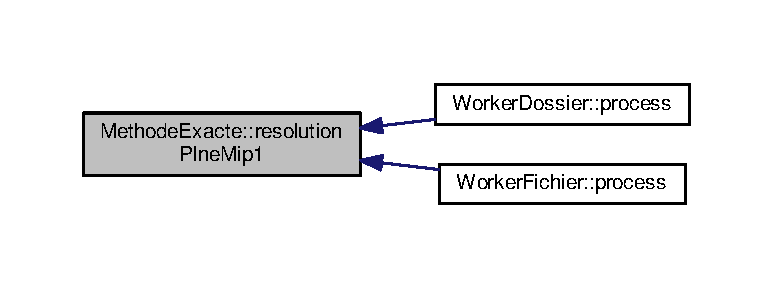
\includegraphics[width=350pt]{classMethodeExacte_a91443b3ea749912772b40b5b5c40379e_icgraph}
\end{center}
\end{figure}
\mbox{\Hypertarget{classMethodeExacte_a3b3d9ad4a6d21f6e3be43212eb706054}\label{classMethodeExacte_a3b3d9ad4a6d21f6e3be43212eb706054}} 
\index{Methode\+Exacte@{Methode\+Exacte}!resolution\+Plne\+Mip1\+Multi\+Agent@{resolution\+Plne\+Mip1\+Multi\+Agent}}
\index{resolution\+Plne\+Mip1\+Multi\+Agent@{resolution\+Plne\+Mip1\+Multi\+Agent}!Methode\+Exacte@{Methode\+Exacte}}
\subsubsection{\texorpdfstring{resolution\+Plne\+Mip1\+Multi\+Agent()}{resolutionPlneMip1MultiAgent()}}
{\footnotesize\ttfamily unsigned int Methode\+Exacte\+::resolution\+Plne\+Mip1\+Multi\+Agent (\begin{DoxyParamCaption}\item[{string}]{fichier\+Resultat }\end{DoxyParamCaption})}



Methode de résolution exacte indéxée temps pour un cas multi agent. 


\begin{DoxyParams}{Parameters}
{\em fichier\+Resultat} & Le fichier où seront stockés les résulats \\
\hline
\end{DoxyParams}
\begin{DoxyReturn}{Returns}
unsigned int Le nombre de jobs ordonnancés 
\end{DoxyReturn}
Here is the caller graph for this function\+:\nopagebreak
\begin{figure}[H]
\begin{center}
\leavevmode
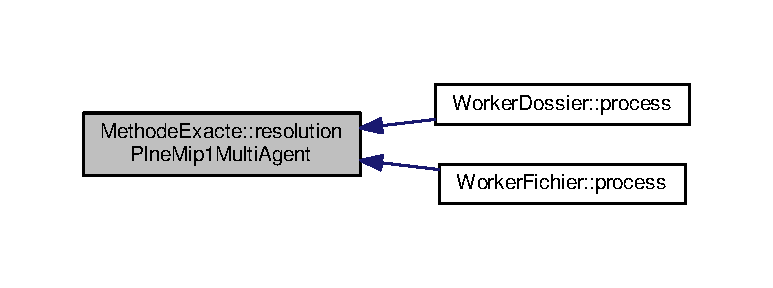
\includegraphics[width=350pt]{classMethodeExacte_a3b3d9ad4a6d21f6e3be43212eb706054_icgraph}
\end{center}
\end{figure}
\mbox{\Hypertarget{classMethodeExacte_a3163e487cc9e99ee7667d1dd146edb4b}\label{classMethodeExacte_a3163e487cc9e99ee7667d1dd146edb4b}} 
\index{Methode\+Exacte@{Methode\+Exacte}!resolution\+Plne\+Mip2@{resolution\+Plne\+Mip2}}
\index{resolution\+Plne\+Mip2@{resolution\+Plne\+Mip2}!Methode\+Exacte@{Methode\+Exacte}}
\subsubsection{\texorpdfstring{resolution\+Plne\+Mip2()}{resolutionPlneMip2()}}
{\footnotesize\ttfamily unsigned int Methode\+Exacte\+::resolution\+Plne\+Mip2 (\begin{DoxyParamCaption}\item[{string}]{fichier\+Resultat }\end{DoxyParamCaption})}



Methode de résolution exacte indéxée jobs. 


\begin{DoxyParams}{Parameters}
{\em fichier\+Resultat} & Le fichier où seront stockés les résulats \\
\hline
\end{DoxyParams}
\begin{DoxyReturn}{Returns}
unsigned int Le nombre de jobs ordonnancés 
\end{DoxyReturn}
Here is the caller graph for this function\+:\nopagebreak
\begin{figure}[H]
\begin{center}
\leavevmode
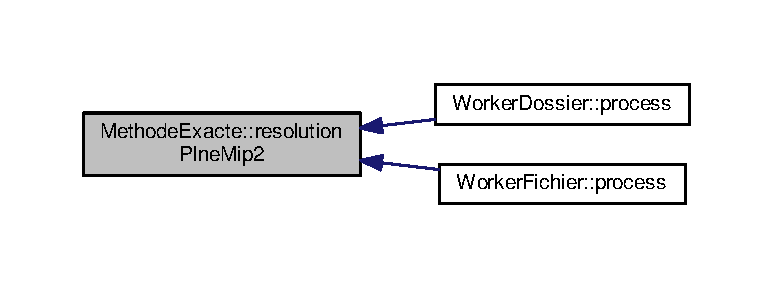
\includegraphics[width=350pt]{classMethodeExacte_a3163e487cc9e99ee7667d1dd146edb4b_icgraph}
\end{center}
\end{figure}
\mbox{\Hypertarget{classMethodeExacte_af5ed64d8d21ead081e02c3ac97192859}\label{classMethodeExacte_af5ed64d8d21ead081e02c3ac97192859}} 
\index{Methode\+Exacte@{Methode\+Exacte}!resolution\+Plne\+Mip2\+Multi\+Agent@{resolution\+Plne\+Mip2\+Multi\+Agent}}
\index{resolution\+Plne\+Mip2\+Multi\+Agent@{resolution\+Plne\+Mip2\+Multi\+Agent}!Methode\+Exacte@{Methode\+Exacte}}
\subsubsection{\texorpdfstring{resolution\+Plne\+Mip2\+Multi\+Agent()}{resolutionPlneMip2MultiAgent()}}
{\footnotesize\ttfamily unsigned int Methode\+Exacte\+::resolution\+Plne\+Mip2\+Multi\+Agent (\begin{DoxyParamCaption}\item[{string}]{fichier\+Resultat }\end{DoxyParamCaption})}



Methode de résolution exacte indéxée jobs pour un cas multi agent. 


\begin{DoxyParams}{Parameters}
{\em fichier\+Resultat} & Le fichier où seront stockés les résulats \\
\hline
\end{DoxyParams}
\begin{DoxyReturn}{Returns}
unsigned int Le nombre de jobs ordonnancés 
\end{DoxyReturn}
Here is the caller graph for this function\+:\nopagebreak
\begin{figure}[H]
\begin{center}
\leavevmode
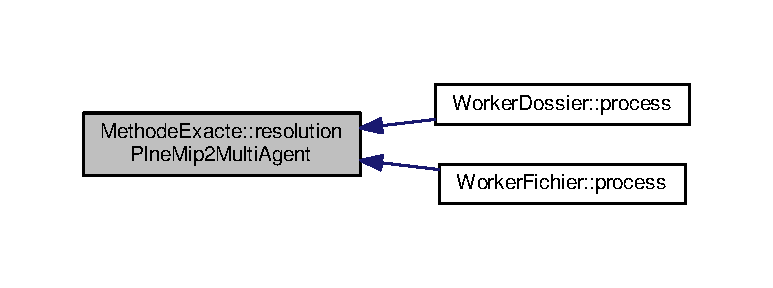
\includegraphics[width=350pt]{classMethodeExacte_af5ed64d8d21ead081e02c3ac97192859_icgraph}
\end{center}
\end{figure}
\mbox{\Hypertarget{classMethodeExacte_ae4a99972ce73ff50611a8842506723f9}\label{classMethodeExacte_ae4a99972ce73ff50611a8842506723f9}} 
\index{Methode\+Exacte@{Methode\+Exacte}!set\+Instance@{set\+Instance}}
\index{set\+Instance@{set\+Instance}!Methode\+Exacte@{Methode\+Exacte}}
\subsubsection{\texorpdfstring{set\+Instance()}{setInstance()}}
{\footnotesize\ttfamily void Methode\+Exacte\+::set\+Instance (\begin{DoxyParamCaption}\item[{const \hyperlink{classInstance}{Instance} \&}]{value }\end{DoxyParamCaption})}



The documentation for this class was generated from the following files\+:\begin{DoxyCompactItemize}
\item 
P\+R\+D\+Ordonancement/\hyperlink{methodeexacte_8h}{methodeexacte.\+h}\item 
P\+R\+D\+Ordonancement/\hyperlink{methodeexacte_01_07copy_011_08_8cpp}{methodeexacte (copy 1).\+cpp}\item 
P\+R\+D\+Ordonancement/\hyperlink{methodeexacte_8cpp}{methodeexacte.\+cpp}\end{DoxyCompactItemize}

\hypertarget{classResolutionInstance}{}\section{Resolution\+Instance Class Reference}
\label{classResolutionInstance}\index{Resolution\+Instance@{Resolution\+Instance}}


Fenêtre \hyperlink{classResolutionInstance}{Resolution\+Instance}.  




{\ttfamily \#include $<$resolutioninstance.\+h$>$}



Inheritance diagram for Resolution\+Instance\+:\nopagebreak
\begin{figure}[H]
\begin{center}
\leavevmode
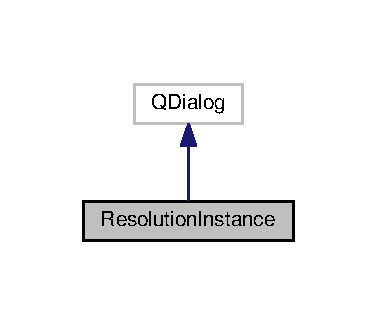
\includegraphics[width=181pt]{classResolutionInstance__inherit__graph}
\end{center}
\end{figure}


Collaboration diagram for Resolution\+Instance\+:\nopagebreak
\begin{figure}[H]
\begin{center}
\leavevmode
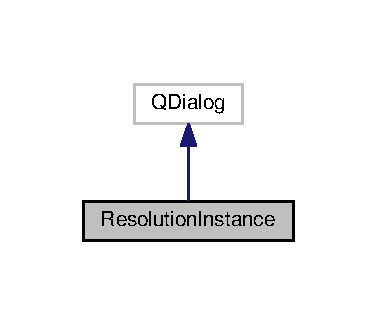
\includegraphics[width=181pt]{classResolutionInstance__coll__graph}
\end{center}
\end{figure}
\subsection*{Public Member Functions}
\begin{DoxyCompactItemize}
\item 
\hyperlink{classResolutionInstance_a90e1ee7d8245bed88624a159b00cb6a7}{Resolution\+Instance} (Q\+Widget $\ast$parent=0)
\begin{DoxyCompactList}\small\item\em Constructeur de la classe \hyperlink{classResolutionInstance}{Resolution\+Instance}. \end{DoxyCompactList}\item 
void \hyperlink{classResolutionInstance_a69b08f7877d8f12481f02bc31d1d391b}{execution\+Fichier} (Q\+String fichier\+Instance, Q\+String type\+Resolution)
\begin{DoxyCompactList}\small\item\em Execution de la résolution avec un seul fichier d\textquotesingle{}instance. \end{DoxyCompactList}\item 
void \hyperlink{classResolutionInstance_aa4184555e523d745accf570986f6fe45}{execution\+Dossier} (Q\+String dossier\+Instance, Q\+String type\+Resolution)
\begin{DoxyCompactList}\small\item\em Execution de la résolution avec un seul fichier d\textquotesingle{}instance. \end{DoxyCompactList}\item 
Q\+String \hyperlink{classResolutionInstance_a8e5aee07d5f05c978336c09379811aac}{trouver\+Methode\+Resolution} (int index\+Tableau, int index\+Sous\+Element=-\/1)
\begin{DoxyCompactList}\small\item\em Fonction permetant de trouver la methode de résolution suivant les champs Check\+Box remplis. \end{DoxyCompactList}\item 
\hyperlink{classResolutionInstance_acbc867c1e869aafcb0c20a5698e00aee}{$\sim$\+Resolution\+Instance} ()
\begin{DoxyCompactList}\small\item\em Destructeur de la classe \hyperlink{classResolutionInstance}{Resolution\+Instance}. \end{DoxyCompactList}\end{DoxyCompactItemize}


\subsection{Detailed Description}
Fenêtre \hyperlink{classResolutionInstance}{Resolution\+Instance}. 

\subsection{Constructor \& Destructor Documentation}
\mbox{\Hypertarget{classResolutionInstance_a90e1ee7d8245bed88624a159b00cb6a7}\label{classResolutionInstance_a90e1ee7d8245bed88624a159b00cb6a7}} 
\index{Resolution\+Instance@{Resolution\+Instance}!Resolution\+Instance@{Resolution\+Instance}}
\index{Resolution\+Instance@{Resolution\+Instance}!Resolution\+Instance@{Resolution\+Instance}}
\subsubsection{\texorpdfstring{Resolution\+Instance()}{ResolutionInstance()}}
{\footnotesize\ttfamily Resolution\+Instance\+::\+Resolution\+Instance (\begin{DoxyParamCaption}\item[{Q\+Widget $\ast$}]{parent = {\ttfamily 0} }\end{DoxyParamCaption})\hspace{0.3cm}{\ttfamily [explicit]}}



Constructeur de la classe \hyperlink{classResolutionInstance}{Resolution\+Instance}. 


\begin{DoxyParams}{Parameters}
{\em parent} & \\
\hline
\end{DoxyParams}
\mbox{\Hypertarget{classResolutionInstance_acbc867c1e869aafcb0c20a5698e00aee}\label{classResolutionInstance_acbc867c1e869aafcb0c20a5698e00aee}} 
\index{Resolution\+Instance@{Resolution\+Instance}!````~Resolution\+Instance@{$\sim$\+Resolution\+Instance}}
\index{````~Resolution\+Instance@{$\sim$\+Resolution\+Instance}!Resolution\+Instance@{Resolution\+Instance}}
\subsubsection{\texorpdfstring{$\sim$\+Resolution\+Instance()}{~ResolutionInstance()}}
{\footnotesize\ttfamily Resolution\+Instance\+::$\sim$\+Resolution\+Instance (\begin{DoxyParamCaption}{ }\end{DoxyParamCaption})}



Destructeur de la classe \hyperlink{classResolutionInstance}{Resolution\+Instance}. 

Here is the call graph for this function\+:\nopagebreak
\begin{figure}[H]
\begin{center}
\leavevmode
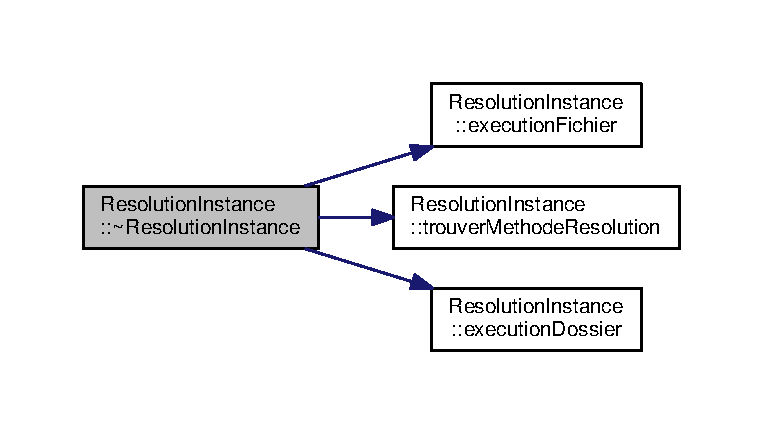
\includegraphics[width=350pt]{classResolutionInstance_acbc867c1e869aafcb0c20a5698e00aee_cgraph}
\end{center}
\end{figure}


\subsection{Member Function Documentation}
\mbox{\Hypertarget{classResolutionInstance_aa4184555e523d745accf570986f6fe45}\label{classResolutionInstance_aa4184555e523d745accf570986f6fe45}} 
\index{Resolution\+Instance@{Resolution\+Instance}!execution\+Dossier@{execution\+Dossier}}
\index{execution\+Dossier@{execution\+Dossier}!Resolution\+Instance@{Resolution\+Instance}}
\subsubsection{\texorpdfstring{execution\+Dossier()}{executionDossier()}}
{\footnotesize\ttfamily void Resolution\+Instance\+::execution\+Dossier (\begin{DoxyParamCaption}\item[{Q\+String}]{fichier\+Instance,  }\item[{Q\+String}]{type\+Resolution }\end{DoxyParamCaption})}



Execution de la résolution avec un seul fichier d\textquotesingle{}instance. 


\begin{DoxyParams}{Parameters}
{\em dossier\+Instance} & Chemin vers le dossier d\textquotesingle{}instances \\
\hline
{\em type\+Resolution} & Type de la résolution \\
\hline
\end{DoxyParams}
Here is the caller graph for this function\+:\nopagebreak
\begin{figure}[H]
\begin{center}
\leavevmode
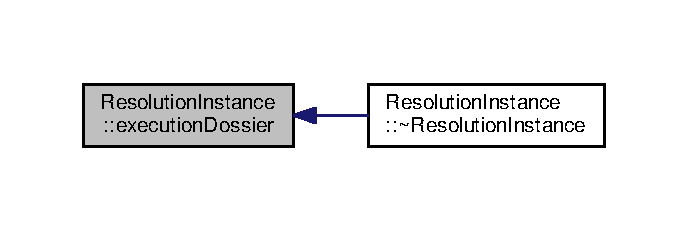
\includegraphics[width=330pt]{classResolutionInstance_aa4184555e523d745accf570986f6fe45_icgraph}
\end{center}
\end{figure}
\mbox{\Hypertarget{classResolutionInstance_a69b08f7877d8f12481f02bc31d1d391b}\label{classResolutionInstance_a69b08f7877d8f12481f02bc31d1d391b}} 
\index{Resolution\+Instance@{Resolution\+Instance}!execution\+Fichier@{execution\+Fichier}}
\index{execution\+Fichier@{execution\+Fichier}!Resolution\+Instance@{Resolution\+Instance}}
\subsubsection{\texorpdfstring{execution\+Fichier()}{executionFichier()}}
{\footnotesize\ttfamily void Resolution\+Instance\+::execution\+Fichier (\begin{DoxyParamCaption}\item[{Q\+String}]{fichier\+Instance,  }\item[{Q\+String}]{type\+Resolution }\end{DoxyParamCaption})}



Execution de la résolution avec un seul fichier d\textquotesingle{}instance. 


\begin{DoxyParams}{Parameters}
{\em fichier\+Instance} & Chemin vers le fichier d\textquotesingle{}instance \\
\hline
{\em type\+Resolution} & Type de la résolution \\
\hline
\end{DoxyParams}
Here is the caller graph for this function\+:\nopagebreak
\begin{figure}[H]
\begin{center}
\leavevmode
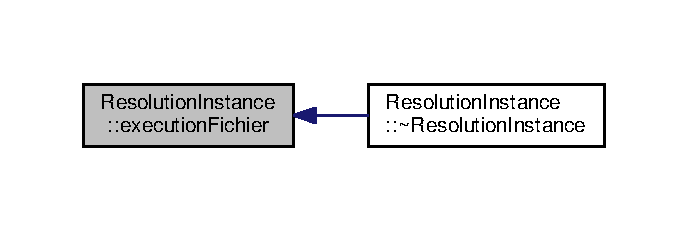
\includegraphics[width=330pt]{classResolutionInstance_a69b08f7877d8f12481f02bc31d1d391b_icgraph}
\end{center}
\end{figure}
\mbox{\Hypertarget{classResolutionInstance_a8e5aee07d5f05c978336c09379811aac}\label{classResolutionInstance_a8e5aee07d5f05c978336c09379811aac}} 
\index{Resolution\+Instance@{Resolution\+Instance}!trouver\+Methode\+Resolution@{trouver\+Methode\+Resolution}}
\index{trouver\+Methode\+Resolution@{trouver\+Methode\+Resolution}!Resolution\+Instance@{Resolution\+Instance}}
\subsubsection{\texorpdfstring{trouver\+Methode\+Resolution()}{trouverMethodeResolution()}}
{\footnotesize\ttfamily Q\+String Resolution\+Instance\+::trouver\+Methode\+Resolution (\begin{DoxyParamCaption}\item[{int}]{index\+Tableau,  }\item[{int}]{index\+Sous\+Element = {\ttfamily -\/1} }\end{DoxyParamCaption})}



Fonction permetant de trouver la methode de résolution suivant les champs Check\+Box remplis. 


\begin{DoxyParams}{Parameters}
{\em index\+Tableau} & Index du tableau selectionné \\
\hline
{\em index\+Sous\+Element} & Index du sous-\/élément du tableau selectionné (-\/1 si il n\textquotesingle{}y a pas de sous-\/élément) \\
\hline
\end{DoxyParams}
\begin{DoxyReturn}{Returns}
Q\+String La méthode de résolution 
\end{DoxyReturn}
Here is the caller graph for this function\+:\nopagebreak
\begin{figure}[H]
\begin{center}
\leavevmode
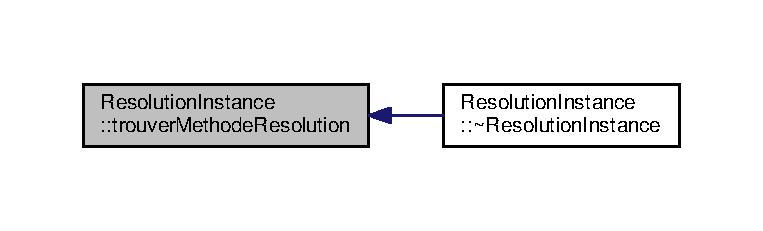
\includegraphics[width=350pt]{classResolutionInstance_a8e5aee07d5f05c978336c09379811aac_icgraph}
\end{center}
\end{figure}


The documentation for this class was generated from the following files\+:\begin{DoxyCompactItemize}
\item 
P\+R\+D\+Ordonancement/\hyperlink{resolutioninstance_8h}{resolutioninstance.\+h}\item 
P\+R\+D\+Ordonancement/\hyperlink{resolutioninstance_8cpp}{resolutioninstance.\+cpp}\end{DoxyCompactItemize}

\hypertarget{classWorkerComparaison}{}\section{Worker\+Comparaison Class Reference}
\label{classWorkerComparaison}\index{Worker\+Comparaison@{Worker\+Comparaison}}


Le Worker permetant de gérer la comparaison d\textquotesingle{}un dossier de résultats.  




{\ttfamily \#include $<$workercomparaison.\+h$>$}



Inheritance diagram for Worker\+Comparaison\+:
\nopagebreak
\begin{figure}[H]
\begin{center}
\leavevmode
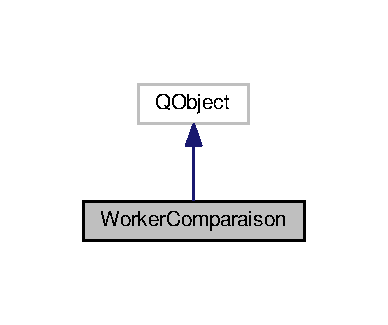
\includegraphics[width=186pt]{classWorkerComparaison__inherit__graph}
\end{center}
\end{figure}


Collaboration diagram for Worker\+Comparaison\+:
\nopagebreak
\begin{figure}[H]
\begin{center}
\leavevmode
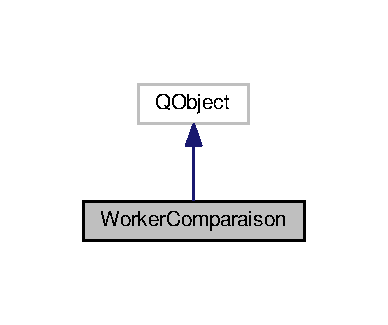
\includegraphics[width=186pt]{classWorkerComparaison__coll__graph}
\end{center}
\end{figure}
\subsection*{Public Slots}
\begin{DoxyCompactItemize}
\item 
void \hyperlink{classWorkerComparaison_ac62afd6b36f0c1590e5f3878334a9928}{process} ()
\begin{DoxyCompactList}\small\item\em Action effectuée lors du lancement du worker. \end{DoxyCompactList}\end{DoxyCompactItemize}
\subsection*{Signals}
\begin{DoxyCompactItemize}
\item 
void \hyperlink{classWorkerComparaison_a22ed9afba5f29d89a014b2b895d995b2}{finished} ()
\begin{DoxyCompactList}\small\item\em Action effectuée lorsque le worker a fini l\textquotesingle{}ensemble de ces tâches. \end{DoxyCompactList}\item 
void \hyperlink{classWorkerComparaison_aa9c167d230b850568f48575bc19241d7}{error} (Q\+String err)
\begin{DoxyCompactList}\small\item\em Action effectuée lorsqu\textquotesingle{}il y a une erreur dans le worker. \end{DoxyCompactList}\end{DoxyCompactItemize}
\subsection*{Public Member Functions}
\begin{DoxyCompactItemize}
\item 
\hyperlink{classWorkerComparaison_ab4c8a73500944f1e13c9008dd6302e80}{Worker\+Comparaison} (Q\+String dossier\+Resultat, Q\+String type\+Comparaison)
\begin{DoxyCompactList}\small\item\em Constructeur de la classe \hyperlink{classWorkerComparaison}{Worker\+Comparaison}. \end{DoxyCompactList}\item 
\hyperlink{classWorkerComparaison_a82acf722e3274431c0f86093c9dcb799}{$\sim$\+Worker\+Comparaison} ()
\begin{DoxyCompactList}\small\item\em Destructeur de la classe \hyperlink{classWorkerComparaison}{Worker\+Comparaison}. \end{DoxyCompactList}\end{DoxyCompactItemize}


\subsection{Detailed Description}
Le Worker permetant de gérer la comparaison d\textquotesingle{}un dossier de résultats. 

\subsection{Constructor \& Destructor Documentation}
\mbox{\Hypertarget{classWorkerComparaison_ab4c8a73500944f1e13c9008dd6302e80}\label{classWorkerComparaison_ab4c8a73500944f1e13c9008dd6302e80}} 
\index{Worker\+Comparaison@{Worker\+Comparaison}!Worker\+Comparaison@{Worker\+Comparaison}}
\index{Worker\+Comparaison@{Worker\+Comparaison}!Worker\+Comparaison@{Worker\+Comparaison}}
\subsubsection{\texorpdfstring{Worker\+Comparaison()}{WorkerComparaison()}}
{\footnotesize\ttfamily Worker\+Comparaison\+::\+Worker\+Comparaison (\begin{DoxyParamCaption}\item[{Q\+String}]{dossier\+Resultat,  }\item[{Q\+String}]{type\+Comparaison }\end{DoxyParamCaption})}



Constructeur de la classe \hyperlink{classWorkerComparaison}{Worker\+Comparaison}. 


\begin{DoxyParams}{Parameters}
{\em dossier\+Resultat} & Le chemin vers le dossier contenant les résultats des méthodes de résolution \\
\hline
{\em type\+Comparaison} & Le type de comparaison à effectuer \\
\hline
\end{DoxyParams}
\mbox{\Hypertarget{classWorkerComparaison_a82acf722e3274431c0f86093c9dcb799}\label{classWorkerComparaison_a82acf722e3274431c0f86093c9dcb799}} 
\index{Worker\+Comparaison@{Worker\+Comparaison}!````~Worker\+Comparaison@{$\sim$\+Worker\+Comparaison}}
\index{````~Worker\+Comparaison@{$\sim$\+Worker\+Comparaison}!Worker\+Comparaison@{Worker\+Comparaison}}
\subsubsection{\texorpdfstring{$\sim$\+Worker\+Comparaison()}{~WorkerComparaison()}}
{\footnotesize\ttfamily Worker\+Comparaison\+::$\sim$\+Worker\+Comparaison (\begin{DoxyParamCaption}{ }\end{DoxyParamCaption})}



Destructeur de la classe \hyperlink{classWorkerComparaison}{Worker\+Comparaison}. 



\subsection{Member Function Documentation}
\mbox{\Hypertarget{classWorkerComparaison_aa9c167d230b850568f48575bc19241d7}\label{classWorkerComparaison_aa9c167d230b850568f48575bc19241d7}} 
\index{Worker\+Comparaison@{Worker\+Comparaison}!error@{error}}
\index{error@{error}!Worker\+Comparaison@{Worker\+Comparaison}}
\subsubsection{\texorpdfstring{error}{error}}
{\footnotesize\ttfamily void Worker\+Comparaison\+::error (\begin{DoxyParamCaption}\item[{Q\+String}]{err }\end{DoxyParamCaption})\hspace{0.3cm}{\ttfamily [signal]}}



Action effectuée lorsqu\textquotesingle{}il y a une erreur dans le worker. 


\begin{DoxyParams}{Parameters}
{\em err} & \\
\hline
\end{DoxyParams}
\mbox{\Hypertarget{classWorkerComparaison_a22ed9afba5f29d89a014b2b895d995b2}\label{classWorkerComparaison_a22ed9afba5f29d89a014b2b895d995b2}} 
\index{Worker\+Comparaison@{Worker\+Comparaison}!finished@{finished}}
\index{finished@{finished}!Worker\+Comparaison@{Worker\+Comparaison}}
\subsubsection{\texorpdfstring{finished}{finished}}
{\footnotesize\ttfamily void Worker\+Comparaison\+::finished (\begin{DoxyParamCaption}{ }\end{DoxyParamCaption})\hspace{0.3cm}{\ttfamily [signal]}}



Action effectuée lorsque le worker a fini l\textquotesingle{}ensemble de ces tâches. 

Here is the caller graph for this function\+:
\nopagebreak
\begin{figure}[H]
\begin{center}
\leavevmode
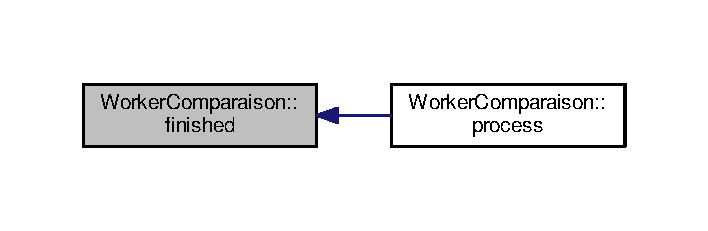
\includegraphics[width=340pt]{classWorkerComparaison_a22ed9afba5f29d89a014b2b895d995b2_icgraph}
\end{center}
\end{figure}
\mbox{\Hypertarget{classWorkerComparaison_ac62afd6b36f0c1590e5f3878334a9928}\label{classWorkerComparaison_ac62afd6b36f0c1590e5f3878334a9928}} 
\index{Worker\+Comparaison@{Worker\+Comparaison}!process@{process}}
\index{process@{process}!Worker\+Comparaison@{Worker\+Comparaison}}
\subsubsection{\texorpdfstring{process}{process}}
{\footnotesize\ttfamily void Worker\+Comparaison\+::process (\begin{DoxyParamCaption}{ }\end{DoxyParamCaption})\hspace{0.3cm}{\ttfamily [slot]}}



Action effectuée lors du lancement du worker. 



The documentation for this class was generated from the following files\+:\begin{DoxyCompactItemize}
\item 
P\+R\+D\+Ordonancement/\hyperlink{workercomparaison_8h}{workercomparaison.\+h}\item 
P\+R\+D\+Ordonancement/\hyperlink{workercomparaison_8cpp}{workercomparaison.\+cpp}\end{DoxyCompactItemize}

\hypertarget{classWorkerDossier}{}\section{Worker\+Dossier Class Reference}
\label{classWorkerDossier}\index{Worker\+Dossier@{Worker\+Dossier}}


Le Worker permetant de gérer la résolution d\textquotesingle{}un dossier d\textquotesingle{}instances.  




{\ttfamily \#include $<$workerdossier.\+h$>$}



Inheritance diagram for Worker\+Dossier\+:\nopagebreak
\begin{figure}[H]
\begin{center}
\leavevmode
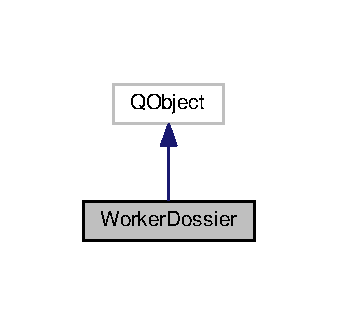
\includegraphics[width=162pt]{classWorkerDossier__inherit__graph}
\end{center}
\end{figure}


Collaboration diagram for Worker\+Dossier\+:\nopagebreak
\begin{figure}[H]
\begin{center}
\leavevmode
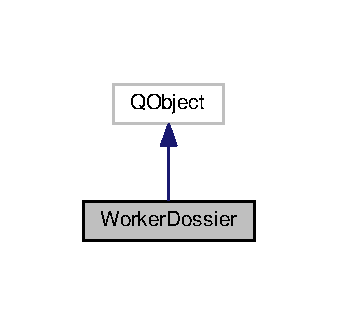
\includegraphics[width=162pt]{classWorkerDossier__coll__graph}
\end{center}
\end{figure}
\subsection*{Public Slots}
\begin{DoxyCompactItemize}
\item 
void \hyperlink{classWorkerDossier_a2e2970df6c43c669eb730a858a780a31}{process} ()
\begin{DoxyCompactList}\small\item\em Action effectuée lors du lancement du worker. \end{DoxyCompactList}\end{DoxyCompactItemize}
\subsection*{Signals}
\begin{DoxyCompactItemize}
\item 
void \hyperlink{classWorkerDossier_aef696bfd03c464295dc80fb1fc9f71da}{finished} ()
\begin{DoxyCompactList}\small\item\em Action effectuée lorsque le worker a fini l\textquotesingle{}ensemble de ces tâches. \end{DoxyCompactList}\item 
void \hyperlink{classWorkerDossier_afb02d04b47bb81450661cbc36ad25902}{error} (Q\+String err)
\begin{DoxyCompactList}\small\item\em Action effectuée lorsqu\textquotesingle{}il y a une erreur dans le worker. \end{DoxyCompactList}\end{DoxyCompactItemize}
\subsection*{Public Member Functions}
\begin{DoxyCompactItemize}
\item 
\hyperlink{classWorkerDossier_ae62defa93ef94862572fda95736a03ed}{Worker\+Dossier} (Q\+String dossier\+Instance, Q\+String type\+Resolution)
\begin{DoxyCompactList}\small\item\em Constructeur de la classe \hyperlink{classWorkerDossier}{Worker\+Dossier}. \end{DoxyCompactList}\item 
\hyperlink{classWorkerDossier_ac2d339dcdd7e35d1fed6debf3495f904}{$\sim$\+Worker\+Dossier} ()
\begin{DoxyCompactList}\small\item\em Destructeur de la classe \hyperlink{classWorkerDossier}{Worker\+Dossier}. \end{DoxyCompactList}\end{DoxyCompactItemize}


\subsection{Detailed Description}
Le Worker permetant de gérer la résolution d\textquotesingle{}un dossier d\textquotesingle{}instances. 

\subsection{Constructor \& Destructor Documentation}
\mbox{\Hypertarget{classWorkerDossier_ae62defa93ef94862572fda95736a03ed}\label{classWorkerDossier_ae62defa93ef94862572fda95736a03ed}} 
\index{Worker\+Dossier@{Worker\+Dossier}!Worker\+Dossier@{Worker\+Dossier}}
\index{Worker\+Dossier@{Worker\+Dossier}!Worker\+Dossier@{Worker\+Dossier}}
\subsubsection{\texorpdfstring{Worker\+Dossier()}{WorkerDossier()}}
{\footnotesize\ttfamily Worker\+Dossier\+::\+Worker\+Dossier (\begin{DoxyParamCaption}\item[{Q\+String}]{dossier\+Instance,  }\item[{Q\+String}]{type\+Resolution }\end{DoxyParamCaption})}



Constructeur de la classe \hyperlink{classWorkerDossier}{Worker\+Dossier}. 


\begin{DoxyParams}{Parameters}
{\em dossier\+Instance} & Le chemin vers le dossier d\textquotesingle{}instance \\
\hline
{\em type\+Resolution} & Le type de résolution à effectuer \\
\hline
\end{DoxyParams}
\mbox{\Hypertarget{classWorkerDossier_ac2d339dcdd7e35d1fed6debf3495f904}\label{classWorkerDossier_ac2d339dcdd7e35d1fed6debf3495f904}} 
\index{Worker\+Dossier@{Worker\+Dossier}!````~Worker\+Dossier@{$\sim$\+Worker\+Dossier}}
\index{````~Worker\+Dossier@{$\sim$\+Worker\+Dossier}!Worker\+Dossier@{Worker\+Dossier}}
\subsubsection{\texorpdfstring{$\sim$\+Worker\+Dossier()}{~WorkerDossier()}}
{\footnotesize\ttfamily Worker\+Dossier\+::$\sim$\+Worker\+Dossier (\begin{DoxyParamCaption}{ }\end{DoxyParamCaption})}



Destructeur de la classe \hyperlink{classWorkerDossier}{Worker\+Dossier}. 



\subsection{Member Function Documentation}
\mbox{\Hypertarget{classWorkerDossier_afb02d04b47bb81450661cbc36ad25902}\label{classWorkerDossier_afb02d04b47bb81450661cbc36ad25902}} 
\index{Worker\+Dossier@{Worker\+Dossier}!error@{error}}
\index{error@{error}!Worker\+Dossier@{Worker\+Dossier}}
\subsubsection{\texorpdfstring{error}{error}}
{\footnotesize\ttfamily void Worker\+Dossier\+::error (\begin{DoxyParamCaption}\item[{Q\+String}]{err }\end{DoxyParamCaption})\hspace{0.3cm}{\ttfamily [signal]}}



Action effectuée lorsqu\textquotesingle{}il y a une erreur dans le worker. 


\begin{DoxyParams}{Parameters}
{\em err} & \\
\hline
\end{DoxyParams}
\mbox{\Hypertarget{classWorkerDossier_aef696bfd03c464295dc80fb1fc9f71da}\label{classWorkerDossier_aef696bfd03c464295dc80fb1fc9f71da}} 
\index{Worker\+Dossier@{Worker\+Dossier}!finished@{finished}}
\index{finished@{finished}!Worker\+Dossier@{Worker\+Dossier}}
\subsubsection{\texorpdfstring{finished}{finished}}
{\footnotesize\ttfamily void Worker\+Dossier\+::finished (\begin{DoxyParamCaption}{ }\end{DoxyParamCaption})\hspace{0.3cm}{\ttfamily [signal]}}



Action effectuée lorsque le worker a fini l\textquotesingle{}ensemble de ces tâches. 

Here is the caller graph for this function\+:\nopagebreak
\begin{figure}[H]
\begin{center}
\leavevmode
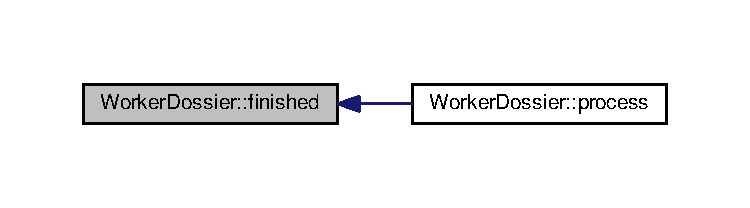
\includegraphics[width=350pt]{classWorkerDossier_aef696bfd03c464295dc80fb1fc9f71da_icgraph}
\end{center}
\end{figure}
\mbox{\Hypertarget{classWorkerDossier_a2e2970df6c43c669eb730a858a780a31}\label{classWorkerDossier_a2e2970df6c43c669eb730a858a780a31}} 
\index{Worker\+Dossier@{Worker\+Dossier}!process@{process}}
\index{process@{process}!Worker\+Dossier@{Worker\+Dossier}}
\subsubsection{\texorpdfstring{process}{process}}
{\footnotesize\ttfamily void Worker\+Dossier\+::process (\begin{DoxyParamCaption}{ }\end{DoxyParamCaption})\hspace{0.3cm}{\ttfamily [slot]}}



Action effectuée lors du lancement du worker. 

Here is the call graph for this function\+:\nopagebreak
\begin{figure}[H]
\begin{center}
\leavevmode
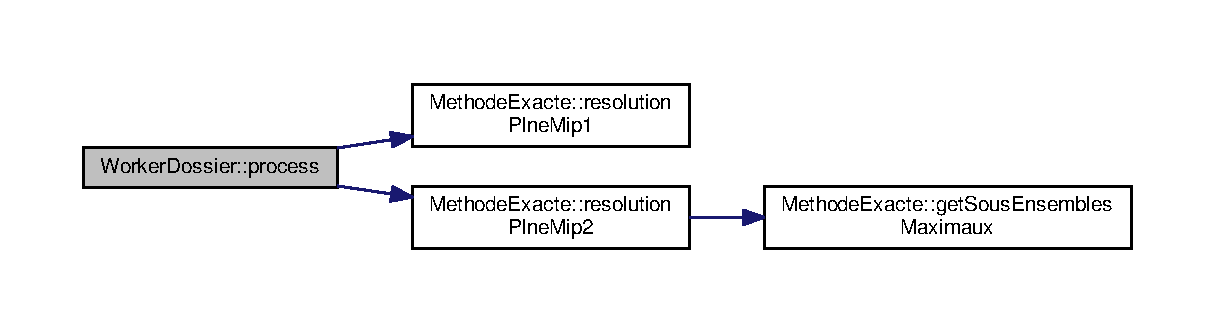
\includegraphics[width=350pt]{classWorkerDossier_a2e2970df6c43c669eb730a858a780a31_cgraph}
\end{center}
\end{figure}


The documentation for this class was generated from the following files\+:\begin{DoxyCompactItemize}
\item 
P\+R\+D\+Ordonancement/\hyperlink{workerdossier_8h}{workerdossier.\+h}\item 
P\+R\+D\+Ordonancement/\hyperlink{workerdossier_8cpp}{workerdossier.\+cpp}\end{DoxyCompactItemize}

\hypertarget{classWorkerFichier}{}\section{Worker\+Fichier Class Reference}
\label{classWorkerFichier}\index{Worker\+Fichier@{Worker\+Fichier}}


Le Worker permetant de gérer la résolution d\textquotesingle{}un fichier d\textquotesingle{}instance.  




{\ttfamily \#include $<$workerfichier.\+h$>$}



Inheritance diagram for Worker\+Fichier\+:\nopagebreak
\begin{figure}[H]
\begin{center}
\leavevmode
\includegraphics[width=157pt]{classWorkerFichier__inherit__graph}
\end{center}
\end{figure}


Collaboration diagram for Worker\+Fichier\+:\nopagebreak
\begin{figure}[H]
\begin{center}
\leavevmode
\includegraphics[width=157pt]{classWorkerFichier__coll__graph}
\end{center}
\end{figure}
\subsection*{Public Slots}
\begin{DoxyCompactItemize}
\item 
void \hyperlink{classWorkerFichier_a3b72efa3a7e2de6f1a8001d999731e11}{process} ()
\begin{DoxyCompactList}\small\item\em Action effectuée lors du lancement du worker. \end{DoxyCompactList}\end{DoxyCompactItemize}
\subsection*{Signals}
\begin{DoxyCompactItemize}
\item 
void \hyperlink{classWorkerFichier_a829c3872070e4cab2d84c11b7c12dccc}{finished} ()
\begin{DoxyCompactList}\small\item\em Action effectuée lorsque le worker a fini l\textquotesingle{}ensemble de ces tâches. \end{DoxyCompactList}\item 
void \hyperlink{classWorkerFichier_ae7f4b3f3ce2a053855a21d05f13e1f4e}{error} (Q\+String err)
\begin{DoxyCompactList}\small\item\em Action effectuée lorsqu\textquotesingle{}il y a une erreur dans le worker. \end{DoxyCompactList}\end{DoxyCompactItemize}
\subsection*{Public Member Functions}
\begin{DoxyCompactItemize}
\item 
\hyperlink{classWorkerFichier_a9ec0e174cceef123487826fb902fb649}{Worker\+Fichier} (Q\+String fichier\+Instance, Q\+String type\+Resolution)
\begin{DoxyCompactList}\small\item\em Constructeur de la classe \hyperlink{classWorkerFichier}{Worker\+Fichier}. \end{DoxyCompactList}\item 
\hyperlink{classWorkerFichier_acabdd12b795f6b7f656e0ed9e61cb6ca}{$\sim$\+Worker\+Fichier} ()
\begin{DoxyCompactList}\small\item\em Destructeur de la classe \hyperlink{classWorkerFichier}{Worker\+Fichier}. \end{DoxyCompactList}\end{DoxyCompactItemize}


\subsection{Detailed Description}
Le Worker permetant de gérer la résolution d\textquotesingle{}un fichier d\textquotesingle{}instance. 

\subsection{Constructor \& Destructor Documentation}
\mbox{\Hypertarget{classWorkerFichier_a9ec0e174cceef123487826fb902fb649}\label{classWorkerFichier_a9ec0e174cceef123487826fb902fb649}} 
\index{Worker\+Fichier@{Worker\+Fichier}!Worker\+Fichier@{Worker\+Fichier}}
\index{Worker\+Fichier@{Worker\+Fichier}!Worker\+Fichier@{Worker\+Fichier}}
\subsubsection{\texorpdfstring{Worker\+Fichier()}{WorkerFichier()}}
{\footnotesize\ttfamily Worker\+Fichier\+::\+Worker\+Fichier (\begin{DoxyParamCaption}\item[{Q\+String}]{fichier\+Instance,  }\item[{Q\+String}]{type\+Resolution }\end{DoxyParamCaption})}



Constructeur de la classe \hyperlink{classWorkerFichier}{Worker\+Fichier}. 


\begin{DoxyParams}{Parameters}
{\em fichier\+Instance} & Le chemin vers le fichier d\textquotesingle{}instance \\
\hline
{\em type\+Resolution} & Le type de résolution à effectuer \\
\hline
\end{DoxyParams}
\mbox{\Hypertarget{classWorkerFichier_acabdd12b795f6b7f656e0ed9e61cb6ca}\label{classWorkerFichier_acabdd12b795f6b7f656e0ed9e61cb6ca}} 
\index{Worker\+Fichier@{Worker\+Fichier}!````~Worker\+Fichier@{$\sim$\+Worker\+Fichier}}
\index{````~Worker\+Fichier@{$\sim$\+Worker\+Fichier}!Worker\+Fichier@{Worker\+Fichier}}
\subsubsection{\texorpdfstring{$\sim$\+Worker\+Fichier()}{~WorkerFichier()}}
{\footnotesize\ttfamily Worker\+Fichier\+::$\sim$\+Worker\+Fichier (\begin{DoxyParamCaption}{ }\end{DoxyParamCaption})}



Destructeur de la classe \hyperlink{classWorkerFichier}{Worker\+Fichier}. 



\subsection{Member Function Documentation}
\mbox{\Hypertarget{classWorkerFichier_ae7f4b3f3ce2a053855a21d05f13e1f4e}\label{classWorkerFichier_ae7f4b3f3ce2a053855a21d05f13e1f4e}} 
\index{Worker\+Fichier@{Worker\+Fichier}!error@{error}}
\index{error@{error}!Worker\+Fichier@{Worker\+Fichier}}
\subsubsection{\texorpdfstring{error}{error}}
{\footnotesize\ttfamily void Worker\+Fichier\+::error (\begin{DoxyParamCaption}\item[{Q\+String}]{err }\end{DoxyParamCaption})\hspace{0.3cm}{\ttfamily [signal]}}



Action effectuée lorsqu\textquotesingle{}il y a une erreur dans le worker. 


\begin{DoxyParams}{Parameters}
{\em err} & \\
\hline
\end{DoxyParams}
\mbox{\Hypertarget{classWorkerFichier_a829c3872070e4cab2d84c11b7c12dccc}\label{classWorkerFichier_a829c3872070e4cab2d84c11b7c12dccc}} 
\index{Worker\+Fichier@{Worker\+Fichier}!finished@{finished}}
\index{finished@{finished}!Worker\+Fichier@{Worker\+Fichier}}
\subsubsection{\texorpdfstring{finished}{finished}}
{\footnotesize\ttfamily void Worker\+Fichier\+::finished (\begin{DoxyParamCaption}{ }\end{DoxyParamCaption})\hspace{0.3cm}{\ttfamily [signal]}}



Action effectuée lorsque le worker a fini l\textquotesingle{}ensemble de ces tâches. 

Here is the caller graph for this function\+:\nopagebreak
\begin{figure}[H]
\begin{center}
\leavevmode
\includegraphics[width=350pt]{classWorkerFichier_a829c3872070e4cab2d84c11b7c12dccc_icgraph}
\end{center}
\end{figure}
\mbox{\Hypertarget{classWorkerFichier_a3b72efa3a7e2de6f1a8001d999731e11}\label{classWorkerFichier_a3b72efa3a7e2de6f1a8001d999731e11}} 
\index{Worker\+Fichier@{Worker\+Fichier}!process@{process}}
\index{process@{process}!Worker\+Fichier@{Worker\+Fichier}}
\subsubsection{\texorpdfstring{process}{process}}
{\footnotesize\ttfamily void Worker\+Fichier\+::process (\begin{DoxyParamCaption}{ }\end{DoxyParamCaption})\hspace{0.3cm}{\ttfamily [slot]}}



Action effectuée lors du lancement du worker. 

Here is the call graph for this function\+:\nopagebreak
\begin{figure}[H]
\begin{center}
\leavevmode
\includegraphics[width=350pt]{classWorkerFichier_a3b72efa3a7e2de6f1a8001d999731e11_cgraph}
\end{center}
\end{figure}


The documentation for this class was generated from the following files\+:\begin{DoxyCompactItemize}
\item 
P\+R\+D\+Ordonancement/\hyperlink{workerfichier_8h}{workerfichier.\+h}\item 
P\+R\+D\+Ordonancement/\hyperlink{workerfichier_8cpp}{workerfichier.\+cpp}\end{DoxyCompactItemize}

\hypertarget{classWorkerInstance}{}\section{Worker\+Instance Class Reference}
\label{classWorkerInstance}\index{Worker\+Instance@{Worker\+Instance}}


Le Worker permetant de gérer la génération de fichiers d\textquotesingle{}instance.  




{\ttfamily \#include $<$workerinstance.\+h$>$}



Inheritance diagram for Worker\+Instance\+:\nopagebreak
\begin{figure}[H]
\begin{center}
\leavevmode
\includegraphics[width=166pt]{classWorkerInstance__inherit__graph}
\end{center}
\end{figure}


Collaboration diagram for Worker\+Instance\+:\nopagebreak
\begin{figure}[H]
\begin{center}
\leavevmode
\includegraphics[width=166pt]{classWorkerInstance__coll__graph}
\end{center}
\end{figure}
\subsection*{Public Slots}
\begin{DoxyCompactItemize}
\item 
void \hyperlink{classWorkerInstance_ab9005529d8aa529d74226d8e4a1e9f3f}{process} ()
\begin{DoxyCompactList}\small\item\em Action effectuée lors du lancement du worker. \end{DoxyCompactList}\end{DoxyCompactItemize}
\subsection*{Signals}
\begin{DoxyCompactItemize}
\item 
void \hyperlink{classWorkerInstance_ac9e45034de2450472fcc07ba0b960000}{finished} ()
\begin{DoxyCompactList}\small\item\em Action effectuée lorsque le worker a fini l\textquotesingle{}ensemble de ces tâches. \end{DoxyCompactList}\item 
void \hyperlink{classWorkerInstance_a7327b868e3d96daa63e71c47076e598e}{error} (Q\+String err)
\begin{DoxyCompactList}\small\item\em Action effectuée lorsqu\textquotesingle{}il y a une erreur dans le worker. \end{DoxyCompactList}\end{DoxyCompactItemize}
\subsection*{Public Member Functions}
\begin{DoxyCompactItemize}
\item 
\hyperlink{classWorkerInstance_ab9f399d25e9e1d7f7387a6c1d47da835}{Worker\+Instance} (unsigned int nbr\+Instance, unsigned int nbr\+Jobs, unsigned int nbr\+Ressources, unsigned int nbr\+Machines, unsigned int horizon\+Planification)
\begin{DoxyCompactList}\small\item\em Constructeur de la classe \hyperlink{classWorkerInstance}{Worker\+Instance}. \end{DoxyCompactList}\item 
\hyperlink{classWorkerInstance_a0072f72256aacba8cb97ab4f50bcb939}{$\sim$\+Worker\+Instance} ()
\begin{DoxyCompactList}\small\item\em Destructeur de la classe \hyperlink{classWorkerInstance}{Worker\+Instance}. \end{DoxyCompactList}\end{DoxyCompactItemize}


\subsection{Detailed Description}
Le Worker permetant de gérer la génération de fichiers d\textquotesingle{}instance. 

\subsection{Constructor \& Destructor Documentation}
\mbox{\Hypertarget{classWorkerInstance_ab9f399d25e9e1d7f7387a6c1d47da835}\label{classWorkerInstance_ab9f399d25e9e1d7f7387a6c1d47da835}} 
\index{Worker\+Instance@{Worker\+Instance}!Worker\+Instance@{Worker\+Instance}}
\index{Worker\+Instance@{Worker\+Instance}!Worker\+Instance@{Worker\+Instance}}
\subsubsection{\texorpdfstring{Worker\+Instance()}{WorkerInstance()}}
{\footnotesize\ttfamily Worker\+Instance\+::\+Worker\+Instance (\begin{DoxyParamCaption}\item[{unsigned int}]{nbr\+Instance,  }\item[{unsigned int}]{nbr\+Jobs,  }\item[{unsigned int}]{nbr\+Ressources,  }\item[{unsigned int}]{nbr\+Machines,  }\item[{unsigned int}]{horizon\+Planification }\end{DoxyParamCaption})}



Constructeur de la classe \hyperlink{classWorkerInstance}{Worker\+Instance}. 


\begin{DoxyParams}{Parameters}
{\em nbr\+Instance} & Le nombre d\textquotesingle{}instance à générer \\
\hline
{\em nbr\+Jobs} & Le nombre de jobs par instance \\
\hline
{\em nbr\+Ressources} & Le nombre de ressources par instance \\
\hline
{\em nbr\+Machines} & Le nombre de machines par instance \\
\hline
{\em horizon\+Planification} & L\textquotesingle{}horizon maximale de planification par instance \\
\hline
\end{DoxyParams}
\mbox{\Hypertarget{classWorkerInstance_a0072f72256aacba8cb97ab4f50bcb939}\label{classWorkerInstance_a0072f72256aacba8cb97ab4f50bcb939}} 
\index{Worker\+Instance@{Worker\+Instance}!````~Worker\+Instance@{$\sim$\+Worker\+Instance}}
\index{````~Worker\+Instance@{$\sim$\+Worker\+Instance}!Worker\+Instance@{Worker\+Instance}}
\subsubsection{\texorpdfstring{$\sim$\+Worker\+Instance()}{~WorkerInstance()}}
{\footnotesize\ttfamily Worker\+Instance\+::$\sim$\+Worker\+Instance (\begin{DoxyParamCaption}{ }\end{DoxyParamCaption})}



Destructeur de la classe \hyperlink{classWorkerInstance}{Worker\+Instance}. 



\subsection{Member Function Documentation}
\mbox{\Hypertarget{classWorkerInstance_a7327b868e3d96daa63e71c47076e598e}\label{classWorkerInstance_a7327b868e3d96daa63e71c47076e598e}} 
\index{Worker\+Instance@{Worker\+Instance}!error@{error}}
\index{error@{error}!Worker\+Instance@{Worker\+Instance}}
\subsubsection{\texorpdfstring{error}{error}}
{\footnotesize\ttfamily void Worker\+Instance\+::error (\begin{DoxyParamCaption}\item[{Q\+String}]{err }\end{DoxyParamCaption})\hspace{0.3cm}{\ttfamily [signal]}}



Action effectuée lorsqu\textquotesingle{}il y a une erreur dans le worker. 


\begin{DoxyParams}{Parameters}
{\em err} & \\
\hline
\end{DoxyParams}
\mbox{\Hypertarget{classWorkerInstance_ac9e45034de2450472fcc07ba0b960000}\label{classWorkerInstance_ac9e45034de2450472fcc07ba0b960000}} 
\index{Worker\+Instance@{Worker\+Instance}!finished@{finished}}
\index{finished@{finished}!Worker\+Instance@{Worker\+Instance}}
\subsubsection{\texorpdfstring{finished}{finished}}
{\footnotesize\ttfamily void Worker\+Instance\+::finished (\begin{DoxyParamCaption}{ }\end{DoxyParamCaption})\hspace{0.3cm}{\ttfamily [signal]}}



Action effectuée lorsque le worker a fini l\textquotesingle{}ensemble de ces tâches. 

Here is the caller graph for this function\+:\nopagebreak
\begin{figure}[H]
\begin{center}
\leavevmode
\includegraphics[width=350pt]{classWorkerInstance_ac9e45034de2450472fcc07ba0b960000_icgraph}
\end{center}
\end{figure}
\mbox{\Hypertarget{classWorkerInstance_ab9005529d8aa529d74226d8e4a1e9f3f}\label{classWorkerInstance_ab9005529d8aa529d74226d8e4a1e9f3f}} 
\index{Worker\+Instance@{Worker\+Instance}!process@{process}}
\index{process@{process}!Worker\+Instance@{Worker\+Instance}}
\subsubsection{\texorpdfstring{process}{process}}
{\footnotesize\ttfamily void Worker\+Instance\+::process (\begin{DoxyParamCaption}{ }\end{DoxyParamCaption})\hspace{0.3cm}{\ttfamily [slot]}}



Action effectuée lors du lancement du worker. 

Here is the call graph for this function\+:\nopagebreak
\begin{figure}[H]
\begin{center}
\leavevmode
\includegraphics[width=350pt]{classWorkerInstance_ab9005529d8aa529d74226d8e4a1e9f3f_cgraph}
\end{center}
\end{figure}


The documentation for this class was generated from the following files\+:\begin{DoxyCompactItemize}
\item 
P\+R\+D\+Ordonancement/\hyperlink{workerinstance_8h}{workerinstance.\+h}\item 
P\+R\+D\+Ordonancement/\hyperlink{workerinstance_8cpp}{workerinstance.\+cpp}\end{DoxyCompactItemize}

\chapter{File Documentation}
\hypertarget{comparaisonsolution_8cpp}{}\section{P\+R\+D\+Ordonancement/comparaisonsolution.cpp File Reference}
\label{comparaisonsolution_8cpp}\index{P\+R\+D\+Ordonancement/comparaisonsolution.\+cpp@{P\+R\+D\+Ordonancement/comparaisonsolution.\+cpp}}
{\ttfamily \#include \char`\"{}comparaisonsolution.\+h\char`\"{}}\newline
{\ttfamily \#include \char`\"{}ui\+\_\+comparaisonsolution.\+h\char`\"{}}\newline
Include dependency graph for comparaisonsolution.\+cpp\+:
\nopagebreak
\begin{figure}[H]
\begin{center}
\leavevmode
\includegraphics[width=350pt]{comparaisonsolution_8cpp__incl}
\end{center}
\end{figure}

\hypertarget{comparaisonsolution_8h}{}\section{P\+R\+D\+Ordonancement/comparaisonsolution.h File Reference}
\label{comparaisonsolution_8h}\index{P\+R\+D\+Ordonancement/comparaisonsolution.\+h@{P\+R\+D\+Ordonancement/comparaisonsolution.\+h}}
{\ttfamily \#include $<$Q\+Dialog$>$}\newline
{\ttfamily \#include $<$Q\+File\+Dialog$>$}\newline
{\ttfamily \#include $<$Q\+File\+Info$>$}\newline
{\ttfamily \#include $<$Qt\+Concurrent/\+Qt\+Concurrent$>$}\newline
{\ttfamily \#include \char`\"{}workercomparaison.\+h\char`\"{}}\newline
Include dependency graph for comparaisonsolution.\+h\+:\nopagebreak
\begin{figure}[H]
\begin{center}
\leavevmode
\includegraphics[width=350pt]{comparaisonsolution_8h__incl}
\end{center}
\end{figure}
This graph shows which files directly or indirectly include this file\+:\nopagebreak
\begin{figure}[H]
\begin{center}
\leavevmode
\includegraphics[width=350pt]{comparaisonsolution_8h__dep__incl}
\end{center}
\end{figure}
\subsection*{Classes}
\begin{DoxyCompactItemize}
\item 
class \hyperlink{classComparaisonSolution}{Comparaison\+Solution}
\end{DoxyCompactItemize}
\subsection*{Namespaces}
\begin{DoxyCompactItemize}
\item 
 \hyperlink{namespaceUi}{Ui}
\end{DoxyCompactItemize}

\hypertarget{creationinstance_8cpp}{}\section{P\+R\+D\+Ordonancement/creationinstance.cpp File Reference}
\label{creationinstance_8cpp}\index{P\+R\+D\+Ordonancement/creationinstance.\+cpp@{P\+R\+D\+Ordonancement/creationinstance.\+cpp}}
{\ttfamily \#include \char`\"{}creationinstance.\+h\char`\"{}}\newline
Include dependency graph for creationinstance.\+cpp\+:\nopagebreak
\begin{figure}[H]
\begin{center}
\leavevmode
\includegraphics[width=280pt]{creationinstance_8cpp__incl}
\end{center}
\end{figure}

\hypertarget{creationinstance_8h}{}\section{P\+R\+D\+Ordonancement/creationinstance.h File Reference}
\label{creationinstance_8h}\index{P\+R\+D\+Ordonancement/creationinstance.\+h@{P\+R\+D\+Ordonancement/creationinstance.\+h}}
This graph shows which files directly or indirectly include this file\+:\nopagebreak
\begin{figure}[H]
\begin{center}
\leavevmode
\includegraphics[width=280pt]{creationinstance_8h__dep__incl}
\end{center}
\end{figure}
\subsection*{Classes}
\begin{DoxyCompactItemize}
\item 
class \hyperlink{classCreationInstance}{Creation\+Instance}
\end{DoxyCompactItemize}

\hypertarget{fenetreprincipale_8cpp}{}\section{P\+R\+D\+Ordonancement/fenetreprincipale.cpp File Reference}
\label{fenetreprincipale_8cpp}\index{P\+R\+D\+Ordonancement/fenetreprincipale.\+cpp@{P\+R\+D\+Ordonancement/fenetreprincipale.\+cpp}}
{\ttfamily \#include \char`\"{}fenetreprincipale.\+h\char`\"{}}\newline
{\ttfamily \#include \char`\"{}ui\+\_\+fenetreprincipale.\+h\char`\"{}}\newline
Include dependency graph for fenetreprincipale.\+cpp\+:
\nopagebreak
\begin{figure}[H]
\begin{center}
\leavevmode
\includegraphics[width=350pt]{fenetreprincipale_8cpp__incl}
\end{center}
\end{figure}

\hypertarget{fenetreprincipale_8h}{}\section{P\+R\+D\+Ordonancement/fenetreprincipale.h File Reference}
\label{fenetreprincipale_8h}\index{P\+R\+D\+Ordonancement/fenetreprincipale.\+h@{P\+R\+D\+Ordonancement/fenetreprincipale.\+h}}
{\ttfamily \#include $<$Q\+Main\+Window$>$}\newline
{\ttfamily \#include \char`\"{}generationinstance.\+h\char`\"{}}\newline
{\ttfamily \#include \char`\"{}resolutioninstance.\+h\char`\"{}}\newline
{\ttfamily \#include \char`\"{}comparaisonsolution.\+h\char`\"{}}\newline
Include dependency graph for fenetreprincipale.\+h\+:
\nopagebreak
\begin{figure}[H]
\begin{center}
\leavevmode
\includegraphics[width=350pt]{fenetreprincipale_8h__incl}
\end{center}
\end{figure}
This graph shows which files directly or indirectly include this file\+:\nopagebreak
\begin{figure}[H]
\begin{center}
\leavevmode
\includegraphics[width=350pt]{fenetreprincipale_8h__dep__incl}
\end{center}
\end{figure}
\subsection*{Classes}
\begin{DoxyCompactItemize}
\item 
class \hyperlink{classFenetrePrincipale}{Fenetre\+Principale}
\begin{DoxyCompactList}\small\item\em La Fenêtre Principale. \end{DoxyCompactList}\end{DoxyCompactItemize}
\subsection*{Namespaces}
\begin{DoxyCompactItemize}
\item 
 \hyperlink{namespaceUi}{Ui}
\end{DoxyCompactItemize}

\hypertarget{generationinstance_8cpp}{}\section{P\+R\+D\+Ordonancement/generationinstance.cpp File Reference}
\label{generationinstance_8cpp}\index{P\+R\+D\+Ordonancement/generationinstance.\+cpp@{P\+R\+D\+Ordonancement/generationinstance.\+cpp}}
{\ttfamily \#include \char`\"{}generationinstance.\+h\char`\"{}}\newline
{\ttfamily \#include \char`\"{}ui\+\_\+generationinstance.\+h\char`\"{}}\newline
{\ttfamily \#include \char`\"{}Q\+Message\+Box\char`\"{}}\newline
Include dependency graph for generationinstance.\+cpp\+:\nopagebreak
\begin{figure}[H]
\begin{center}
\leavevmode
\includegraphics[width=350pt]{generationinstance_8cpp__incl}
\end{center}
\end{figure}

\hypertarget{generationinstance_8h}{}\section{P\+R\+D\+Ordonancement/generationinstance.h File Reference}
\label{generationinstance_8h}\index{P\+R\+D\+Ordonancement/generationinstance.\+h@{P\+R\+D\+Ordonancement/generationinstance.\+h}}
{\ttfamily \#include $<$Q\+Dialog$>$}\newline
{\ttfamily \#include \char`\"{}workerinstance.\+h\char`\"{}}\newline
{\ttfamily \#include $<$Qt\+Concurrent/\+Qt\+Concurrent$>$}\newline
{\ttfamily \#include $<$iostream$>$}\newline
{\ttfamily \#include \char`\"{}Q\+Message\+Box\char`\"{}}\newline
Include dependency graph for generationinstance.\+h\+:\nopagebreak
\begin{figure}[H]
\begin{center}
\leavevmode
\includegraphics[width=350pt]{generationinstance_8h__incl}
\end{center}
\end{figure}
This graph shows which files directly or indirectly include this file\+:\nopagebreak
\begin{figure}[H]
\begin{center}
\leavevmode
\includegraphics[width=350pt]{generationinstance_8h__dep__incl}
\end{center}
\end{figure}
\subsection*{Classes}
\begin{DoxyCompactItemize}
\item 
class \hyperlink{classGenerationInstance}{Generation\+Instance}
\begin{DoxyCompactList}\small\item\em La fenêtre de génération d\textquotesingle{}instance. \end{DoxyCompactList}\end{DoxyCompactItemize}
\subsection*{Namespaces}
\begin{DoxyCompactItemize}
\item 
 \hyperlink{namespaceUi}{Ui}
\end{DoxyCompactItemize}

\hypertarget{heuristique_8cpp}{}\section{P\+R\+D\+Ordonancement/heuristique.cpp File Reference}
\label{heuristique_8cpp}\index{P\+R\+D\+Ordonancement/heuristique.\+cpp@{P\+R\+D\+Ordonancement/heuristique.\+cpp}}
{\ttfamily \#include \char`\"{}heuristique.\+h\char`\"{}}\newline
Include dependency graph for heuristique.\+cpp\+:\nopagebreak
\begin{figure}[H]
\begin{center}
\leavevmode
\includegraphics[width=350pt]{heuristique_8cpp__incl}
\end{center}
\end{figure}

\hypertarget{heuristique_8h}{}\section{P\+R\+D\+Ordonancement/heuristique.h File Reference}
\label{heuristique_8h}\index{P\+R\+D\+Ordonancement/heuristique.\+h@{P\+R\+D\+Ordonancement/heuristique.\+h}}
{\ttfamily \#include $<$Q\+Object$>$}\newline
{\ttfamily \#include $<$vector$>$}\newline
{\ttfamily \#include $<$iostream$>$}\newline
{\ttfamily \#include $<$chrono$>$}\newline
{\ttfamily \#include $<$fstream$>$}\newline
{\ttfamily \#include \char`\"{}instance.\+h\char`\"{}}\newline
{\ttfamily \#include $<$map$>$}\newline
{\ttfamily \#include \char`\"{}resultat.\+h\char`\"{}}\newline
Include dependency graph for heuristique.\+h\+:\nopagebreak
\begin{figure}[H]
\begin{center}
\leavevmode
\includegraphics[width=350pt]{heuristique_8h__incl}
\end{center}
\end{figure}
This graph shows which files directly or indirectly include this file\+:\nopagebreak
\begin{figure}[H]
\begin{center}
\leavevmode
\includegraphics[width=350pt]{heuristique_8h__dep__incl}
\end{center}
\end{figure}
\subsection*{Classes}
\begin{DoxyCompactItemize}
\item 
class \hyperlink{classHeuristique}{Heuristique}
\begin{DoxyCompactList}\small\item\em Classe \hyperlink{classHeuristique}{Heuristique} permetant de trier et affecter des jobs sur des machines. \end{DoxyCompactList}\end{DoxyCompactItemize}

\hypertarget{instance_8cpp}{}\section{P\+R\+D\+Ordonancement/instance.cpp File Reference}
\label{instance_8cpp}\index{P\+R\+D\+Ordonancement/instance.\+cpp@{P\+R\+D\+Ordonancement/instance.\+cpp}}
{\ttfamily \#include \char`\"{}instance.\+h\char`\"{}}\newline
Include dependency graph for instance.\+cpp\+:\nopagebreak
\begin{figure}[H]
\begin{center}
\leavevmode
\includegraphics[width=246pt]{instance_8cpp__incl}
\end{center}
\end{figure}

\hypertarget{instance_8h}{}\section{P\+R\+D\+Ordonancement/instance.h File Reference}
\label{instance_8h}\index{P\+R\+D\+Ordonancement/instance.\+h@{P\+R\+D\+Ordonancement/instance.\+h}}
{\ttfamily \#include $<$Q\+Object$>$}\newline
{\ttfamily \#include $<$Q\+Dir$>$}\newline
{\ttfamily \#include $<$iostream$>$}\newline
{\ttfamily \#include $<$fstream$>$}\newline
{\ttfamily \#include $<$string$>$}\newline
{\ttfamily \#include $<$time.\+h$>$}\newline
{\ttfamily \#include $<$random$>$}\newline
Include dependency graph for instance.\+h\+:\nopagebreak
\begin{figure}[H]
\begin{center}
\leavevmode
\includegraphics[width=350pt]{instance_8h__incl}
\end{center}
\end{figure}
This graph shows which files directly or indirectly include this file\+:\nopagebreak
\begin{figure}[H]
\begin{center}
\leavevmode
\includegraphics[width=350pt]{instance_8h__dep__incl}
\end{center}
\end{figure}
\subsection*{Classes}
\begin{DoxyCompactItemize}
\item 
class \hyperlink{classInstance}{Instance}
\begin{DoxyCompactList}\small\item\em Classe représentant une instance. \end{DoxyCompactList}\end{DoxyCompactItemize}

\hypertarget{main_8cpp}{}\section{P\+R\+D\+Ordonancement/main.cpp File Reference}
\label{main_8cpp}\index{P\+R\+D\+Ordonancement/main.\+cpp@{P\+R\+D\+Ordonancement/main.\+cpp}}
{\ttfamily \#include \char`\"{}fenetreprincipale.\+h\char`\"{}}\newline
{\ttfamily \#include $<$Q\+Application$>$}\newline
Include dependency graph for main.\+cpp\+:\nopagebreak
\begin{figure}[H]
\begin{center}
\leavevmode
\includegraphics[width=266pt]{main_8cpp__incl}
\end{center}
\end{figure}
\subsection*{Functions}
\begin{DoxyCompactItemize}
\item 
int \hyperlink{main_8cpp_a0ddf1224851353fc92bfbff6f499fa97}{main} (int argc, char $\ast$argv\mbox{[}$\,$\mbox{]})
\end{DoxyCompactItemize}


\subsection{Function Documentation}
\mbox{\Hypertarget{main_8cpp_a0ddf1224851353fc92bfbff6f499fa97}\label{main_8cpp_a0ddf1224851353fc92bfbff6f499fa97}} 
\index{main.\+cpp@{main.\+cpp}!main@{main}}
\index{main@{main}!main.\+cpp@{main.\+cpp}}
\subsubsection{\texorpdfstring{main()}{main()}}
{\footnotesize\ttfamily int main (\begin{DoxyParamCaption}\item[{int}]{argc,  }\item[{char $\ast$}]{argv\mbox{[}$\,$\mbox{]} }\end{DoxyParamCaption})}


\hypertarget{methodeexacte_01_07copy_011_08_8cpp}{}\section{P\+R\+D\+Ordonancement/methodeexacte (copy 1).cpp File Reference}
\label{methodeexacte_01_07copy_011_08_8cpp}\index{P\+R\+D\+Ordonancement/methodeexacte (copy 1).\+cpp@{P\+R\+D\+Ordonancement/methodeexacte (copy 1).\+cpp}}
{\ttfamily \#include \char`\"{}methodeexacte.\+h\char`\"{}}\newline
Include dependency graph for methodeexacte (copy 1).cpp\+:\nopagebreak
\begin{figure}[H]
\begin{center}
\leavevmode
\includegraphics[width=350pt]{methodeexacte_01_07copy_011_08_8cpp__incl}
\end{center}
\end{figure}

\hypertarget{methodeexacte_8cpp}{}\section{P\+R\+D\+Ordonancement/methodeexacte.cpp File Reference}
\label{methodeexacte_8cpp}\index{P\+R\+D\+Ordonancement/methodeexacte.\+cpp@{P\+R\+D\+Ordonancement/methodeexacte.\+cpp}}
{\ttfamily \#include \char`\"{}methodeexacte.\+h\char`\"{}}\newline
Include dependency graph for methodeexacte.\+cpp\+:
\nopagebreak
\begin{figure}[H]
\begin{center}
\leavevmode
\includegraphics[width=350pt]{methodeexacte_8cpp__incl}
\end{center}
\end{figure}

\hypertarget{methodeexacte_8h}{}\section{P\+R\+D\+Ordonancement/methodeexacte.h File Reference}
\label{methodeexacte_8h}\index{P\+R\+D\+Ordonancement/methodeexacte.\+h@{P\+R\+D\+Ordonancement/methodeexacte.\+h}}
{\ttfamily \#include $<$Q\+Object$>$}\newline
{\ttfamily \#include $<$ilcplex/ilocplex.\+h$>$}\newline
{\ttfamily \#include $<$iostream$>$}\newline
{\ttfamily \#include $<$fstream$>$}\newline
{\ttfamily \#include $<$algorithm$>$}\newline
{\ttfamily \#include $<$string$>$}\newline
{\ttfamily \#include $<$time.\+h$>$}\newline
{\ttfamily \#include $<$map$>$}\newline
{\ttfamily \#include $<$vector$>$}\newline
{\ttfamily \#include \char`\"{}instance.\+h\char`\"{}}\newline
Include dependency graph for methodeexacte.\+h\+:\nopagebreak
\begin{figure}[H]
\begin{center}
\leavevmode
\includegraphics[width=350pt]{methodeexacte_8h__incl}
\end{center}
\end{figure}
This graph shows which files directly or indirectly include this file\+:\nopagebreak
\begin{figure}[H]
\begin{center}
\leavevmode
\includegraphics[width=350pt]{methodeexacte_8h__dep__incl}
\end{center}
\end{figure}
\subsection*{Classes}
\begin{DoxyCompactItemize}
\item 
class \hyperlink{classMethodeExacte}{Methode\+Exacte}
\begin{DoxyCompactList}\small\item\em Classe \hyperlink{classMethodeExacte}{Methode\+Exacte} permetant de résoudre des instances à l\textquotesingle{}aide de méthodes exactes. \end{DoxyCompactList}\end{DoxyCompactItemize}

\hypertarget{plne_8cpp}{}\section{P\+R\+D\+Ordonancement/plne.cpp File Reference}
\label{plne_8cpp}\index{P\+R\+D\+Ordonancement/plne.\+cpp@{P\+R\+D\+Ordonancement/plne.\+cpp}}
{\ttfamily \#include \char`\"{}plne.\+h\char`\"{}}\newline
Include dependency graph for plne.\+cpp\+:\nopagebreak
\begin{figure}[H]
\begin{center}
\leavevmode
\includegraphics[width=304pt]{plne_8cpp__incl}
\end{center}
\end{figure}
\subsection*{Functions}
\begin{DoxyCompactItemize}
\item 
int \hyperlink{plne_8cpp_a33ee9646cb67363aee3c08b99bc2d29b}{resolve\+Plne} (string fichier\+Instance, string fichier\+Resultat)
\end{DoxyCompactItemize}


\subsection{Function Documentation}
\mbox{\Hypertarget{plne_8cpp_a33ee9646cb67363aee3c08b99bc2d29b}\label{plne_8cpp_a33ee9646cb67363aee3c08b99bc2d29b}} 
\index{plne.\+cpp@{plne.\+cpp}!resolve\+Plne@{resolve\+Plne}}
\index{resolve\+Plne@{resolve\+Plne}!plne.\+cpp@{plne.\+cpp}}
\subsubsection{\texorpdfstring{resolve\+Plne()}{resolvePlne()}}
{\footnotesize\ttfamily int resolve\+Plne (\begin{DoxyParamCaption}\item[{string}]{fichier\+Instance,  }\item[{string}]{fichier\+Resultat }\end{DoxyParamCaption})}


\hypertarget{plne_8h}{}\section{P\+R\+D\+Ordonancement/plne.h File Reference}
\label{plne_8h}\index{P\+R\+D\+Ordonancement/plne.\+h@{P\+R\+D\+Ordonancement/plne.\+h}}
{\ttfamily \#include $<$ilcplex/ilocplex.\+h$>$}\newline
{\ttfamily \#include $<$iostream$>$}\newline
{\ttfamily \#include $<$time.\+h$>$}\newline
Include dependency graph for plne.\+h\+:\nopagebreak
\begin{figure}[H]
\begin{center}
\leavevmode
\includegraphics[width=304pt]{plne_8h__incl}
\end{center}
\end{figure}
This graph shows which files directly or indirectly include this file\+:\nopagebreak
\begin{figure}[H]
\begin{center}
\leavevmode
\includegraphics[width=227pt]{plne_8h__dep__incl}
\end{center}
\end{figure}
\subsection*{Typedefs}
\begin{DoxyCompactItemize}
\item 
typedef Ilo\+Array$<$ Ilo\+Num\+Array $>$ \hyperlink{plne_8h_a71be1ffa5a9fb1c05beb8e6cfafd6753}{Num\+Matrix}
\item 
typedef Ilo\+Array$<$ \hyperlink{plne_8h_a71be1ffa5a9fb1c05beb8e6cfafd6753}{Num\+Matrix} $>$ \hyperlink{plne_8h_ad5e9b63850ef945b8946c8766873eb06}{Num\+Matrix3}
\item 
typedef Ilo\+Array$<$ \hyperlink{plne_8h_ad5e9b63850ef945b8946c8766873eb06}{Num\+Matrix3} $>$ \hyperlink{plne_8h_ae4e425e9dafb6af9a739b36075ab3aee}{Num\+Matrix4}
\item 
typedef Ilo\+Array$<$ \hyperlink{plne_8h_ae4e425e9dafb6af9a739b36075ab3aee}{Num\+Matrix4} $>$ \hyperlink{plne_8h_ae14d45631130c34824be9825ff4ec84b}{Num\+Matrix5}
\item 
typedef Ilo\+Array$<$ Ilo\+Num\+Var\+Array $>$ \hyperlink{plne_8h_a51b27531ab29870cdef1ce0405b20eda}{Num\+Var\+Matrix}
\item 
typedef Ilo\+Array$<$ \hyperlink{plne_8h_a51b27531ab29870cdef1ce0405b20eda}{Num\+Var\+Matrix} $>$ \hyperlink{plne_8h_a7611fa26893761d02493a4a81175a1fb}{Num\+Var\+Matrix3}
\item 
typedef Ilo\+Array$<$ \hyperlink{plne_8h_a7611fa26893761d02493a4a81175a1fb}{Num\+Var\+Matrix3} $>$ \hyperlink{plne_8h_a1d065881d29f7f48e4ef8598b6fd64f0}{Num\+Var\+Matrix4}
\item 
typedef Ilo\+Array$<$ \hyperlink{plne_8h_a1d065881d29f7f48e4ef8598b6fd64f0}{Num\+Var\+Matrix4} $>$ \hyperlink{plne_8h_a835bd7b86b3e39945341ee6fbb28b7cd}{Num\+Var\+Matrix5}
\item 
typedef Ilo\+Array$<$ \hyperlink{plne_8h_a835bd7b86b3e39945341ee6fbb28b7cd}{Num\+Var\+Matrix5} $>$ \hyperlink{plne_8h_aa46fd6717cd5d19246b1689f35e19422}{Num\+Var\+Matrix6}
\end{DoxyCompactItemize}
\subsection*{Functions}
\begin{DoxyCompactItemize}
\item 
int \hyperlink{plne_8h_a33ee9646cb67363aee3c08b99bc2d29b}{resolve\+Plne} (string fichier\+Instance, string fichier\+Resultat)
\end{DoxyCompactItemize}
\subsection*{Variables}
\begin{DoxyCompactItemize}
\item 
I\+L\+O\+S\+T\+L\+B\+E\+G\+IN typedef Ilo\+Array$<$ Ilo\+Int\+Array $>$ \hyperlink{plne_8h_a94a885ad4b61919775bbed2c759b26de}{Int\+Matrix}
\end{DoxyCompactItemize}


\subsection{Typedef Documentation}
\mbox{\Hypertarget{plne_8h_a71be1ffa5a9fb1c05beb8e6cfafd6753}\label{plne_8h_a71be1ffa5a9fb1c05beb8e6cfafd6753}} 
\index{plne.\+h@{plne.\+h}!Num\+Matrix@{Num\+Matrix}}
\index{Num\+Matrix@{Num\+Matrix}!plne.\+h@{plne.\+h}}
\subsubsection{\texorpdfstring{Num\+Matrix}{NumMatrix}}
{\footnotesize\ttfamily typedef Ilo\+Array$<$Ilo\+Num\+Array$>$ \hyperlink{plne_8h_a71be1ffa5a9fb1c05beb8e6cfafd6753}{Num\+Matrix}}

\mbox{\Hypertarget{plne_8h_ad5e9b63850ef945b8946c8766873eb06}\label{plne_8h_ad5e9b63850ef945b8946c8766873eb06}} 
\index{plne.\+h@{plne.\+h}!Num\+Matrix3@{Num\+Matrix3}}
\index{Num\+Matrix3@{Num\+Matrix3}!plne.\+h@{plne.\+h}}
\subsubsection{\texorpdfstring{Num\+Matrix3}{NumMatrix3}}
{\footnotesize\ttfamily typedef Ilo\+Array$<$\hyperlink{plne_8h_a71be1ffa5a9fb1c05beb8e6cfafd6753}{Num\+Matrix}$>$ \hyperlink{plne_8h_ad5e9b63850ef945b8946c8766873eb06}{Num\+Matrix3}}

\mbox{\Hypertarget{plne_8h_ae4e425e9dafb6af9a739b36075ab3aee}\label{plne_8h_ae4e425e9dafb6af9a739b36075ab3aee}} 
\index{plne.\+h@{plne.\+h}!Num\+Matrix4@{Num\+Matrix4}}
\index{Num\+Matrix4@{Num\+Matrix4}!plne.\+h@{plne.\+h}}
\subsubsection{\texorpdfstring{Num\+Matrix4}{NumMatrix4}}
{\footnotesize\ttfamily typedef Ilo\+Array$<$\hyperlink{plne_8h_ad5e9b63850ef945b8946c8766873eb06}{Num\+Matrix3}$>$ \hyperlink{plne_8h_ae4e425e9dafb6af9a739b36075ab3aee}{Num\+Matrix4}}

\mbox{\Hypertarget{plne_8h_ae14d45631130c34824be9825ff4ec84b}\label{plne_8h_ae14d45631130c34824be9825ff4ec84b}} 
\index{plne.\+h@{plne.\+h}!Num\+Matrix5@{Num\+Matrix5}}
\index{Num\+Matrix5@{Num\+Matrix5}!plne.\+h@{plne.\+h}}
\subsubsection{\texorpdfstring{Num\+Matrix5}{NumMatrix5}}
{\footnotesize\ttfamily typedef Ilo\+Array$<$\hyperlink{plne_8h_ae4e425e9dafb6af9a739b36075ab3aee}{Num\+Matrix4}$>$ \hyperlink{plne_8h_ae14d45631130c34824be9825ff4ec84b}{Num\+Matrix5}}

\mbox{\Hypertarget{plne_8h_a51b27531ab29870cdef1ce0405b20eda}\label{plne_8h_a51b27531ab29870cdef1ce0405b20eda}} 
\index{plne.\+h@{plne.\+h}!Num\+Var\+Matrix@{Num\+Var\+Matrix}}
\index{Num\+Var\+Matrix@{Num\+Var\+Matrix}!plne.\+h@{plne.\+h}}
\subsubsection{\texorpdfstring{Num\+Var\+Matrix}{NumVarMatrix}}
{\footnotesize\ttfamily typedef Ilo\+Array$<$Ilo\+Num\+Var\+Array$>$ \hyperlink{plne_8h_a51b27531ab29870cdef1ce0405b20eda}{Num\+Var\+Matrix}}

\mbox{\Hypertarget{plne_8h_a7611fa26893761d02493a4a81175a1fb}\label{plne_8h_a7611fa26893761d02493a4a81175a1fb}} 
\index{plne.\+h@{plne.\+h}!Num\+Var\+Matrix3@{Num\+Var\+Matrix3}}
\index{Num\+Var\+Matrix3@{Num\+Var\+Matrix3}!plne.\+h@{plne.\+h}}
\subsubsection{\texorpdfstring{Num\+Var\+Matrix3}{NumVarMatrix3}}
{\footnotesize\ttfamily typedef Ilo\+Array$<$\hyperlink{plne_8h_a51b27531ab29870cdef1ce0405b20eda}{Num\+Var\+Matrix}$>$ \hyperlink{plne_8h_a7611fa26893761d02493a4a81175a1fb}{Num\+Var\+Matrix3}}

\mbox{\Hypertarget{plne_8h_a1d065881d29f7f48e4ef8598b6fd64f0}\label{plne_8h_a1d065881d29f7f48e4ef8598b6fd64f0}} 
\index{plne.\+h@{plne.\+h}!Num\+Var\+Matrix4@{Num\+Var\+Matrix4}}
\index{Num\+Var\+Matrix4@{Num\+Var\+Matrix4}!plne.\+h@{plne.\+h}}
\subsubsection{\texorpdfstring{Num\+Var\+Matrix4}{NumVarMatrix4}}
{\footnotesize\ttfamily typedef Ilo\+Array$<$\hyperlink{plne_8h_a7611fa26893761d02493a4a81175a1fb}{Num\+Var\+Matrix3}$>$ \hyperlink{plne_8h_a1d065881d29f7f48e4ef8598b6fd64f0}{Num\+Var\+Matrix4}}

\mbox{\Hypertarget{plne_8h_a835bd7b86b3e39945341ee6fbb28b7cd}\label{plne_8h_a835bd7b86b3e39945341ee6fbb28b7cd}} 
\index{plne.\+h@{plne.\+h}!Num\+Var\+Matrix5@{Num\+Var\+Matrix5}}
\index{Num\+Var\+Matrix5@{Num\+Var\+Matrix5}!plne.\+h@{plne.\+h}}
\subsubsection{\texorpdfstring{Num\+Var\+Matrix5}{NumVarMatrix5}}
{\footnotesize\ttfamily typedef Ilo\+Array$<$\hyperlink{plne_8h_a1d065881d29f7f48e4ef8598b6fd64f0}{Num\+Var\+Matrix4}$>$ \hyperlink{plne_8h_a835bd7b86b3e39945341ee6fbb28b7cd}{Num\+Var\+Matrix5}}

\mbox{\Hypertarget{plne_8h_aa46fd6717cd5d19246b1689f35e19422}\label{plne_8h_aa46fd6717cd5d19246b1689f35e19422}} 
\index{plne.\+h@{plne.\+h}!Num\+Var\+Matrix6@{Num\+Var\+Matrix6}}
\index{Num\+Var\+Matrix6@{Num\+Var\+Matrix6}!plne.\+h@{plne.\+h}}
\subsubsection{\texorpdfstring{Num\+Var\+Matrix6}{NumVarMatrix6}}
{\footnotesize\ttfamily typedef Ilo\+Array$<$\hyperlink{plne_8h_a835bd7b86b3e39945341ee6fbb28b7cd}{Num\+Var\+Matrix5}$>$ \hyperlink{plne_8h_aa46fd6717cd5d19246b1689f35e19422}{Num\+Var\+Matrix6}}



\subsection{Function Documentation}
\mbox{\Hypertarget{plne_8h_a33ee9646cb67363aee3c08b99bc2d29b}\label{plne_8h_a33ee9646cb67363aee3c08b99bc2d29b}} 
\index{plne.\+h@{plne.\+h}!resolve\+Plne@{resolve\+Plne}}
\index{resolve\+Plne@{resolve\+Plne}!plne.\+h@{plne.\+h}}
\subsubsection{\texorpdfstring{resolve\+Plne()}{resolvePlne()}}
{\footnotesize\ttfamily int resolve\+Plne (\begin{DoxyParamCaption}\item[{string}]{fichier\+Instance,  }\item[{string}]{fichier\+Resultat }\end{DoxyParamCaption})}



\subsection{Variable Documentation}
\mbox{\Hypertarget{plne_8h_a94a885ad4b61919775bbed2c759b26de}\label{plne_8h_a94a885ad4b61919775bbed2c759b26de}} 
\index{plne.\+h@{plne.\+h}!Int\+Matrix@{Int\+Matrix}}
\index{Int\+Matrix@{Int\+Matrix}!plne.\+h@{plne.\+h}}
\subsubsection{\texorpdfstring{Int\+Matrix}{IntMatrix}}
{\footnotesize\ttfamily I\+L\+O\+S\+T\+L\+B\+E\+G\+IN typedef Ilo\+Array$<$Ilo\+Int\+Array$>$ Int\+Matrix}


\hypertarget{plnemip2_8cpp}{}\section{P\+R\+D\+Ordonancement/plnemip2.cpp File Reference}
\label{plnemip2_8cpp}\index{P\+R\+D\+Ordonancement/plnemip2.\+cpp@{P\+R\+D\+Ordonancement/plnemip2.\+cpp}}
{\ttfamily \#include \char`\"{}plnemip2.\+h\char`\"{}}\newline
Include dependency graph for plnemip2.\+cpp\+:\nopagebreak
\begin{figure}[H]
\begin{center}
\leavevmode
\includegraphics[width=350pt]{plnemip2_8cpp__incl}
\end{center}
\end{figure}
\subsection*{Functions}
\begin{DoxyCompactItemize}
\item 
int \hyperlink{plnemip2_8cpp_ab7a370fab655671c081ecded0fbdc69c}{resolve\+Plne\+Mip2} (string fichier\+Instance, string fichier\+Resultat)
\item 
map$<$ int, vector$<$ int $>$ $>$ \hyperlink{plnemip2_8cpp_a8122adf1b641346ecee4adf2a8fee7b9}{get\+Subset} (\hyperlink{plne_8h_a71be1ffa5a9fb1c05beb8e6cfafd6753}{Num\+Matrix} eh, int nb\+\_\+job)
\end{DoxyCompactItemize}


\subsection{Function Documentation}
\mbox{\Hypertarget{plnemip2_8cpp_a8122adf1b641346ecee4adf2a8fee7b9}\label{plnemip2_8cpp_a8122adf1b641346ecee4adf2a8fee7b9}} 
\index{plnemip2.\+cpp@{plnemip2.\+cpp}!get\+Subset@{get\+Subset}}
\index{get\+Subset@{get\+Subset}!plnemip2.\+cpp@{plnemip2.\+cpp}}
\subsubsection{\texorpdfstring{get\+Subset()}{getSubset()}}
{\footnotesize\ttfamily map$<$int,vector$<$int$>$ $>$ get\+Subset (\begin{DoxyParamCaption}\item[{\hyperlink{plne_8h_a71be1ffa5a9fb1c05beb8e6cfafd6753}{Num\+Matrix}}]{eh,  }\item[{int}]{nb\+\_\+job }\end{DoxyParamCaption})}

Here is the caller graph for this function\+:\nopagebreak
\begin{figure}[H]
\begin{center}
\leavevmode
\includegraphics[width=266pt]{plnemip2_8cpp_a8122adf1b641346ecee4adf2a8fee7b9_icgraph}
\end{center}
\end{figure}
\mbox{\Hypertarget{plnemip2_8cpp_ab7a370fab655671c081ecded0fbdc69c}\label{plnemip2_8cpp_ab7a370fab655671c081ecded0fbdc69c}} 
\index{plnemip2.\+cpp@{plnemip2.\+cpp}!resolve\+Plne\+Mip2@{resolve\+Plne\+Mip2}}
\index{resolve\+Plne\+Mip2@{resolve\+Plne\+Mip2}!plnemip2.\+cpp@{plnemip2.\+cpp}}
\subsubsection{\texorpdfstring{resolve\+Plne\+Mip2()}{resolvePlneMip2()}}
{\footnotesize\ttfamily int resolve\+Plne\+Mip2 (\begin{DoxyParamCaption}\item[{string}]{fichier\+Instance,  }\item[{string}]{fichier\+Resultat }\end{DoxyParamCaption})}

Here is the call graph for this function\+:\nopagebreak
\begin{figure}[H]
\begin{center}
\leavevmode
\includegraphics[width=266pt]{plnemip2_8cpp_ab7a370fab655671c081ecded0fbdc69c_cgraph}
\end{center}
\end{figure}

\hypertarget{plnemip2_8h}{}\section{P\+R\+D\+Ordonancement/plnemip2.h File Reference}
\label{plnemip2_8h}\index{P\+R\+D\+Ordonancement/plnemip2.\+h@{P\+R\+D\+Ordonancement/plnemip2.\+h}}
{\ttfamily \#include $<$ilcplex/ilocplex.\+h$>$}\newline
{\ttfamily \#include $<$iostream$>$}\newline
{\ttfamily \#include $<$algorithm$>$}\newline
{\ttfamily \#include $<$string$>$}\newline
{\ttfamily \#include $<$time.\+h$>$}\newline
{\ttfamily \#include $<$map$>$}\newline
{\ttfamily \#include $<$vector$>$}\newline
Include dependency graph for plnemip2.\+h\+:\nopagebreak
\begin{figure}[H]
\begin{center}
\leavevmode
\includegraphics[width=350pt]{plnemip2_8h__incl}
\end{center}
\end{figure}
This graph shows which files directly or indirectly include this file\+:\nopagebreak
\begin{figure}[H]
\begin{center}
\leavevmode
\includegraphics[width=248pt]{plnemip2_8h__dep__incl}
\end{center}
\end{figure}
\subsection*{Typedefs}
\begin{DoxyCompactItemize}
\item 
typedef Ilo\+Array$<$ Ilo\+Num\+Array $>$ \hyperlink{plnemip2_8h_a71be1ffa5a9fb1c05beb8e6cfafd6753}{Num\+Matrix}
\item 
typedef Ilo\+Array$<$ \hyperlink{plne_8h_a71be1ffa5a9fb1c05beb8e6cfafd6753}{Num\+Matrix} $>$ \hyperlink{plnemip2_8h_ad5e9b63850ef945b8946c8766873eb06}{Num\+Matrix3}
\item 
typedef Ilo\+Array$<$ \hyperlink{plne_8h_ad5e9b63850ef945b8946c8766873eb06}{Num\+Matrix3} $>$ \hyperlink{plnemip2_8h_ae4e425e9dafb6af9a739b36075ab3aee}{Num\+Matrix4}
\item 
typedef Ilo\+Array$<$ \hyperlink{plne_8h_ae4e425e9dafb6af9a739b36075ab3aee}{Num\+Matrix4} $>$ \hyperlink{plnemip2_8h_ae14d45631130c34824be9825ff4ec84b}{Num\+Matrix5}
\item 
typedef Ilo\+Array$<$ Ilo\+Num\+Var\+Array $>$ \hyperlink{plnemip2_8h_a51b27531ab29870cdef1ce0405b20eda}{Num\+Var\+Matrix}
\item 
typedef Ilo\+Array$<$ \hyperlink{plne_8h_a51b27531ab29870cdef1ce0405b20eda}{Num\+Var\+Matrix} $>$ \hyperlink{plnemip2_8h_a7611fa26893761d02493a4a81175a1fb}{Num\+Var\+Matrix3}
\item 
typedef Ilo\+Array$<$ \hyperlink{plne_8h_a7611fa26893761d02493a4a81175a1fb}{Num\+Var\+Matrix3} $>$ \hyperlink{plnemip2_8h_a1d065881d29f7f48e4ef8598b6fd64f0}{Num\+Var\+Matrix4}
\item 
typedef Ilo\+Array$<$ \hyperlink{plne_8h_a1d065881d29f7f48e4ef8598b6fd64f0}{Num\+Var\+Matrix4} $>$ \hyperlink{plnemip2_8h_a835bd7b86b3e39945341ee6fbb28b7cd}{Num\+Var\+Matrix5}
\item 
typedef Ilo\+Array$<$ \hyperlink{plne_8h_a835bd7b86b3e39945341ee6fbb28b7cd}{Num\+Var\+Matrix5} $>$ \hyperlink{plnemip2_8h_aa46fd6717cd5d19246b1689f35e19422}{Num\+Var\+Matrix6}
\end{DoxyCompactItemize}
\subsection*{Functions}
\begin{DoxyCompactItemize}
\item 
int \hyperlink{plnemip2_8h_ab7a370fab655671c081ecded0fbdc69c}{resolve\+Plne\+Mip2} (string fichier\+Instance, string fichier\+Resultat)
\item 
map$<$ int, vector$<$ int $>$ $>$ \hyperlink{plnemip2_8h_a8122adf1b641346ecee4adf2a8fee7b9}{get\+Subset} (\hyperlink{plne_8h_a71be1ffa5a9fb1c05beb8e6cfafd6753}{Num\+Matrix} eh, int nb\+\_\+job)
\end{DoxyCompactItemize}
\subsection*{Variables}
\begin{DoxyCompactItemize}
\item 
I\+L\+O\+S\+T\+L\+B\+E\+G\+IN typedef Ilo\+Array$<$ Ilo\+Int\+Array $>$ \hyperlink{plnemip2_8h_a94a885ad4b61919775bbed2c759b26de}{Int\+Matrix}
\end{DoxyCompactItemize}


\subsection{Typedef Documentation}
\mbox{\Hypertarget{plnemip2_8h_a71be1ffa5a9fb1c05beb8e6cfafd6753}\label{plnemip2_8h_a71be1ffa5a9fb1c05beb8e6cfafd6753}} 
\index{plnemip2.\+h@{plnemip2.\+h}!Num\+Matrix@{Num\+Matrix}}
\index{Num\+Matrix@{Num\+Matrix}!plnemip2.\+h@{plnemip2.\+h}}
\subsubsection{\texorpdfstring{Num\+Matrix}{NumMatrix}}
{\footnotesize\ttfamily typedef Ilo\+Array$<$Ilo\+Num\+Array$>$ \hyperlink{plne_8h_a71be1ffa5a9fb1c05beb8e6cfafd6753}{Num\+Matrix}}

\mbox{\Hypertarget{plnemip2_8h_ad5e9b63850ef945b8946c8766873eb06}\label{plnemip2_8h_ad5e9b63850ef945b8946c8766873eb06}} 
\index{plnemip2.\+h@{plnemip2.\+h}!Num\+Matrix3@{Num\+Matrix3}}
\index{Num\+Matrix3@{Num\+Matrix3}!plnemip2.\+h@{plnemip2.\+h}}
\subsubsection{\texorpdfstring{Num\+Matrix3}{NumMatrix3}}
{\footnotesize\ttfamily typedef Ilo\+Array$<$\hyperlink{plne_8h_a71be1ffa5a9fb1c05beb8e6cfafd6753}{Num\+Matrix}$>$ \hyperlink{plne_8h_ad5e9b63850ef945b8946c8766873eb06}{Num\+Matrix3}}

\mbox{\Hypertarget{plnemip2_8h_ae4e425e9dafb6af9a739b36075ab3aee}\label{plnemip2_8h_ae4e425e9dafb6af9a739b36075ab3aee}} 
\index{plnemip2.\+h@{plnemip2.\+h}!Num\+Matrix4@{Num\+Matrix4}}
\index{Num\+Matrix4@{Num\+Matrix4}!plnemip2.\+h@{plnemip2.\+h}}
\subsubsection{\texorpdfstring{Num\+Matrix4}{NumMatrix4}}
{\footnotesize\ttfamily typedef Ilo\+Array$<$\hyperlink{plne_8h_ad5e9b63850ef945b8946c8766873eb06}{Num\+Matrix3}$>$ \hyperlink{plne_8h_ae4e425e9dafb6af9a739b36075ab3aee}{Num\+Matrix4}}

\mbox{\Hypertarget{plnemip2_8h_ae14d45631130c34824be9825ff4ec84b}\label{plnemip2_8h_ae14d45631130c34824be9825ff4ec84b}} 
\index{plnemip2.\+h@{plnemip2.\+h}!Num\+Matrix5@{Num\+Matrix5}}
\index{Num\+Matrix5@{Num\+Matrix5}!plnemip2.\+h@{plnemip2.\+h}}
\subsubsection{\texorpdfstring{Num\+Matrix5}{NumMatrix5}}
{\footnotesize\ttfamily typedef Ilo\+Array$<$\hyperlink{plne_8h_ae4e425e9dafb6af9a739b36075ab3aee}{Num\+Matrix4}$>$ \hyperlink{plne_8h_ae14d45631130c34824be9825ff4ec84b}{Num\+Matrix5}}

\mbox{\Hypertarget{plnemip2_8h_a51b27531ab29870cdef1ce0405b20eda}\label{plnemip2_8h_a51b27531ab29870cdef1ce0405b20eda}} 
\index{plnemip2.\+h@{plnemip2.\+h}!Num\+Var\+Matrix@{Num\+Var\+Matrix}}
\index{Num\+Var\+Matrix@{Num\+Var\+Matrix}!plnemip2.\+h@{plnemip2.\+h}}
\subsubsection{\texorpdfstring{Num\+Var\+Matrix}{NumVarMatrix}}
{\footnotesize\ttfamily typedef Ilo\+Array$<$Ilo\+Num\+Var\+Array$>$ \hyperlink{plne_8h_a51b27531ab29870cdef1ce0405b20eda}{Num\+Var\+Matrix}}

\mbox{\Hypertarget{plnemip2_8h_a7611fa26893761d02493a4a81175a1fb}\label{plnemip2_8h_a7611fa26893761d02493a4a81175a1fb}} 
\index{plnemip2.\+h@{plnemip2.\+h}!Num\+Var\+Matrix3@{Num\+Var\+Matrix3}}
\index{Num\+Var\+Matrix3@{Num\+Var\+Matrix3}!plnemip2.\+h@{plnemip2.\+h}}
\subsubsection{\texorpdfstring{Num\+Var\+Matrix3}{NumVarMatrix3}}
{\footnotesize\ttfamily typedef Ilo\+Array$<$\hyperlink{plne_8h_a51b27531ab29870cdef1ce0405b20eda}{Num\+Var\+Matrix}$>$ \hyperlink{plne_8h_a7611fa26893761d02493a4a81175a1fb}{Num\+Var\+Matrix3}}

\mbox{\Hypertarget{plnemip2_8h_a1d065881d29f7f48e4ef8598b6fd64f0}\label{plnemip2_8h_a1d065881d29f7f48e4ef8598b6fd64f0}} 
\index{plnemip2.\+h@{plnemip2.\+h}!Num\+Var\+Matrix4@{Num\+Var\+Matrix4}}
\index{Num\+Var\+Matrix4@{Num\+Var\+Matrix4}!plnemip2.\+h@{plnemip2.\+h}}
\subsubsection{\texorpdfstring{Num\+Var\+Matrix4}{NumVarMatrix4}}
{\footnotesize\ttfamily typedef Ilo\+Array$<$\hyperlink{plne_8h_a7611fa26893761d02493a4a81175a1fb}{Num\+Var\+Matrix3}$>$ \hyperlink{plne_8h_a1d065881d29f7f48e4ef8598b6fd64f0}{Num\+Var\+Matrix4}}

\mbox{\Hypertarget{plnemip2_8h_a835bd7b86b3e39945341ee6fbb28b7cd}\label{plnemip2_8h_a835bd7b86b3e39945341ee6fbb28b7cd}} 
\index{plnemip2.\+h@{plnemip2.\+h}!Num\+Var\+Matrix5@{Num\+Var\+Matrix5}}
\index{Num\+Var\+Matrix5@{Num\+Var\+Matrix5}!plnemip2.\+h@{plnemip2.\+h}}
\subsubsection{\texorpdfstring{Num\+Var\+Matrix5}{NumVarMatrix5}}
{\footnotesize\ttfamily typedef Ilo\+Array$<$\hyperlink{plne_8h_a1d065881d29f7f48e4ef8598b6fd64f0}{Num\+Var\+Matrix4}$>$ \hyperlink{plne_8h_a835bd7b86b3e39945341ee6fbb28b7cd}{Num\+Var\+Matrix5}}

\mbox{\Hypertarget{plnemip2_8h_aa46fd6717cd5d19246b1689f35e19422}\label{plnemip2_8h_aa46fd6717cd5d19246b1689f35e19422}} 
\index{plnemip2.\+h@{plnemip2.\+h}!Num\+Var\+Matrix6@{Num\+Var\+Matrix6}}
\index{Num\+Var\+Matrix6@{Num\+Var\+Matrix6}!plnemip2.\+h@{plnemip2.\+h}}
\subsubsection{\texorpdfstring{Num\+Var\+Matrix6}{NumVarMatrix6}}
{\footnotesize\ttfamily typedef Ilo\+Array$<$\hyperlink{plne_8h_a835bd7b86b3e39945341ee6fbb28b7cd}{Num\+Var\+Matrix5}$>$ \hyperlink{plne_8h_aa46fd6717cd5d19246b1689f35e19422}{Num\+Var\+Matrix6}}



\subsection{Function Documentation}
\mbox{\Hypertarget{plnemip2_8h_a8122adf1b641346ecee4adf2a8fee7b9}\label{plnemip2_8h_a8122adf1b641346ecee4adf2a8fee7b9}} 
\index{plnemip2.\+h@{plnemip2.\+h}!get\+Subset@{get\+Subset}}
\index{get\+Subset@{get\+Subset}!plnemip2.\+h@{plnemip2.\+h}}
\subsubsection{\texorpdfstring{get\+Subset()}{getSubset()}}
{\footnotesize\ttfamily map$<$int,vector$<$int$>$ $>$ get\+Subset (\begin{DoxyParamCaption}\item[{\hyperlink{plne_8h_a71be1ffa5a9fb1c05beb8e6cfafd6753}{Num\+Matrix}}]{eh,  }\item[{int}]{nb\+\_\+job }\end{DoxyParamCaption})}

Here is the caller graph for this function\+:\nopagebreak
\begin{figure}[H]
\begin{center}
\leavevmode
\includegraphics[width=266pt]{plnemip2_8h_a8122adf1b641346ecee4adf2a8fee7b9_icgraph}
\end{center}
\end{figure}
\mbox{\Hypertarget{plnemip2_8h_ab7a370fab655671c081ecded0fbdc69c}\label{plnemip2_8h_ab7a370fab655671c081ecded0fbdc69c}} 
\index{plnemip2.\+h@{plnemip2.\+h}!resolve\+Plne\+Mip2@{resolve\+Plne\+Mip2}}
\index{resolve\+Plne\+Mip2@{resolve\+Plne\+Mip2}!plnemip2.\+h@{plnemip2.\+h}}
\subsubsection{\texorpdfstring{resolve\+Plne\+Mip2()}{resolvePlneMip2()}}
{\footnotesize\ttfamily int resolve\+Plne\+Mip2 (\begin{DoxyParamCaption}\item[{string}]{fichier\+Instance,  }\item[{string}]{fichier\+Resultat }\end{DoxyParamCaption})}

Here is the call graph for this function\+:\nopagebreak
\begin{figure}[H]
\begin{center}
\leavevmode
\includegraphics[width=266pt]{plnemip2_8h_ab7a370fab655671c081ecded0fbdc69c_cgraph}
\end{center}
\end{figure}


\subsection{Variable Documentation}
\mbox{\Hypertarget{plnemip2_8h_a94a885ad4b61919775bbed2c759b26de}\label{plnemip2_8h_a94a885ad4b61919775bbed2c759b26de}} 
\index{plnemip2.\+h@{plnemip2.\+h}!Int\+Matrix@{Int\+Matrix}}
\index{Int\+Matrix@{Int\+Matrix}!plnemip2.\+h@{plnemip2.\+h}}
\subsubsection{\texorpdfstring{Int\+Matrix}{IntMatrix}}
{\footnotesize\ttfamily I\+L\+O\+S\+T\+L\+B\+E\+G\+IN typedef Ilo\+Array$<$Ilo\+Int\+Array$>$ Int\+Matrix}


\hypertarget{resolutioninstance_8cpp}{}\section{P\+R\+D\+Ordonancement/resolutioninstance.cpp File Reference}
\label{resolutioninstance_8cpp}\index{P\+R\+D\+Ordonancement/resolutioninstance.\+cpp@{P\+R\+D\+Ordonancement/resolutioninstance.\+cpp}}
{\ttfamily \#include \char`\"{}resolutioninstance.\+h\char`\"{}}\newline
{\ttfamily \#include \char`\"{}ui\+\_\+resolutioninstance.\+h\char`\"{}}\newline
{\ttfamily \#include \char`\"{}Q\+Check\+Box\char`\"{}}\newline
{\ttfamily \#include \char`\"{}Q\+Box\+Layout\char`\"{}}\newline
{\ttfamily \#include \char`\"{}Q\+Message\+Box\char`\"{}}\newline
Include dependency graph for resolutioninstance.\+cpp\+:
\nopagebreak
\begin{figure}[H]
\begin{center}
\leavevmode
\includegraphics[width=350pt]{resolutioninstance_8cpp__incl}
\end{center}
\end{figure}

\hypertarget{resolutioninstance_8h}{}\section{P\+R\+D\+Ordonancement/resolutioninstance.h File Reference}
\label{resolutioninstance_8h}\index{P\+R\+D\+Ordonancement/resolutioninstance.\+h@{P\+R\+D\+Ordonancement/resolutioninstance.\+h}}
{\ttfamily \#include $<$Q\+Dialog$>$}\newline
{\ttfamily \#include $<$Q\+File\+Dialog$>$}\newline
{\ttfamily \#include $<$Q\+File\+Info$>$}\newline
{\ttfamily \#include $<$Qt\+Concurrent/\+Qt\+Concurrent$>$}\newline
{\ttfamily \#include \char`\"{}workerfichier.\+h\char`\"{}}\newline
{\ttfamily \#include \char`\"{}workerdossier.\+h\char`\"{}}\newline
{\ttfamily \#include $<$iostream$>$}\newline
Include dependency graph for resolutioninstance.\+h\+:
\nopagebreak
\begin{figure}[H]
\begin{center}
\leavevmode
\includegraphics[width=350pt]{resolutioninstance_8h__incl}
\end{center}
\end{figure}
This graph shows which files directly or indirectly include this file\+:\nopagebreak
\begin{figure}[H]
\begin{center}
\leavevmode
\includegraphics[width=350pt]{resolutioninstance_8h__dep__incl}
\end{center}
\end{figure}
\subsection*{Classes}
\begin{DoxyCompactItemize}
\item 
class \hyperlink{classResolutionInstance}{Resolution\+Instance}
\begin{DoxyCompactList}\small\item\em Fenêtre \hyperlink{classResolutionInstance}{Resolution\+Instance}. \end{DoxyCompactList}\end{DoxyCompactItemize}
\subsection*{Namespaces}
\begin{DoxyCompactItemize}
\item 
 \hyperlink{namespaceUi}{Ui}
\end{DoxyCompactItemize}

\hypertarget{workercomparaison_8cpp}{}\section{P\+R\+D\+Ordonancement/workercomparaison.cpp File Reference}
\label{workercomparaison_8cpp}\index{P\+R\+D\+Ordonancement/workercomparaison.\+cpp@{P\+R\+D\+Ordonancement/workercomparaison.\+cpp}}
{\ttfamily \#include \char`\"{}workercomparaison.\+h\char`\"{}}\newline
{\ttfamily \#include \char`\"{}fstream\char`\"{}}\newline
Include dependency graph for workercomparaison.\+cpp\+:
\nopagebreak
\begin{figure}[H]
\begin{center}
\leavevmode
\includegraphics[width=350pt]{workercomparaison_8cpp__incl}
\end{center}
\end{figure}

\hypertarget{workercomparaison_8h}{}\section{P\+R\+D\+Ordonancement/workercomparaison.h File Reference}
\label{workercomparaison_8h}\index{P\+R\+D\+Ordonancement/workercomparaison.\+h@{P\+R\+D\+Ordonancement/workercomparaison.\+h}}
{\ttfamily \#include $<$Q\+Object$>$}\newline
{\ttfamily \#include $<$Q\+Widget$>$}\newline
{\ttfamily \#include $<$iostream$>$}\newline
{\ttfamily \#include $<$Q\+File\+Dialog$>$}\newline
{\ttfamily \#include $<$Q\+File\+Info$>$}\newline
{\ttfamily \#include $<$Q\+Dir$>$}\newline
{\ttfamily \#include $<$Q\+Dir\+Iterator$>$}\newline
Include dependency graph for workercomparaison.\+h\+:
\nopagebreak
\begin{figure}[H]
\begin{center}
\leavevmode
\includegraphics[width=350pt]{workercomparaison_8h__incl}
\end{center}
\end{figure}
This graph shows which files directly or indirectly include this file\+:
\nopagebreak
\begin{figure}[H]
\begin{center}
\leavevmode
\includegraphics[width=350pt]{workercomparaison_8h__dep__incl}
\end{center}
\end{figure}
\subsection*{Classes}
\begin{DoxyCompactItemize}
\item 
class \hyperlink{classWorkerComparaison}{Worker\+Comparaison}
\begin{DoxyCompactList}\small\item\em Le Worker permetant de gérer la comparaison d\textquotesingle{}un dossier de résultats. \end{DoxyCompactList}\end{DoxyCompactItemize}

\hypertarget{workerdossier_8cpp}{}\section{P\+R\+D\+Ordonancement/workerdossier.cpp File Reference}
\label{workerdossier_8cpp}\index{P\+R\+D\+Ordonancement/workerdossier.\+cpp@{P\+R\+D\+Ordonancement/workerdossier.\+cpp}}
{\ttfamily \#include \char`\"{}workerdossier.\+h\char`\"{}}\newline
Include dependency graph for workerdossier.\+cpp\+:
\nopagebreak
\begin{figure}[H]
\begin{center}
\leavevmode
\includegraphics[width=350pt]{workerdossier_8cpp__incl}
\end{center}
\end{figure}

\hypertarget{workerdossier_8h}{}\section{P\+R\+D\+Ordonancement/workerdossier.h File Reference}
\label{workerdossier_8h}\index{P\+R\+D\+Ordonancement/workerdossier.\+h@{P\+R\+D\+Ordonancement/workerdossier.\+h}}
{\ttfamily \#include $<$Q\+Object$>$}\newline
{\ttfamily \#include $<$Q\+Widget$>$}\newline
{\ttfamily \#include $<$iostream$>$}\newline
{\ttfamily \#include \char`\"{}methodeexacte.\+h\char`\"{}}\newline
{\ttfamily \#include $<$Q\+File\+Dialog$>$}\newline
{\ttfamily \#include $<$Q\+File\+Info$>$}\newline
{\ttfamily \#include $<$Q\+Dir$>$}\newline
{\ttfamily \#include $<$Q\+Dir\+Iterator$>$}\newline
{\ttfamily \#include $<$heuristique.\+h$>$}\newline
Include dependency graph for workerdossier.\+h\+:
\nopagebreak
\begin{figure}[H]
\begin{center}
\leavevmode
\includegraphics[width=350pt]{workerdossier_8h__incl}
\end{center}
\end{figure}
This graph shows which files directly or indirectly include this file\+:\nopagebreak
\begin{figure}[H]
\begin{center}
\leavevmode
\includegraphics[width=350pt]{workerdossier_8h__dep__incl}
\end{center}
\end{figure}
\subsection*{Classes}
\begin{DoxyCompactItemize}
\item 
class \hyperlink{classWorkerDossier}{Worker\+Dossier}
\begin{DoxyCompactList}\small\item\em Le Worker permetant de gérer la résolution d\textquotesingle{}un dossier d\textquotesingle{}instances. \end{DoxyCompactList}\end{DoxyCompactItemize}

\hypertarget{workerfichier_8cpp}{}\section{P\+R\+D\+Ordonancement/workerfichier.cpp File Reference}
\label{workerfichier_8cpp}\index{P\+R\+D\+Ordonancement/workerfichier.\+cpp@{P\+R\+D\+Ordonancement/workerfichier.\+cpp}}
{\ttfamily \#include \char`\"{}workerfichier.\+h\char`\"{}}\newline
Include dependency graph for workerfichier.\+cpp\+:
\nopagebreak
\begin{figure}[H]
\begin{center}
\leavevmode
\includegraphics[width=350pt]{workerfichier_8cpp__incl}
\end{center}
\end{figure}

\hypertarget{workerfichier_8h}{}\section{P\+R\+D\+Ordonancement/workerfichier.h File Reference}
\label{workerfichier_8h}\index{P\+R\+D\+Ordonancement/workerfichier.\+h@{P\+R\+D\+Ordonancement/workerfichier.\+h}}
{\ttfamily \#include $<$Q\+Object$>$}\newline
{\ttfamily \#include $<$Q\+Widget$>$}\newline
{\ttfamily \#include \char`\"{}methodeexacte.\+h\char`\"{}}\newline
{\ttfamily \#include $<$iostream$>$}\newline
{\ttfamily \#include $<$Q\+File\+Dialog$>$}\newline
{\ttfamily \#include $<$Q\+File\+Info$>$}\newline
{\ttfamily \#include $<$heuristique.\+h$>$}\newline
Include dependency graph for workerfichier.\+h\+:
\nopagebreak
\begin{figure}[H]
\begin{center}
\leavevmode
\includegraphics[width=350pt]{workerfichier_8h__incl}
\end{center}
\end{figure}
This graph shows which files directly or indirectly include this file\+:\nopagebreak
\begin{figure}[H]
\begin{center}
\leavevmode
\includegraphics[width=350pt]{workerfichier_8h__dep__incl}
\end{center}
\end{figure}
\subsection*{Classes}
\begin{DoxyCompactItemize}
\item 
class \hyperlink{classWorkerFichier}{Worker\+Fichier}
\begin{DoxyCompactList}\small\item\em Le Worker permetant de gérer la résolution d\textquotesingle{}un fichier d\textquotesingle{}instance. \end{DoxyCompactList}\end{DoxyCompactItemize}

\hypertarget{workerinstance_8cpp}{}\section{P\+R\+D\+Ordonancement/workerinstance.cpp File Reference}
\label{workerinstance_8cpp}\index{P\+R\+D\+Ordonancement/workerinstance.\+cpp@{P\+R\+D\+Ordonancement/workerinstance.\+cpp}}
{\ttfamily \#include \char`\"{}workerinstance.\+h\char`\"{}}\newline
Include dependency graph for workerinstance.\+cpp\+:\nopagebreak
\begin{figure}[H]
\begin{center}
\leavevmode
\includegraphics[width=350pt]{workerinstance_8cpp__incl}
\end{center}
\end{figure}

\hypertarget{workerinstance_8h}{}\section{P\+R\+D\+Ordonancement/workerinstance.h File Reference}
\label{workerinstance_8h}\index{P\+R\+D\+Ordonancement/workerinstance.\+h@{P\+R\+D\+Ordonancement/workerinstance.\+h}}
{\ttfamily \#include $<$Q\+Object$>$}\newline
{\ttfamily \#include $<$Q\+Widget$>$}\newline
{\ttfamily \#include \char`\"{}instance.\+h\char`\"{}}\newline
Include dependency graph for workerinstance.\+h\+:\nopagebreak
\begin{figure}[H]
\begin{center}
\leavevmode
\includegraphics[width=350pt]{workerinstance_8h__incl}
\end{center}
\end{figure}
This graph shows which files directly or indirectly include this file\+:\nopagebreak
\begin{figure}[H]
\begin{center}
\leavevmode
\includegraphics[width=350pt]{workerinstance_8h__dep__incl}
\end{center}
\end{figure}
\subsection*{Classes}
\begin{DoxyCompactItemize}
\item 
class \hyperlink{classWorkerInstance}{Worker\+Instance}
\begin{DoxyCompactList}\small\item\em Le Worker permetant de gérer la génération de fichiers d\textquotesingle{}instance. \end{DoxyCompactList}\end{DoxyCompactItemize}

%--- End generated contents ---

% Index
\backmatter
\newpage
\phantomsection
\clearemptydoublepage
\addcontentsline{toc}{chapter}{Index}
\printindex

\end{document}
